\documentclass[beamer,10pt,fleqn]{beamer}

%\setbeamercovered{transparent}

\usepackage{xcolor}
\usepackage{graphicx}
\usepackage{amssymb}
\usepackage{amsfonts}
\usepackage{amsmath}
\usepackage{multirow}
\usepackage{tikz}
\usepackage{pgfplots}
%\usepackage{gnuplot-lua-tikz}
\usepackage{minibox}
\usepackage{booktabs}

\usetikzlibrary{shapes,shapes.multipart,arrows,chains}
\usepackage{fancyvrb}
\usepackage{listings}
\usetikzlibrary{spy}
\usepackage{amssymb}
\usepackage{alltt}
\usepackage{proof}
\usepackage{wrapfig}
\usepackage{etoolbox}
\usepackage{cancel}

\definecolor{cola}{rgb}{0.878431, 0.235294, 0.192157}
\definecolor{colb}{rgb}{0.552941, 0.72549, 0.792157}
\definecolor{colc}{rgb}{0.964706, 0.745098, 0}
\definecolor{cold}{rgb}{0.643137, 0.758824, 0.809804}
\definecolor{cole}{rgb}{0.54902, 0.509804, 0.47451}
\definecolor{colf}{rgb}{0.917647, 0.462745, 0}
\definecolor{colg}{rgb}{0.141176, 0.313725, 0.603922}
\definecolor{colh}{rgb}{0.709804, 0.741176, 0}
\definecolor{coli}{rgb}{0.835294, 0, 0.196078}
\definecolor{colj}{rgb}{0, 0.592157, 0.662745}
\definecolor{colk}{rgb}{0.67451, 0.0784314, 0.352941}
\definecolor{coll}{rgb}{0.333333, 0.313725, 0.145098}
\definecolor{colm}{rgb}{0.396078, 0.113725, 0.196078}
\definecolor{coln}{rgb}{0.294118, 0.219608, 0.298039}
\definecolor{colo}{rgb}{0, 0.239216, 0.298039}
\definecolor{colp}{rgb}{0.305882, 0.211765, 0.160784}
\definecolor{colq}{rgb}{0.560784, 0.6, 0.243137}
\definecolor{colr}{rgb}{0.576471, 0.152941, 0.172549}
\definecolor{cols}{rgb}{0.313725, 0.027451, 0.470588}
\definecolor{colt}{rgb}{0, 0.156863, 0.333333}
\definecolor{colu}{rgb}{0.776471, 0.690196, 0.737255}
\definecolor{colv}{rgb}{0.733333, 0.772549, 0.572549}
\definecolor{colw}{rgb}{0.139216, 0.123529, 0.268627}




\newcommand{\colaa}{darkpurple} %1
\newcommand{\colab}{midgreen!60!brightgreen} %2
\newcommand{\colac}{midblue} %3
\newcommand{\colad}{clearorange} %4
\newcommand{\colae}{redorange} %5
\newcommand{\colaf}{clearyellow} %6
\newcommand{\colag}{midyellow!80!redorange} %7

\newcommand{\numa}{\textcolor{white}{${1}$}}
\newcommand{\numb}{\textcolor{white}{${2}$}}
\newcommand{\numc}{\textcolor{white}{${3}$}}
\newcommand{\numd}{\textcolor{white}{${4}$}}
\newcommand{\nume}{\textcolor{white}{${5}$}}
\newcommand{\numf}{\textcolor{white}{${6}$}}
\newcommand{\numg}{\textcolor{white}{${7}$}}
\newcommand{\colah}{midgreen}
\newcommand{\numh}{\textcolor{white}{${8}$}}
\newcommand{\colai}{darkturqoise!70!white}
\newcommand{\numi}{\textcolor{white}{$9$}}
\newcommand{\colaj}{darkred}
\newcommand{\numj}{\textcolor{white}{$\!{10}\!$}}
\newcommand{\colak}{lightpurple}
\newcommand{\numk}{\textcolor{white}{$\!{11}\!$}}
\newcommand{\colal}{lightblue}
\newcommand{\numl}{\textcolor{white}{$\!{12}\!$}}
\newcommand{\colam}{greypurple!70!white}
\newcommand{\numm}{\textcolor{white}{$\!{13}\!$}}
\newcommand{\colan}{softgreen}
\newcommand{\numn}{\textcolor{white}{$\!{14}\!$}}

\newcommand{\onesquare}[5]{
 	\node[fill=#3, opacity=1, minimum width=#5, minimum height=#5] (#1#2) at (#1, #2) {#4};
 }
 
  \newcommand{\dashedonesquare}[4]{
 	\node[fill=#3, opacity=1, minimum width=#4, minimum height=#4] (#1#2) at (#1, #2) {};
    \draw (#1-0.25, #2-0.25) -- (#1 + 0.25, #2 + 0.25);
    \draw (#1+0.25, #2-0.25) -- (#1 - 0.25, #2 + 0.25);
 }

\usepackage{euler}
\def\mathfamilydefault{\rmdefault}

\newcommand{\myitemsep}{
    \setlength{\itemsep}{5pt}
    \setlength{\parskip}{0pt}
    \setlength{\parsep}{0pt}
    \vspace{3pt}
}

\newenvironment{myitemize}{\begin{itemize}\myitemsep}{\end{itemize}}
\newenvironment{myenumerate}{\begin{enumerate}\myitemsep}{\end{enumerate}}
\newenvironment{myqenumerate}{\begin{enumerate}[(Q1)]\myitemsep}{\end{enumerate}}

\def\L#1{\raise .2ex\hbox{\tiny\tt #1}&}
\def\C#1{\mbox{\bf//}\ \small\relax#1}
\def\S#1{\mbox{\emph{#1}}}
\def\K#1{\textbf{#1}}
\def\N{\\[.9ex]}                                      
\def\I{\hspace{1em}}

\definecolor{fillcolor}{rgb}{0.5, 0.5, 0.5} 
\definecolor{drawcolor}{rgb}{0, 0, 0} 
\tikzstyle{grayfill} = [fill=fillcolor!70, draw=drawcolor, thick]
\tikzstyle{whitefill} = [fill=white, draw=drawcolor, thick] 


\newcommand{\NN}{\mathbb{N}}
\newcommand{\Pat}{\mathrm{AT}}
\newcommand{\Prat}{\mathrm{RAT}}

\newcommand{\upone}{\vdash_1}
\newcommand{\emptys}{\epsilon}

\usecolortheme[RGB={196, 30, 58}]{structure}
\tikzstyle{every circle node}=[circle,inner sep=1.5pt,minimum size=0.4cm]


\definecolor{xred}{rgb}{.7 .1 .1}
\definecolor{xpurple}{rgb}{.7 .3 .5}

\definecolor{xgreen}{rgb}{.0 .5 .0}
\definecolor{royalred}{rgb}{.9 .1 .3}
\definecolor{royalgreen}{rgb}{.2 .7 .4}

\definecolor{xorange}{cmyk}{0,0.65,1,0.09}
%\definecolor{xgreen}{rgb}{0.66, 0.77, 0.5}
\definecolor{xblue}{rgb}{0., 0.25, 1}

\newcommand{\lneg}{\bar}

\newcommand{\plit}[1]{\only<2>{\textcolor{royalgreen}}{x_{#1}}}
\newcommand{\qlit}[1]{\only<2>{\textcolor{royalred}}{x_{#1}}}
\newcommand{\nlit}[1]{\only<2>{\textcolor{royalred}}{\overline x_{#1}}}
\newcommand{\mlit}[1]{\only<2>{\textcolor{royalgreen}}{\lnot x_{#1}}}


\tikzstyle{every star node}=[star,star points=6,draw,inner sep=1.5pt,minimum size=0.3cm,fill=yellow]

\newrobustcmd*{\mysquare}[1]{\tikz{\filldraw[draw=#1,fill=#1] (0,0) rectangle (0.2cm,0.2cm);}}
%\newrobustcmd*{\mycircle}[0]{\tikz{\filldraw[draw=black,fill=none] (0,0) circle [radius=0.125cm];}}
\newrobustcmd*{\mycircle}[0]{F}
\newrobustcmd*{\mytriangle}[0]{\tikz{\filldraw[draw=black,fill=none] (0,0) -- (0.2cm,0) -- (0.1cm,0.2cm) -- (0,0) --  (0.2cm,0);}}

%\DeclareMathOperator{\var}{var}

\lstdefinestyle{CPlain}{ %
basicstyle=\scriptsize\ttfamily, % the size of the fonts 
numbers=left,                   % where to put the line-numbers
numberstyle=\tiny,      % the size of the fonts that are used for th
stepnumber=1,                   % the step between two line-numbers
numbersep=5pt,                  % how far the line-numbers are from the code
backgroundcolor=\color{white},  % choose the background color
showspaces=false,               % show spaces adding particular underscores
showstringspaces=false,         % underline spaces within strings
showtabs=false,                 % show tabs within strings adding 
frame=single,           % adds a frame around the code
tabsize=2,          % sets default tabsize to 2 spaces
captionpos=b,           % sets the caption-position to bottom
breaklines=true,        % sets automatic line breaking
breakatwhitespace=false,    % sets if automatic breaks should only happen
fancyvrb=true,
}

\newenvironment{CodePlain}[1][]
  { \VerbatimEnvironment%
    \begin{Verbatim}[#1]}
  { \end{Verbatim}  } 

\setbeamertemplate{footline}
{
	\leavevmode%
	\hbox{%
	\begin{beamercolorbox}[wd=0.3\paperwidth,ht=2.25ex,dp=1ex,center]{author in head/foot}%
	\small {Empty Hexagon}
%        \small {Logic and Mechanized Reasoning}
			\vspace{4pt}
	\end{beamercolorbox}%
	\begin{beamercolorbox}[wd=0.5\paperwidth,ht=2.25ex,dp=1ex,center]{author in head/foot}%
	\end{beamercolorbox}%
	\begin{beamercolorbox}[wd=0.2\paperwidth,ht=2.5ex,dp=1ex,right]{date in head/foot}%
		\structure{\scriptsize \insertframenumber{} / \inserttotalframenumber\hspace*{3ex}}
		\vspace{3pt}
	\end{beamercolorbox}}%
	\vskip0pt%
}

\beamertemplatenavigationsymbolsempty

%\title{Automated Reasoning Exciting Challenges\\ \huge Happy Ending Problem}

%\title{The Art of Encoding Happy Endings}

\title{An Empty Hexagon in Every Set of 30 Points}

\author[Marijn Heule]{{\bf \large Marijn J.H. Heule}\\[5pt] joint work with Manfred Scheucher}

\institute[CMU and AWS]{
\includegraphics[height=50pt]{images/CMU_Logo}~~~~~~~~
\includegraphics[height=50pt]{images/scholars}}


%\institute[CMU]{
\includegraphics[height=50pt]{images/CMU_Logo}}


\date{AWS Automated Reasoning Group ~~~~~~ March 14, 2023}

%\date{Shonan Village\\October 3, 2023}

%\date{Automated Reasoning Reading Group\\September 1, 2023}

%\date{Simons Institute~~~~~~~April 3, 2023}
%\date{}


%\institute[CMU]{
\includegraphics[height=50pt]{figures/CMU_Logo}}

\definecolor{xblue}{rgb}{0., 0.25, 1}

\newcommand{\vertex}[3]{
  \draw[fill=blue] (#1, #2) circle (#3 pt);
}

\newcommand{\vertexc}[4]{
  \draw[fill=#4] (#1, #2) circle (#3 pt);
}

\begin{document}


\begin{frame}
    \titlepage
\end{frame}

\section{Introduction}
\frame{\Large \tableofcontents[currentsection]}

\frame{
	\frametitle{Points in General Position}

\large

A finite point set \structure{$S$} in the plane is
in \structure{general position} if no three points in $S$ are on a line.

\medskip
	
\begin{center}
\begin{tikzpicture}[scale=0.25]
  \draw[shift={(11.2695, 61.0718)}, rotate=-15.4222, scale=1.2, thick]
    (0, 0)
     -- (19.2, 15.2);
  \draw[shift={(22.723, 69.8435)}, scale=0.6, structure, line width=3pt]
    (0, 0)
     -- (11.2, -11.2);
  \draw[shift={(22.2124, 62.3084)}, scale=0.6, structure, line width=3pt]
    (0, 0)
     -- (11.2, 13.6);
     
\vertex{13.52465}{62.02656}{10};
\vertex{19.8803}{64.71728}{10};
\vertex{36.07544}{71.57344}{10};
\end{tikzpicture}
\end{center}

\bigskip
\bigskip
\pause

\centering

\structure{Throughout this talk, every set is in general position}

}


\frame{
	\frametitle{Erd\H{o}s–Szekeres Numbers}
	
\large 

A \structure{$k$-gon} (in S) is the vertex set of a convex $k$-gon

\bigskip

\begin{center}
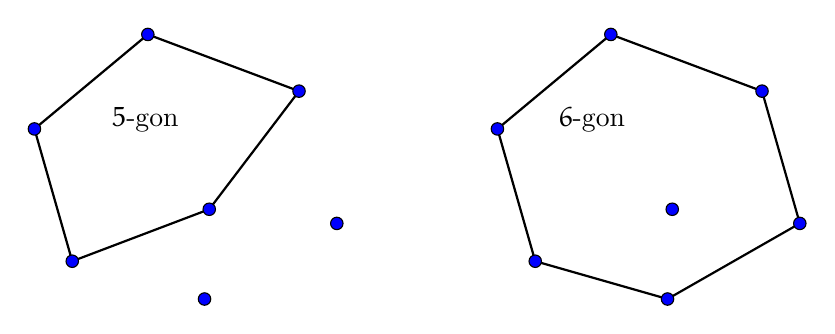
\begin{tikzpicture}[scale=1.5]
\newcommand\x{1.5}
  \draw[thick]
    (-.56, 3.48)
     -- (.40, 4.28)
     -- (1.68, 3.80)
     -- (.92, 2.80)
     -- (-.24, 2.36)
     -- (-.56, 3.48);
\vertex{-.56}{3.48}{\x};
\vertex{.40}{4.28}{\x};
\vertex{1.68}{3.80}{\x};
\vertex{2.00}{2.68}{\x};
\vertex{.88}{2.04}{\x};
\vertex{.92}{2.80}{\x};
\vertex{-.24}{2.36}{\x};
  \draw[thick]
    (3.68, 2.36)
     -- (3.36, 3.48)
     -- (4.32, 4.28)
     -- (5.60, 3.80)
     -- (5.92, 2.68)
     -- (4.80, 2.04)
     -- (3.68, 2.36);
\vertex{3.36}{3.48}{\x};
\vertex{4.32}{4.28}{\x};
\vertex{5.60}{3.80}{\x};
\vertex{5.92}{2.68}{\x};
\vertex{4.80}{2.04}{\x};
\vertex{4.84}{2.80}{\x};
\vertex{3.68}{2.36}{\x};
  \node
     at (.38, 3.56) {$5$-gon};
  \node
     at (4.16, 3.56) {$6$-gon};
\end{tikzpicture}
\end{center}

\begin{theorem}[Erd\H{o}s \& Szekeres 1935]
$\forall k \in \mathbb{N}, \exists$ a smallest integer $g(k)$ such that every set of $g(k)$ points contains a $k$-gon.
\end{theorem}

\pause

\centering

\medskip

\structure{
Is SAT solving suitable to answer such questions? Yes!}

}

\frame{
	\frametitle{Bounds for Small $k$}

\large 

Clearly, it takes exactly three points in general position to have a $3$-gon (triangle)


\bigskip

Some sets of 4 points do not for a $4$-gon:

\bigskip

\centering

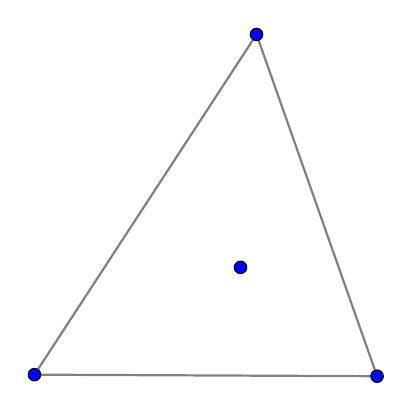
\begin{tikzpicture}[scale=1.5]
\newcommand{\x}{1.5}

  \draw[gray, thick]
    (2.30317, 7.38398)
     -- (3.32398, 4.490406)
     -- (0.42302, 4.503321)
     -- cycle;

\vertex{0.423016}{4.503319}{\x};
\vertex{2.303165}{7.383978}{\x};
\vertex{2.167452}{5.411797}{\x};
\vertex{3.32398}{4.490404}{\x};

\end{tikzpicture}

\bigskip

\pause

\structure{How many points imply a $4$-gon?}

}

\frame{
	\frametitle{Upperbound for $4$-Gon: $g(4) = 5$ \textcolor{xgreen}{[Klein, 1932]}}

\large

   \newcommand{\x}{0.75}


\centering
	
	
\begin{tikzpicture}[scale=2.5]

  \draw[shift={(1, 3.04)}, scale=1.5, thick]
    (0, 0)
     -- (0.64, 0.32)
     -- (1.12, 0)
     -- (0.8, -0.48)
     -- (0.32, -0.48)
     -- cycle;

\only<2->{
  \filldraw[shift={(1, 3.04)}, scale=1.5, draw=structure, very thick, fill=structure!30!white]
    (0, 0)
     -- (0.64, 0.32)
     -- (1.12, 0)
 %    -- (0.8, -0.48)
     -- (0.32, -0.48)
     -- cycle;     
}
     
  \vertex{2.2}{2.32}{\x};
  \vertex{2.68}{3.04}{\x};
  \vertex{1.96}{3.52}{\x};
  \vertex{1}{3.04}{\x};
  \vertex{1.48}{2.32}{\x};

\end{tikzpicture}
~~~~~~~~~~~~~~~~~~~~
\pause
\pause
\begin{tikzpicture}[scale=2.5]
  \draw[shift={(3.8, 2.32)}, scale=1.5, thick]
    (0, 0)
     -- (0, 0.8)
     -- (0.8, 0.64)
     -- (0.64, 0.16)
     -- cycle;

%  \draw[shift={(3.8, 3.52)}, scale=1.5]
%    (0, 0)
%     -- (0.64, -0.64);
%  \draw[shift={(3.8, 2.32)}, scale=1.5]
%    (0, 0)
%     -- (0.8, 0.64);

\only<4->{
  \filldraw[shift={(3.8, 2.32)}, scale=1.5, draw=structure, very thick, fill=structure!30!white]
    (0, 0)
     -- (0, 0.8)
     -- (0.8, 0.64)
     -- (0.64, 0.16)
     -- cycle;
%    (0, 0)
%     -- (0.16, -0.48)
%     -- (0.64, -0.64)
%     -- (0.8, -0.16)
%     -- cycle;
     
%   \draw[shift={(3.8, 3.52)}, scale=1.5]
%    (0, 0)
%     -- (0.64, -0.64);
%  \draw[shift={(3.8, 2.32)}, scale=1.5]
%    (0, 0)
%     -- (0.8, 0.64);
}

  \vertex{4.04}{2.8}{\x};
  \vertex{3.8}{3.52}{\x};
  \vertex{5}{3.28}{\x};
  \vertex{4.76}{2.56}{\x};
  \vertex{3.8}{2.32}{\x};

\end{tikzpicture}

\vspace{-20pt}

\pause
\pause
	
\begin{tikzpicture}[scale=2.5]
     
  
    \draw[shift={(5.72, 2.56)}, scale=1.5]
    (0, 0)
     -- (1.28, 0.48);

  \draw[shift={(5.96, 2.32)}, scale=1.5, thick]
    (0, 0)
     -- (0.48, 0.96)
     -- (0.96, 0.16)
     -- cycle;

\only<6->{

    \draw[shift={(5.72, 2.56)}, scale=1.5]
    (0, 0)
     -- (1.28, 0.48);
     
  \filldraw[shift={(5.96, 2.32)}, scale=1.5, draw=structure, very thick, fill=structure!30!white]
    (0, 0)
     -- (0.3426, 0.348475)
     -- (0.59104, 0.44164)
     -- (0.96, 0.16)
     -- cycle;
 }
 
  \vertex{6.4739}{2.842713}{\x};
  \vertex{6.84656}{2.98246}{\x};
  \vertex{5.96}{2.32}{\x};
  \vertex{6.68}{3.76}{\x};
  \vertex{7.4}{2.56}{\x};
  

  \end{tikzpicture}	
  
\pause
\pause
\bigskip

\centering

\structure{Happy ending problem}

}

\frame{
	\frametitle{Bound Results for $5$-Gon and $6$-Gon}


\large

\begin{minipage}{0.45\textwidth}
$g(5) = 9$
\begin{itemize}
\item \textcolor{xgreen}{[Kalbfleisch \& Stanton '70]\!\!\!\!\!\!\!\!\!\!}
\end{itemize}
\end{minipage}
\begin{minipage}{0.45\textwidth}
\centering
\medskip
~~~~~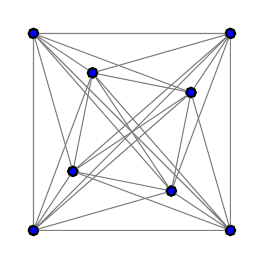
\begin{tikzpicture}[scale=0.5]

\node[draw,circle, thick, fill=blue, scale=0.3] (a) at (0,0) {};
\node[draw,circle, thick, fill=blue, scale=0.3] (b) at (5,0) {};
\node[draw,circle, thick, fill=blue, scale=0.3] (c) at (0,5) {};
\node[draw,circle, thick, fill=blue, scale=0.3] (d) at (5,5) {};

\node[draw,circle, thick, fill=blue, scale=0.3] (e) at (1,1.5) {};
\node[draw,circle, thick, fill=blue, scale=0.3] (f) at (3.5,1) {};
\node[draw,circle, thick, fill=blue, scale=0.3] (g) at (1.5,4) {};
\node[draw,circle, thick, fill=blue, scale=0.3] (h) at (4,3.5) {};

\draw[gray] (a) -- (b) (a) -- (c) (a) -- (d) (a) -- (e) (a) -- (f) (a) -- (g) (a) -- (h);
\draw[gray] (b) -- (c) (b) -- (d) (b) -- (e) (b) -- (f) (b) -- (g) (b) -- (h);
\draw[gray] (c) -- (d) (c) -- (e) (c) -- (f) (c) -- (g) (c) -- (h);
\draw[gray] (d) -- (e) (d) -- (f) (d) -- (g) (d) -- (h);
\draw[gray] (e) -- (f) (e) -- (g) (e) -- (h);
\draw[gray] (f) -- (g) (f) -- (h)  (g) -- (h);
 
\end{tikzpicture}
\end{minipage}


\begin{minipage}{0.45\textwidth}
\centering
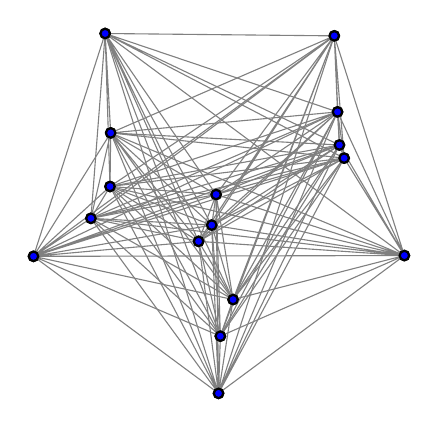
\begin{tikzpicture}[scale=1]

\node[draw,circle, thick, fill=blue, scale=0.3] (a) at (0.19, 1.95) {};
\node[draw,circle, thick, fill=blue, scale=0.3] (b) at (2.54, 0.21) {};
\node[draw,circle, thick, fill=blue, scale=0.3] (c) at (4.9, 1.96) {};
\node[draw,circle, thick, fill=blue, scale=0.3] (d) at (4.01, 4.75) {};
\node[draw,circle, thick, fill=blue, scale=0.3] (e) at (1.1, 4.78) {};
\node[draw,circle, thick, fill=blue, scale=0.3] (f) at (2.5091, 2.735) {};
\node[draw,circle, thick, fill=blue, scale=0.3] (g) at (1.1702, 3.5174) {};
\node[draw,circle, thick, fill=blue, scale=0.3] (h) at (4.0512, 3.7842) {};
\node[draw,circle, thick, fill=blue, scale=0.3] (i) at (2.7243, 1.4014) {};
\node[draw,circle, thick, fill=blue, scale=0.3] (j) at (0.9192, 2.4327) {};
\node[draw,circle, thick, fill=blue, scale=0.3] (k) at (4.1349, 3.1973) {};
\node[draw,circle, thick, fill=blue, scale=0.3] (l) at (2.2864, 2.1402) {};
\node[draw,circle, thick, fill=blue, scale=0.3] (m) at (2.5628, 0.9363) {};
\node[draw,circle, thick, fill=blue, scale=0.3] (n) at (1.1617, 2.8371) {};
\node[draw,circle, thick, fill=blue, scale=0.3] (o) at (2.4537, 2.3468) {};
\node[draw,circle, thick, fill=blue, scale=0.3] (p) at (4.0752, 3.364) {};
 
 
\draw[gray] (a) -- (b) (a) -- (c) (a) -- (d) (a) -- (e) (a) -- (f) (a) -- (g) (a) -- (h) (a) -- (i) (a) -- (j) (a) -- (k) (a) -- (l) (a) -- (m) (a) -- (n) (a) -- (o) (a) -- (p);
\draw[gray] (b) -- (c) (b) -- (d) (b) -- (e) (b) -- (f) (b) -- (g) (b) -- (h) (b) -- (i) (b) -- (j) (b) -- (k) (b) -- (l) (b) -- (m) (b) -- (n) (b) -- (o) (b) -- (p);
\draw[gray] (c) -- (d) (c) -- (e) (c) -- (f) (c) -- (g) (c) -- (h) (c) -- (i) (c) -- (j) (c) -- (k) (c) -- (l) (c) -- (m) (c) -- (n) (c) -- (o) (c) -- (p);
\draw[gray] (d) -- (e) (d) -- (f) (d) -- (g) (d) -- (h) (d) -- (i) (d) -- (j) (d) -- (k) (d) -- (l) (d) -- (m) (d) -- (n) (d) -- (o) (d) -- (p);
\draw[gray] (e) -- (f) (e) -- (g) (e) -- (h) (e) -- (i) (e) -- (j) (e) -- (k) (e) -- (l) (e) -- (m) (e) -- (n) (e) -- (o) (e) -- (p);
\draw[gray] (f) -- (g) (f) -- (h) (f) -- (i) (f) -- (j) (f) -- (k) (f) -- (l) (f) -- (m) (f) -- (n) (f) -- (o) (f) -- (p);
\draw[gray] (g) -- (h) (g) -- (i) (g) -- (j) (g) -- (k) (g) -- (l) (g) -- (m) (g) -- (n) (g) -- (o) (g) -- (p);
\draw[gray] (h) -- (i) (h) -- (j) (h) -- (k) (h) -- (l) (h) -- (m) (h) -- (n) (h) -- (o) (h) -- (p);
\draw[gray] (i) -- (j) (i) -- (k) (i) -- (l) (i) -- (m) (i) -- (n) (i) -- (o) (i) -- (p);
\draw[gray] (j) -- (k) (j) -- (l) (j) -- (m) (j) -- (n) (j) -- (o) (j) -- (p);
\draw[gray] (k) -- (l) (k) -- (m) (k) -- (n) (k) -- (o) (k) -- (p);
\draw[gray] (l) -- (m) (l) -- (n) (l) -- (o) (l) -- (p);
\draw[gray] (m) -- (n) (m) -- (o) (m) -- (p);
\draw[gray] (n) -- (o) (n) -- (p) (o) -- (p); 
 
 \node[draw,circle, thick, fill=blue, scale=0.3] (a) at (0.19, 1.95) {};
\node[draw,circle, thick, fill=blue, scale=0.3] (b) at (2.54, 0.21) {};
\node[draw,circle, thick, fill=blue, scale=0.3] (c) at (4.9, 1.96) {};
\node[draw,circle, thick, fill=blue, scale=0.3] (d) at (4.01, 4.75) {};
\node[draw,circle, thick, fill=blue, scale=0.3] (e) at (1.1, 4.78) {};
\node[draw,circle, thick, fill=blue, scale=0.3] (f) at (2.5091, 2.735) {};
\node[draw,circle, thick, fill=blue, scale=0.3] (g) at (1.1702, 3.5174) {};
\node[draw,circle, thick, fill=blue, scale=0.3] (h) at (4.0512, 3.7842) {};
\node[draw,circle, thick, fill=blue, scale=0.3] (i) at (2.7243, 1.4014) {};
\node[draw,circle, thick, fill=blue, scale=0.3] (j) at (0.9192, 2.4327) {};
\node[draw,circle, thick, fill=blue, scale=0.3] (k) at (4.1349, 3.1973) {};
\node[draw,circle, thick, fill=blue, scale=0.3] (l) at (2.2864, 2.1402) {};
\node[draw,circle, thick, fill=blue, scale=0.3] (m) at (2.5628, 0.9363) {};
\node[draw,circle, thick, fill=blue, scale=0.3] (n) at (1.1617, 2.8371) {};
\node[draw,circle, thick, fill=blue, scale=0.3] (o) at (2.4537, 2.3468) {};
\node[draw,circle, thick, fill=blue, scale=0.3] (p) at (4.0752, 3.364) {};
 
\end{tikzpicture}
\end{minipage}
~~~
\begin{minipage}{0.45\textwidth}
\medskip
$g(6) = 17$
\begin{itemize}
\item Computer-assisted proof, 1500 CPU hours \textcolor{xgreen}{[SzekeresPeters '06]}
\item One CPU hour using a SAT solver \textcolor{xgreen}{[Scheucher '18]\!\!\!\!\!\!\!\!\!\!}
\item Only $10$ seconds using new encoding\!\!\!\!\!\!\!\!\!\!\!\!
\end{itemize}
\end{minipage}

}


\frame{
	\frametitle{Bound History}

\large

\begin{theorem}[\textcolor{xgreen}{Erd\H{o}s \& Szekeres '35, '60}]
$2^{k-2} +1 \leq g(k) \leq \binom{2k-4}{k-2}+1$~~~~~($\mathrm{of~magnitude}$ $4^{k-o(k)}$)
\end{theorem}

\begin{itemize}
\item Equality with lower bound conjectured by Szekeres
\item Erd\H{o}s offered \$500 for a proof
\end{itemize}

\bigskip

\begin{theorem}[\textcolor{xgreen}{Suk ’16}]
$g(k) \leq 2^{k+o(k)}$ 
\end{theorem}

\bigskip

\begin{theorem}[\textcolor{xgreen}{Holmsen, Mojarrad, Pach, and Tardos ’17}]
$g(k) \leq 2^{k+O(\sqrt{k log k})}$
\end{theorem}	

}

\frame{
	\frametitle{$k$-Holes}
	
\large

A \structure{$k$-hole} (in $S$) is a $k$-gon
containing no other points of $S$. 

\medskip

\begin{center}
\begin{tikzpicture}[scale=1.5]
\newcommand\x{1}
  \filldraw[thick, draw=xgreen, fill=xgreen!30!white]
    (-.56, 3.48)
     -- (.40, 4.28)
     -- (1.68, 3.80)
     -- (.92, 2.80)
     -- (-.24, 2.36)
     -- (-.56, 3.48);
\vertex{-.56}{3.48}{\x};
\vertex{.40}{4.28}{\x};
\vertex{1.68}{3.80}{\x};
\vertex{2.00}{2.68}{\x};
\vertex{.88}{2.04}{\x};
\vertex{.92}{2.80}{\x};
\vertex{-.24}{2.36}{\x};
  \filldraw[thick, draw=structure, fill=structure!30!white]
    (3.68, 2.36)
     -- (3.36, 3.48)
     -- (4.32, 4.28)
     -- (5.60, 3.80)
     -- (5.92, 2.68)
     -- (4.80, 2.04)
     -- (3.68, 2.36);
\vertex{3.36}{3.48}{\x};
\vertex{4.32}{4.28}{\x};
\vertex{5.60}{3.80}{\x};
\vertex{5.92}{2.68}{\x};
\vertex{4.80}{2.04}{\x};
\vertex{4.84}{2.80}{\x};
\vertex{3.68}{2.36}{\x};
  \node
     at (.38, 3.56) {$5$-hole};
  \node
     at (4.46, 3.56) {not a $6$-hole};
\end{tikzpicture}
\end{center}

\pause

Let \structure{$h(k)$} denote the \structure{smallest} number of points that contain a $k$-hole.

\bigskip

Erd\H{o}s, 1970’s: For $k$ fixed, does every \structure{sufficiently large}
point set contain $k$-holes?

}

\frame{
	\frametitle{$k$-Holes Overview}

\large

A \structure{$k$-hole} (in $S$) is a $k$-gon
containing no other points of $S$. 

\bigskip

Erd\H{o}s, 1970’s: For $k$ fixed, does every \structure{sufficiently large}
point set contain $k$-holes?
\begin{itemize}
\item $3$ points $\Rightarrow \exists$ $3$-hole
\item $5$ points $\Rightarrow \exists$ $4$-hole
\item $10$ points $\Rightarrow \exists$ $5$-hole \textcolor{xgreen}{[Harborth ’78]}
\item Arbitrarily large point sets with no $7$-hole  \textcolor{xgreen}{[Horton ’83]}
\end{itemize}

\bigskip

Main open question: what about $6$-hole?
\begin{itemize}
\item Sufficiently large point sets contain a $6$-hole\\
\textcolor{xgreen}{[Gerken ’08 and Nicol\'as ’07, independently]}
\item \structure{Conjecture}: $h(6) = 30$
\end{itemize}

}

\section{$k$-Hole Results}
\frame{\Large \tableofcontents[currentsection]}

\frame{
	\frametitle{Lowerbound for $4$-Hole: $h(4) > 4$}
	
	\large
	
	Same example as $g(4) > 4$:
	
	\bigskip
	\centering
	
	
	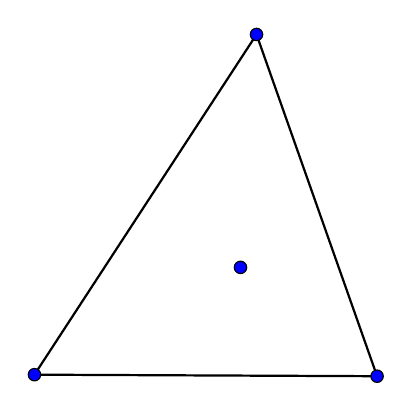
\begin{tikzpicture}[scale=1.5]
\newcommand{\x}{1.5}


  \draw[ thick]
    (2.30317, 7.38398)
     -- (3.32398, 4.490406)
     -- (0.42302, 4.503321)
     -- cycle;

\vertex{0.423016}{4.503319}{\x};
\vertex{2.303165}{7.383978}{\x};
\vertex{2.167452}{5.411797}{\x};
\vertex{3.32398}{4.490404}{\x};

\end{tikzpicture}
	
}

\frame{
	\frametitle{Upperbound for $4$-Hole: $h(4) = 5$}

\large

Recall that every set of 5 points contains a $4$-gon

\bigskip

Every $4$-gon is either a $4$-hole or contains a $4$-hole

\bigskip
\bigskip

   \newcommand{\x}{0.75}


\centering
	
	
%\begin{tikzpicture}[scale=2.5]
%
%  \draw[shift={(1, 3.04)}, scale=1.5, thick]
%    (0, 0)
%     -- (0.64, 0.32)
%     -- (1.12, 0)
%     -- (0.8, -0.48)
%     -- (0.32, -0.48)
%     -- cycle;
%
%\only<2->{
%  \filldraw[shift={(1, 3.04)}, scale=1.5, draw=structure, very thick, fill=structure!30!white]
%    (0, 0)
%     -- (0.64, 0.32)
%     -- (1.12, 0)
% %    -- (0.8, -0.48)
%     -- (0.32, -0.48)
%     -- cycle;     
%}
%     
%  \vertex{2.2}{2.32}{\x};
%  \vertex{2.68}{3.04}{\x};
%  \vertex{1.96}{3.52}{\x};
%  \vertex{1}{3.04}{\x};
%  \vertex{1.48}{2.32}{\x};
%
%\end{tikzpicture}
%~~~~~~~~~~~~~~~~~~~~
%\pause
%\pause
\begin{tikzpicture}[scale=2.5]
  \draw[shift={(3.8, 2.32)}, scale=1.5, thick]
    (0, 0)
     -- (0, 0.8)
     -- (0.8, 0.64)
     -- (0.64, 0.16)
     -- cycle;

  \draw[shift={(3.8, 3.52)}, scale=1.5]
    (0, 0)
     -- (0.64, -0.64);
  \draw[shift={(3.8, 2.32)}, scale=1.5]
    (0, 0)
     -- (0.8, 0.64);

\only<2->{
  \filldraw[shift={(3.8, 3.52)}, scale=1.5, draw=structure, very thick, fill=structure!30!white]
    (0, 0)
     -- (0.16, -0.48)
     -- (0.64, -0.64)
     -- (0.8, -0.16)
     -- cycle;
     
   \draw[shift={(3.8, 3.52)}, scale=1.5]
    (0, 0)
     -- (0.64, -0.64);
  \draw[shift={(3.8, 2.32)}, scale=1.5]
    (0, 0)
     -- (0.8, 0.64);
}

  \vertex{4.04}{2.8}{\x};
  \vertex{3.8}{3.52}{\x};
  \vertex{5}{3.28}{\x};
  \vertex{4.76}{2.56}{\x};
  \vertex{3.8}{2.32}{\x};

\end{tikzpicture}

%\pause
%\pause
%	
%\begin{tikzpicture}[scale=2.5]
%     
%  
%    \draw[shift={(5.72, 2.56)}, scale=1.5]
%    (0, 0)
%     -- (1.28, 0.48);
%
%  \draw[shift={(5.96, 2.32)}, scale=1.5, thick]
%    (0, 0)
%     -- (0.48, 0.96)
%     -- (0.96, 0.16)
%     -- cycle;
%
%\only<6->{
%
%    \draw[shift={(5.72, 2.56)}, scale=1.5]
%    (0, 0)
%     -- (1.28, 0.48);
%     
%  \filldraw[shift={(5.96, 2.32)}, scale=1.5, draw=structure, very thick, fill=structure!30!white]
%    (0, 0)
%     -- (0.3426, 0.348475)
%     -- (0.59104, 0.44164)
%     -- (0.96, 0.16)
%     -- cycle;
% }
% 
%  \vertex{6.4739}{2.842713}{\x};
%  \vertex{6.84656}{2.98246}{\x};
%  \vertex{5.96}{2.32}{\x};
%  \vertex{6.68}{3.76}{\x};
%  \vertex{7.4}{2.56}{\x};
%  
%
%  \end{tikzpicture}
	
}

\frame{
	\frametitle{Lowerbound for $5$-Hole: $h(5) \geq 10$}

\large

\begin{center}
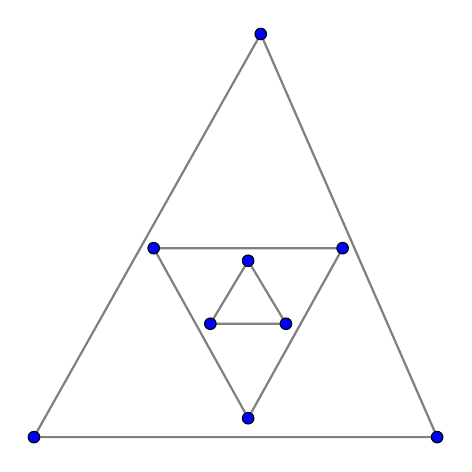
\begin{tikzpicture}[scale=1.6]
\newcommand{\x}{1.3}


%\draw[gray, thick]
%  (3.69386, 5.06637)
%   -- (4.98988, 1.34029)
%   -- (1.26017, 1.37339)
%   -- cycle;
%\draw[gray, thick]
%  (2.22254, 2.50733)
%   -- (4.10115, 3.38951)
%   -- (3.09768, 1.62184)
%   -- cycle;
%\draw[gray, thick]
%  (2.22254, 2.50733)
%   -- (4.10115, 3.38951)
%   -- (3.09768, 1.62184)
%   -- cycle;
%\draw[gray, thick]
%  (2.97385, 2.38629)
%   -- (3.4507, 3.01154)
%   -- (3.50817, 2.53151)
%   -- cycle;
   
%\vertex{1.26017}{1.37339}{\x};
%\vertex{3.69386}{5.06637}{\x};
%\vertex{4.10115}{3.38951}{\x};
%\vertex{2.22253}{2.50734}{\x};
%\vertex{3.4507}{3.01154}{\x};
%\vertex{2.97385}{2.38629}{\x};
%\vertex{3.50817}{2.53151}{\x};
%\vertex{3.09768}{1.62184}{\x};
%\vertex{4.98988}{1.34029}{\x};

\draw[gray, thick]
  (-0.3, 0)
   -- (0.3, 0)
   -- (0, 0.5)
   -- cycle;
   
\draw[gray, thick]
  (-0.75, 0.6)
   -- (0.75, 0.6)
   -- (0, -0.75)
   -- cycle;

\draw[gray, thick]
  (-1.7, -0.9)
   -- (1.5, -0.9)
   -- (0.1, 2.3)
   -- cycle;

\vertex{-0.3}{0}{\x};
\vertex{0.3}{0}{\x};
\vertex{0}{0.5}{\x};

\vertex{0.75}{0.6}{\x};
\vertex{-0.75}{0.6}{\x};
\vertex{0}{-0.75}{\x};

\vertex{1.5}{-0.9}{\x};
\vertex{-1.7}{-0.9}{\x};
\vertex{0.1}{2.3}{\x};

%  \filldraw[shift={(0, 0)}, scale=1.5, draw=structure, very thick, fill=structure!30!white]
%    (1.26017, 1.37339)
%     -- (3.69386, {5.06637)
%     -- (4.10115, 3.38951)
%     -- (2.22253, 2.50734)
%     -- cycle;
 

\end{tikzpicture}
\end{center}

All $5$-gons in these 9 points have an inner point: $h(5) = 10$
	
}

\frame{
	\frametitle{Lowerbound for $6$-Hole: $h(6) \geq 30$}

\large

\vspace{-10pt}

\begin{center}
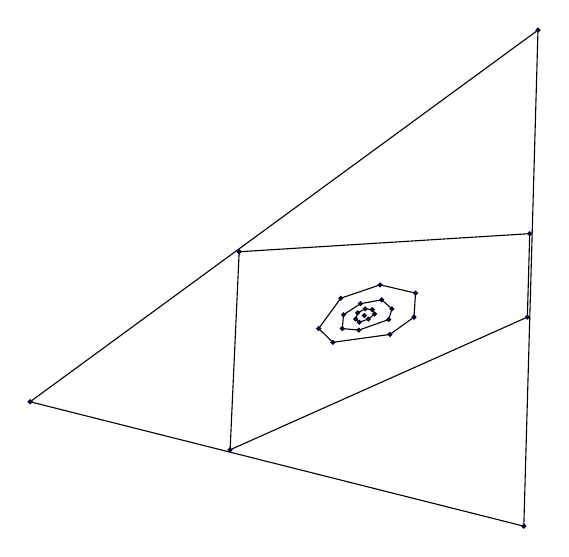
\begin{tikzpicture}[scale=0.5]

%  \node at (8,12.5) {
%  coordinates:};
%  
%  \node at (8,10) {
%\begin{tabular}{r@{~~\,}r}
%1 &1260 \\
%16  &743\\
%22 & 531\\
%37 & 0\\
%306 & 592\\
%310 & 531\\
%366 & 552\\
%371 & 487\\
%374 & 525\\
%~& ~\\
%  \end{tabular}
%  };
%
%\node at (10,10) {
%\begin{tabular}{r@{~~\,}r}
%392 & 575 \\
%396 & 613 \\
%410 & 539 \\
%416 & 550 \\
%426 & 526 \\
%434 & 552 \\
%436 & 535 \\
%446 & 565 \\
%449 & 518 \\
%450 & 498 \\
%  \end{tabular}
%  };  
%  
%\node at (12,10) {
%\begin{tabular}{r@{~~\,}r}
%453 & 542 \\
%458 & 526 \\
%489 & 537 \\
%492 & 502 \\
%496 & 579 \\
%516 & 467 \\
%552 & 502 \\
%754 & 697 \\
%777 & 194 \\
%1259 & 320 \\
%  \end{tabular}
%  };  
  
  \tikzset{vertex/.style={draw, circle, fill=blue, scale=0.12}}
     
\node[vertex] (aa) at (0.05,12.60) {};
\node[vertex] (ab) at (-.31,0) {};
\node[vertex] (ac) at (-12.85,3.16) {};

\node[vertex] (bb) at (-.16,7.43) {};
\node[vertex] (ba) at (-.22,5.31) {};
\node[vertex] (c) at (-3.06,5.92) {};
\node[vertex] (d) at (-3.10,5.31) {};
\node[vertex] (e) at (-3.66,5.52) {};
\node[vertex] (f) at (-3.71,4.87) {};
\node[vertex] (g) at (-3.74,5.25) {};
\node[vertex] (h) at (-3.92,5.75) {};
\node[vertex] (i) at (-3.96,6.13) {};
\node[vertex] (j) at (-4.10,5.39) {};
\node[vertex] (k) at (-4.16,5.50) {};
\node[vertex] (l) at (-4.26,5.26) {};
\node[vertex] (m) at (-4.34,5.52) {};
\node[vertex] (n) at (-4.36,5.35) {};
\node[vertex] (o) at (-4.46,5.65) {};
\node[vertex] (p) at (-4.49,5.18) {};
\node[vertex] (q) at (-4.50,4.98) {};
\node[vertex] (r) at (-4.53,5.42) {};
\node[vertex] (s) at (-4.58,5.26) {};
\node[vertex] (t) at (-4.89,5.37) {};
\node[vertex] (u) at (-4.92,5.02) {};
\node[vertex] (v) at (-4.96,5.79) {};
\node[vertex] (w) at (-5.16,4.67) {};
\node[vertex] (x) at (-5.52,5.02) {};
\node[vertex] (bc) at (-7.54,6.97) {};
\node[vertex] (bd) at (-7.77,1.94) {};

\draw[] (aa) -- (ab) -- (ac) -- (aa);
\draw[] (ba) -- (bb) -- (bc) -- (bd) -- (ba);

\draw[] (x) -- (v) -- (i) -- (c) -- (d) -- (f) --(w) -- (x)  ;

\draw[] (t) -- (o)-- (h) -- (e) -- (g) --(q) --(u) --(t)  ;

\draw[] (s) -- (r) -- (m)-- (k) -- (j) -- (l) -- (p) -- (s)  ;

\end{tikzpicture}
\end{center}

\vspace{-10pt}

29 points, no $6$-hole \textcolor{xgreen}{[Overmars ’02]}
\begin{itemize}
\item Found using simulated annealing... is now \structure{easy using SAT}
\item This contains $7$-gons. Each $9$-gon contains a $6$-hole
\end{itemize}

}

\frame{
	\frametitle{No Lowerbound for $7$-Hole: Horton's Construction (I)}


\bigskip
\bigskip

\begin{minipage}{.45\textwidth}
\centering

\begin{tikzpicture}[scale=1.5]

\node[draw,circle, fill=blue, scale=0.3] (a) at (2.786402,4.8952) {};
\node[draw,circle, fill=structure, scale=0.3] (b) at (0.6552,4.8952) {};


\draw[gray] (a) -- (b) ;


 
\end{tikzpicture}

\bigskip

$2^1$ points, no 7-hole

\bigskip
\bigskip
\bigskip

\pause

\begin{tikzpicture}[scale=1.5]

\node[draw,circle, fill=structure, scale=0.3] (a) at (2.786402,4.8952) {};
\node[draw,circle, fill=blue, scale=0.3] (c) at (3.852003,5.8276) {};
\node[draw,circle, fill=structure, scale=0.3] (b) at (0.6552,4.8952) {};
\node[draw,circle, fill=blue, scale=0.3] (d) at (1.720801,5.8276) {};


\draw[structure, thick] (a) -- (b) ;
\draw[gray] (a) -- (c) (a) -- (d) (b) -- (c) (b) -- (d) ; 
\draw[blue, thick] (c) -- (d); 

 
\end{tikzpicture}

\bigskip

$2^2$ points, no 7-hole

\end{minipage}
~~~\pause
\begin{minipage}{.45\textwidth}
\centering
\begin{tikzpicture}[scale=1.5]

\node[draw,circle, fill=structure, scale=0.3] (a) at (2.786402,4.8952) {};
\node[draw,circle, fill=structure, scale=0.3] (b) at (3.852003,5.8276) {};
\node[draw,circle, fill=structure, scale=0.3] (c) at (0.6552,4.8952) {};
\node[draw,circle, fill=structure, scale=0.3] (d) at (1.720801,5.8276) {};

\node[draw,circle, fill=blue, scale=0.3] (e) at (1.188,7.6924) {};
\node[draw,circle, fill=blue, scale=0.3] (f) at (3.319199,7.6924) {};
\node[draw,circle, fill=blue, scale=0.3] (g) at (2.253598,8.6248) {};
\node[draw,circle, fill=blue, scale=0.3] (h) at (4.3848,8.6248) {};

\draw[structure, thick] (a) -- (b) (a) -- (c) (a) -- (d) (c) -- (d) (b) -- (c) (b) -- (d);
\draw[gray]  (a) -- (e) (a) -- (f) (a) -- (g) (a) -- (h) (b) -- (e) (b) -- (f) (b) -- (g) (b) -- (h);
\draw[gray] (c) -- (d)  (c) -- (e) (c) -- (f) (c) -- (g) (c) -- (h);
\draw[gray] (d) -- (e) (d) -- (f) (d) -- (g) (d) -- (h);
\draw[blue, thick] (e) -- (f) (e) -- (g) (e) -- (h);
\draw[blue, thick] (f) -- (g) (f) -- (h)  (g) -- (h);


 
\end{tikzpicture}

\bigskip

$2^3$ points, no 7-hole
\end{minipage}
	
}

\iffalse
\frame{
	\frametitle{No Lowerbound for $7$-Hole: Horton's Construction (II)}

\centering

\begin{tikzpicture}[scale=1.7]

\node[draw,circle, fill=structure, scale=0.3] (a) at (0.6552, 5.1752) {};
\node[draw,circle, fill=structure, scale=0.3] (b) at (2.644318, 5.1752) {};
\node[draw,circle, fill=structure, scale=0.3] (c) at (1.649762, 5.29175) {};
\node[draw,circle, fill=structure, scale=0.3] (d) at (3.63888, 5.29175) {};
\node[draw,circle, fill=structure, scale=0.3] (e) at (1.15248, 5.52485) {};
\node[draw,circle, fill=structure, scale=0.3] (f) at (3.141602, 5.52485) {};
\node[draw,circle, fill=structure, scale=0.3] (g) at (2.14704, 5.6414) {};
\node[draw,circle, fill=structure, scale=0.3] (h) at (4.136158, 5.6414) {};
\node[draw,circle, fill=blue, scale=0.3] (i) at (0.90384, 8.4386) {};
\node[draw,circle, fill=blue, scale=0.3] (j) at (2.89296, 8.4386) {};
\node[draw,circle, fill=blue, scale=0.3] (k) at (1.898398, 8.55515) {};
\node[draw,circle, fill=blue, scale=0.3] (l) at (3.887522, 8.55515) {};
\node[draw,circle, fill=blue, scale=0.3] (m) at (1.40112, 8.78825) {};
\node[draw,circle, fill=blue, scale=0.3] (n) at (3.390238, 8.78825) {};
\node[draw,circle, fill=blue, scale=0.3] (o) at (2.395682, 8.9048) {};
\node[draw,circle, fill=blue, scale=0.3] (p) at (4.3848, 8.9048) {};
 
 
\draw[structure,thick] (a) -- (b) (a) -- (c) (a) -- (d) (a) -- (e) (a) -- (f) (a) -- (g) (a) -- (h);
\draw[structure,thick] (b) -- (c) (b) -- (d) (b) -- (e) (b) -- (f) (b) -- (g) (b) -- (h);
\draw[structure,thick] (c) -- (d) (c) -- (e) (c) -- (f) (c) -- (g) (c) -- (h);
\draw[structure,thick] (d) -- (e) (d) -- (f) (d) -- (g) (d) -- (h); 
\draw[structure,thick] (e) -- (f) (e) -- (g) (e) -- (h) ;
\draw[structure,thick] (f) -- (g) (f) -- (h) ;
\draw[structure,thick] (g) -- (h) ;
\draw[gray] (a) -- (i) (a) -- (j) (a) -- (k) (a) -- (l) (a) -- (m) (a) -- (n) (a) -- (o) (a) -- (p);
\draw[gray] (b) -- (i) (b) -- (j) (b) -- (k) (b) -- (l) (b) -- (m) (b) -- (n) (b) -- (o) (b) -- (p);
\draw[gray] (c) -- (i) (c) -- (j) (c) -- (k) (c) -- (l) (c) -- (m) (c) -- (n) (c) -- (o) (c) -- (p);
\draw[gray] (d) -- (i) (d) -- (j) (d) -- (k) (d) -- (l) (d) -- (m) (d) -- (n) (d) -- (o) (d) -- (p);
\draw[gray] (e) -- (i) (e) -- (j) (e) -- (k) (e) -- (l) (e) -- (m) (e) -- (n) (e) -- (o) (e) -- (p);
\draw[gray] (f) -- (i) (f) -- (j) (f) -- (k) (f) -- (l) (f) -- (m) (f) -- (n) (f) -- (o) (f) -- (p);
\draw[gray] (g) -- (i) (g) -- (j) (g) -- (k) (g) -- (l) (g) -- (m) (g) -- (n) (g) -- (o) (g) -- (p);
 \draw[gray] (h) -- (i) (h) -- (j) (h) -- (k) (h) -- (l) (h) -- (m) (h) -- (n) (h) -- (o) (h) -- (p);
\draw[blue,thick] (i) -- (j) (i) -- (k) (i) -- (l) (i) -- (m) (i) -- (n) (i) -- (o) (i) -- (p);
\draw[blue,thick] (j) -- (k) (j) -- (l) (j) -- (m) (j) -- (n) (j) -- (o) (j) -- (p);
\draw[blue,thick] (k) -- (l) (k) -- (m) (k) -- (n) (k) -- (o) (k) -- (p);
\draw[blue,thick] (l) -- (m) (l) -- (n) (l) -- (o) (l) -- (p);
\draw[blue,thick] (m) -- (n) (m) -- (o) (m) -- (p);
\draw[blue,thick] (n) -- (o) (n) -- (p) (o) -- (p);
 
 \node[draw,circle, fill=structure, scale=0.3] (a) at (0.6552, 5.1752) {};
\node[draw,circle, fill=structure, scale=0.3] (b) at (2.644318, 5.1752) {};
\node[draw,circle, fill=structure, scale=0.3] (c) at (1.649762, 5.29175) {};
\node[draw,circle, fill=structure, scale=0.3] (d) at (3.63888, 5.29175) {};
\node[draw,circle, fill=structure, scale=0.3] (e) at (1.15248, 5.52485) {};
\node[draw,circle, fill=structure, scale=0.3] (f) at (3.141602, 5.52485) {};
\node[draw,circle, fill=structure, scale=0.3] (g) at (2.14704, 5.6414) {};
\node[draw,circle, fill=structure, scale=0.3] (h) at (4.136158, 5.6414) {};
\node[draw,circle, fill=blue, scale=0.3] (i) at (0.90384, 8.4386) {};
\node[draw,circle, fill=blue, scale=0.3] (j) at (2.89296, 8.4386) {};
\node[draw,circle, fill=blue, scale=0.3] (k) at (1.898398, 8.55515) {};
\node[draw,circle, fill=blue, scale=0.3] (l) at (3.887522, 8.55515) {};
\node[draw,circle, fill=blue, scale=0.3] (m) at (1.40112, 8.78825) {};
\node[draw,circle, fill=blue, scale=0.3] (n) at (3.390238, 8.78825) {};
\node[draw,circle, fill=blue, scale=0.3] (o) at (2.395682, 8.9048) {};
\node[draw,circle, fill=blue, scale=0.3] (p) at (4.3848, 8.9048) {};
 
  
\end{tikzpicture}

\bigskip

 $2^4$ points, no 7-hole


}
\fi

\frame{
	\frametitle{No Lowerbound for $7$-Hole: Horton's Construction (III)}
	
	\centering
	
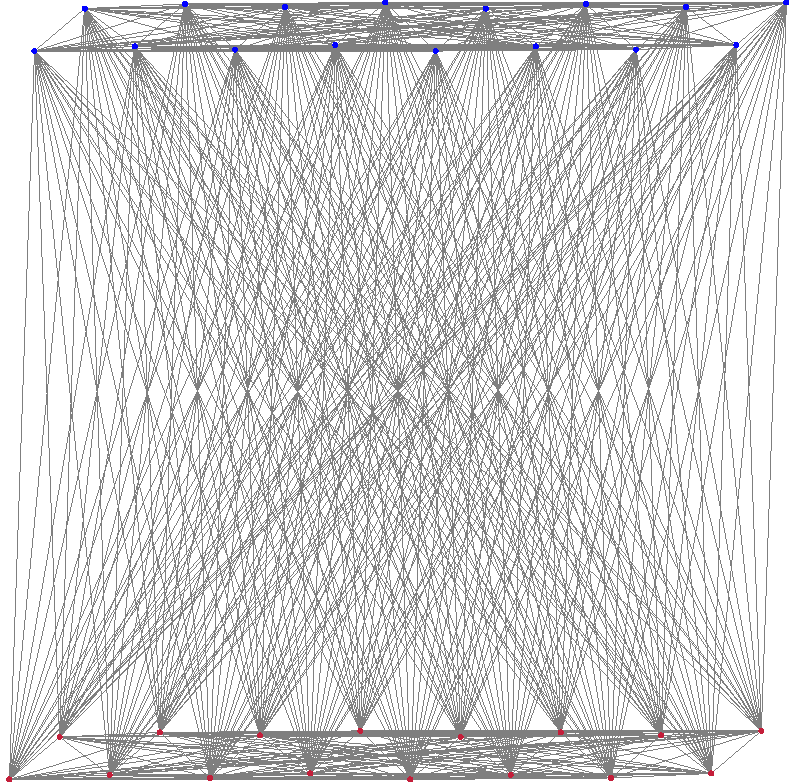
\includegraphics[height=180pt]{7hole-final.pdf}
	
	\bigskip
	
	 $2^5$ points, no 7-hole

}


\section{SAT Encoding}
\frame{\Large \tableofcontents[currentsection]}


\frame{
	\frametitle{Orientation Variables}
	
\large 
\begin{minipage}{.62\textwidth}

\bigskip

No explicit \structure{coordinates} of points

\bigskip

Instead for every triple $a < b < c$,\\ one \structure{orientation variable  $O_{a,b,c}$}
to denote whether point $c$ is above the line $ab$

\bigskip

Triple orientations are enough\\ 
to express $k$-gons and $k$-holes

\bigskip

\only<2->{
WLOG points are \structure{sorted} from left to right\!\!\!\!\!\!\!\!

\bigskip

Not all assignments are \structure{realizable}
\begin{itemize}
\item Realizability is  hard 
\textcolor{xgreen}{[Mnëv '88]}
\item Additional clauses eliminate\\
many unrealizable assignments
\end{itemize}}


\bigskip

\end{minipage}	
\begin{minipage}{.35\textwidth}
\centering
\begin{tikzpicture}
\newcommand{\x}{2}
\node (a) at (2.72, 6.48) {~};
\node (b) at (4.48, 6.24) {~};
\node (c) at (4.72, 7.12) {~};
\node (d) at (4.8, 3.36) {~};

  \draw[shift={(2.24083, 6.54534)}, scale=2]
    (0, 0)
     -- (1.76, -0.24);
  \draw[xgreen, thick, ->]
    (3.2, 6.55)
     .. controls (4.25, 6.35) and (4.4, 6.5) .. (4.5, 6.85);
  \draw[structure, thick, ->]
    (3, 6.2)
     .. controls (4.25, 5.9) and (4.4, 5.8) .. (4.5, 4.4);

%  \draw[shift={(2.8754, 6.36479)}, scale=1, red, very thick, ->]
%    (0, 0)
%     .. controls (1.584, -0.216) and (1.52, -0.4) .. (0.48, -0.72);
  \node[font=\large, text=xgreen]
     at (3.9, 6.65) {+};
  \node[font=\large, text=structure]
     at (3.75, 5.5) {--};
  \node 
     at (2.45, 6.7) {$a$};
  \node
     at (4.74, 6.42) {$b$};
  \node[text=xgreen]
     at (4.85, 7.35) {$c$};
  \node[text=structure]
     at (4.88, 3.12) {$d$};
  \draw[gray]
    (b)
     -- (c)
     -- (a);
  \draw[gray]
    (b)
     -- (d)
     -- (a);
     
\vertex{2.72}{6.48}{\x};
\vertexc{4.8}{3.36}{\x}{structure}; 
\vertex{(4.48}{6.24}{\x};
\vertexc{4.72}{7.12}{\x}{xgreen};
%  \node
%     at (5.07475, 6.26071) {$e$};
%\vertex{0.0491475}{0.0618071}{\x};
\end{tikzpicture}
\end{minipage}
	
}


\iffalse
\frame{
	\frametitle{$k$-Gon Encoding: Forbidding a $k$-Gon}

\large

\begin{minipage}{.47\textwidth}
\centering
$O_{a,b,c} \lor O_{b,c,d} \lor O_{c,d,e} \lor O_{d,e,f}$
\end{minipage}
\hfill
\begin{minipage}{.47\textwidth}
\centering
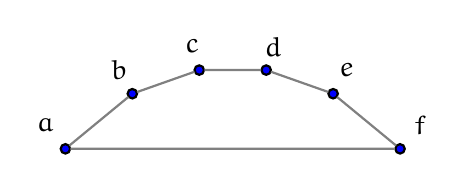
\begin{tikzpicture}[xscale=0.85]
\node at (-0.3,0.3) {$a$};
\node at (0.8,1) {$b$};
\node at (1.9,1.3) {$c$};
\node at (3.1,1.3) {$d$};
\node at (4.2,1) {$e$};
\node at (5.3,0.3) {$f$};
\node[draw,circle, thick, fill=blue, scale=0.3] (a) at (0,0) {};
\node[draw,circle, thick, fill=blue, scale=0.3] (b) at (1,0.7) {};
\node[draw,circle, thick, fill=blue, scale=0.3] (c) at (2,1) {};
\node[draw,circle, thick, fill=blue, scale=0.3] (d) at (3,1) {};
\node[draw,circle, thick, fill=blue, scale=0.3] (e) at (4,0.7) {};
\node[draw,circle, thick, fill=blue, scale=0.3] (f) at (5,0) {};
\draw[gray, thick] (a) -- (b) -- (c) -- (d) -- (e) -- (f) -- (a);
%\draw[gray] (a) -- (b) -- (c) -- (a);
%\draw[gray] (a) -- (c) -- (d) -- (a);
%\draw[gray] (a) -- (d) -- (e) -- (a);
%\draw[gray] (a) -- (e) -- (f) -- (a);
\end{tikzpicture}
\end{minipage}

\begin{minipage}{.47\textwidth}
\centering
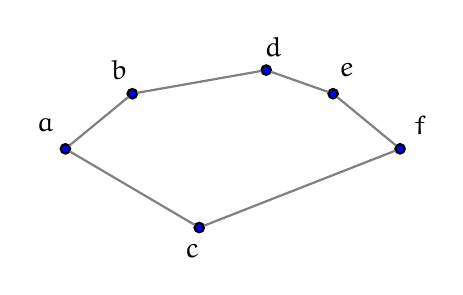
\begin{tikzpicture}[xscale=0.85]
\node at (-0.3,0.3) {$a$};
\node at (0.8,1) {$b$};
\node at (1.9,-1.3) {$c$};
\node at (3.1,1.3) {$d$};
\node at (4.2,1) {$e$};
\node at (5.3,0.3) {$f$};
\node[draw,circle, thick, fill=blue, scale=0.3] (a) at (0,0) {};
\node[draw,circle, thick, fill=blue, scale=0.3] (b) at (1,0.7) {};
\node[draw,circle, thick, fill=blue, scale=0.3] (c) at (2,-1) {};
\node[draw,circle, thick, fill=blue, scale=0.3] (d) at (3,1) {};
\node[draw,circle, thick, fill=blue, scale=0.3] (e) at (4,0.7) {};
\node[draw,circle, thick, fill=blue, scale=0.3] (f) at (5,0) {};
\draw[gray, thick] (a) -- (b) -- (d) -- (e) -- (f) -- (c) -- (a);
%\draw[gray] (a) -- (b) -- (d) -- (a);
%\draw[gray] (a) -- (c) -- (f) -- (a);
%\draw[gray] (a) -- (d) -- (e) -- (a);
%\draw[gray] (a) -- (e) -- (f) -- (a);
\end{tikzpicture}
\end{minipage}
\hfill
\begin{minipage}{.47\textwidth}
$O_{a,b,d} \lor O_{b,d,e} \lor O_{d,e,f} \lor \overline{O_{a,c,f}}$
\end{minipage}


\vspace{-10pt}

\begin{minipage}{.47\textwidth}
$O_{a,b,d} \lor O_{b,d,f} \lor \overline{O_{a,c,e}} \lor \overline{O_{c,e,f}}$
\end{minipage}
\hfill
\begin{minipage}{.47\textwidth}
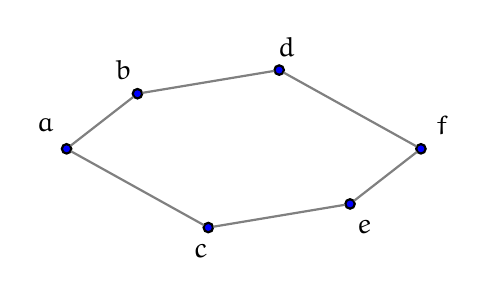
\begin{tikzpicture}[xscale=0.9]
\node at (-0.3,0.3) {$a$};
\node at (0.8,1) {$b$};
\node at (1.9,-1.3) {$c$};
\node at (3.1,1.3) {$d$};
\node at (4.2,-1) {$e$};
\node at (5.3,0.3) {$f$};
\node[draw,circle, thick, fill=blue, scale=0.3] (a) at (0,0) {};
\node[draw,circle, thick, fill=blue, scale=0.3] (b) at (1,0.7) {};
\node[draw,circle, thick, fill=blue, scale=0.3] (c) at (2,-1) {};
\node[draw,circle, thick, fill=blue, scale=0.3] (d) at (3,1) {};
\node[draw,circle, thick, fill=blue, scale=0.3] (e) at (4,-0.7) {};
\node[draw,circle, thick, fill=blue, scale=0.3] (f) at (5,0) {};
\draw[gray, thick] (a) -- (b) -- (d) -- (f) -- (e) -- (c) -- (a);
%\draw[gray] (a) -- (b) -- (d) -- (a);
%\draw[gray] (a) -- (c) -- (e) -- (a);
%\draw[gray] (a) -- (e) -- (f) -- (a);
%\draw[gray] (a) -- (d) -- (f) -- (a);
\end{tikzpicture}
\end{minipage}
}


\frame{
	\frametitle{Optimized $k$-Gon Encoding}

\large

\begin{minipage}{.47\textwidth}
%\centering
$x_{c,d} \lor O_{a,b,c} \lor O_{b,c,d}$\\
$\overline {x_{c,d}} \lor O_{c,d,e} \lor O_{d,e,f}$
\end{minipage}
\hfill
\begin{minipage}{.47\textwidth}
\centering
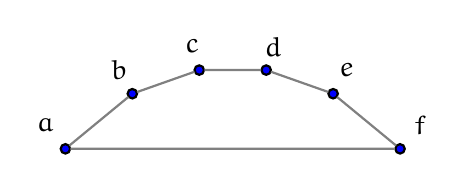
\begin{tikzpicture}[xscale=0.85]
\node at (-0.3,0.3) {$a$};
\node at (0.8,1) {$b$};
\node at (1.9,1.3) {$c$};
\node at (3.1,1.3) {$d$};
\node at (4.2,1) {$e$};
\node at (5.3,0.3) {$f$};
\node[draw,circle, thick, fill=blue, scale=0.3] (a) at (0,0) {};
\node[draw,circle, thick, fill=blue, scale=0.3] (b) at (1,0.7) {};
\node[draw,circle, thick, fill=blue, scale=0.3] (c) at (2,1) {};
\node[draw,circle, thick, fill=blue, scale=0.3] (d) at (3,1) {};
\node[draw,circle, thick, fill=blue, scale=0.3] (e) at (4,0.7) {};
\node[draw,circle, thick, fill=blue, scale=0.3] (f) at (5,0) {};
\draw[gray, thick] (a) -- (b) -- (c) -- (d) -- (e) -- (f) -- (a);
%\draw[gray] (a) -- (b) -- (c) -- (a);
%\draw[gray] (a) -- (c) -- (d) -- (a);
%\draw[gray] (a) -- (d) -- (e) -- (a);
%\draw[gray] (a) -- (e) -- (f) -- (a);
\end{tikzpicture}
\end{minipage}

\begin{minipage}{.47\textwidth}
\centering
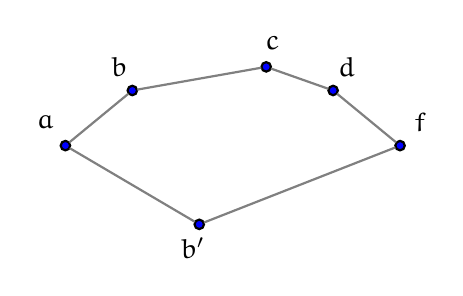
\begin{tikzpicture}[xscale=0.85]
\node at (-0.3,0.3) {$a$};
\node at (0.8,1) {$b$};
\node at (1.9,-1.3) {$b^{\prime}$};
\node at (3.1,1.3) {$c$};
\node at (4.2,1) {$d$};
\node at (5.3,0.3) {$f$};
\node[draw,circle, thick, fill=blue, scale=0.3] (a) at (0,0) {};
\node[draw,circle, thick, fill=blue, scale=0.3] (b) at (1,0.7) {};
\node[draw,circle, thick, fill=blue, scale=0.3] (c) at (2,-1) {};
\node[draw,circle, thick, fill=blue, scale=0.3] (d) at (3,1) {};
\node[draw,circle, thick, fill=blue, scale=0.3] (e) at (4,0.7) {};
\node[draw,circle, thick, fill=blue, scale=0.3] (f) at (5,0) {};
\draw[gray, thick] (a) -- (b) -- (d) -- (e) -- (f) -- (c) -- (a);
%\draw[gray] (a) -- (b) -- (d) -- (a);
%\draw[gray] (a) -- (c) -- (f) -- (a);
%\draw[gray] (a) -- (d) -- (e) -- (a);
%\draw[gray] (a) -- (e) -- (f) -- (a);
\end{tikzpicture}
\end{minipage}
\hfill
\begin{minipage}{.47\textwidth}
%\centering
$y_{a,f} \lor O_{a,b,c} \lor O_{b,c,d} \lor O_{c,d,f}$
$\overline{y_{a,f}} \lor \overline{O_{a,b^{\prime},f}}$

\end{minipage}


\vspace{-10pt}

\begin{minipage}{.47\textwidth}
%\centering
$z_{a,f} \lor O_{a,b,c} \lor O_{b,c,f}$\\
$\overline{z_{a,f}} \lor \overline{O_{a,b^{\prime},c^{\prime}}} \lor \overline{O_{b^{\prime},c^{\prime},f}}$\end{minipage}
\hfill
\begin{minipage}{.47\textwidth}
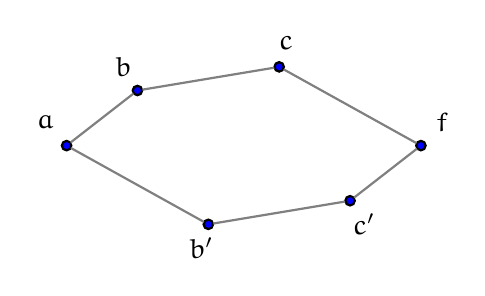
\begin{tikzpicture}[xscale=0.9]
\node at (-0.3,0.3) {$a$};
\node at (0.8,1) {$b$};
\node at (1.9,-1.3) {$b^{\prime}$};
\node at (3.1,1.3) {$c$};
\node at (4.2,-1) {$c^{\prime}$};
\node at (5.3,0.3) {$f$};
\node[draw,circle, thick, fill=blue, scale=0.3] (a) at (0,0) {};
\node[draw,circle, thick, fill=blue, scale=0.3] (b) at (1,0.7) {};
\node[draw,circle, thick, fill=blue, scale=0.3] (c) at (2,-1) {};
\node[draw,circle, thick, fill=blue, scale=0.3] (d) at (3,1) {};
\node[draw,circle, thick, fill=blue, scale=0.3] (e) at (4,-0.7) {};
\node[draw,circle, thick, fill=blue, scale=0.3] (f) at (5,0) {};
\draw[gray, thick] (a) -- (b) -- (d) -- (f) -- (e) -- (c) -- (a);
%\draw[gray] (a) -- (b) -- (d) -- (a);
%\draw[gray] (a) -- (c) -- (e) -- (a);
%\draw[gray] (a) -- (e) -- (f) -- (a);
%\draw[gray] (a) -- (d) -- (f) -- (a);
\end{tikzpicture}
\end{minipage}
}
\fi

\frame{
	\frametitle{Inside Variables}

\large

\medskip

We introduce \structure{inside variables} $I_{x;a,b,c}$ which are true
if and only if point $x$ is in the triangle $abc$ with $a < x < b$
or $b < x < c$.

\bigskip

%\begin{minipage}{.6\textwidth}
%${I_{x;a,b,c}} \lor \overline{O_{a,b,c}} \lor {O_{a,x,b}} \lor \overline{O_{x,b,c}} \lor \overline{O_{a,x,c}}$\\[3pt]
%$\overline{I_{x;a,b,c}} \lor \overline{O_{a,b,c}} \lor \overline{O_{a,x,b}}$\\[3pt]
%$\overline{I_{x;a,b,c}} \lor \overline{O_{a,b,c}} \lor O_{x,b,c}$\\[3pt]
%$\overline{I_{x;a,b,c}} \lor \overline{O_{a,b,c}} \lor O_{a,x,c}$\\[3pt]
%\end{minipage}
%%\hfill
%\begin{minipage}{.35\textwidth}
%\begin{tikzpicture}
%
%\node at (-0.3,-0.3) {$a$};
%\node at (2.3,-0.3) {$b$};
%\node at (3.3,1.8) {$c$};
%\node at (1.5,0.25) {$x$};
%\node[draw,circle, thick, fill=blue, scale=0.3] (a) at (0,0) {};
%\node[draw,circle, thick, fill=blue, scale=0.3] (b) at (2,0) {};
%\node[draw,circle, thick, fill=blue, scale=0.3] (c) at (3,1.5) {};
%\node[draw,circle, thick, fill=blue, scale=0.3] (x) at (1.5,0.5) {};
%\draw[gray] (a) -- (b) -- (c) -- (a);
%\end{tikzpicture}
%\end{minipage}
%
%\pause
%\bigskip
%
%\begin{minipage}{.6\textwidth}
%
%${I_{x;a,b,c}} \lor {O_{a,b,c}} \lor \overline{O_{a,x,b}} \lor O_{x,b,c} \lor O_{a,x,c}$\\[3pt]
%$\overline{I_{x;a,b,c}} \lor {O_{a,b,c}} \lor {O_{a,x,b}}$\\[3pt]
%$\overline{I_{x;a,b,c}} \lor {O_{a,b,c}} \lor \overline{O_{x,b,c}}$\\[3pt]
%$\overline{I_{x;a,b,c}} \lor {O_{a,b,c}} \lor \overline{O_{a,x,c}}$\\[3pt]
%\end{minipage}
%\begin{minipage}{.35\textwidth}
%\bigskip
%\begin{tikzpicture}
%
%\node at (-0.3,0.3) {$a$};
%\node at (2.3,0.3) {$b$};
%\node at (3.3,-1.8) {$c$};
%\node at (1.5,-0.25) {$x$};
%\node[draw,circle, thick, fill=blue, scale=0.3] (a) at (0,0) {};
%\node[draw,circle, thick, fill=blue, scale=0.3] (b) at (2,0) {};
%\node[draw,circle, thick, fill=blue, scale=0.3] (c) at (3,-1.5) {};
%\node[draw,circle, thick, fill=blue, scale=0.3] (x) at (1.5,-0.5) {};
%\draw[gray] (a) -- (b) -- (c) -- (a);
%\end{tikzpicture}
%\end{minipage}

\medskip
Four possible cases:
\medskip

{\normalsize
\begin{minipage}{.24\textwidth}
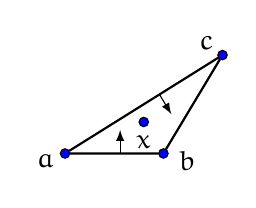
\begin{tikzpicture}
\node at (-0.25,-0.1) {$a$};
\node at (1.55,-0.1) {$b$};
\node at (1.8,1.4) {$c$};
\node at (1,0.15) {$x$};
\node[draw, circle, fill=blue, scale=0.3] (a) at (0,0) {};
\node[draw, circle, fill=blue, scale=0.3] (b) at (1.25,0) {};
\node[draw, circle, fill=blue, scale=0.3] (c) at (2,1.25) {};
\node[draw, circle, fill=blue, scale=0.3] (i) at (1,0.4) {};
\draw[thick] (a) -- (b) -- (c) -- (a);
\draw[-latex] (0.7,0) -- (0.7,0.3);
\draw[-latex] (1.2,0.75) -- (1.35,0.5);
\end{tikzpicture}
\end{minipage}
\hfil
\begin{minipage}{.24\textwidth}
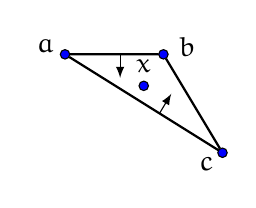
\begin{tikzpicture}
\node at (-0.25,0.1) {$a$};
\node at (1.55,0.1) {$b$};
\node at (1.8,-1.4) {$c$};
\node at (1,-0.15) {$x$};
\node[draw, circle, fill=blue, scale=0.3] (a) at (0,0) {};
\node[draw, circle, fill=blue, scale=0.3] (b) at (1.25,0) {};
\node[draw, circle, fill=blue, scale=0.3] (c) at (2,-1.25) {};
\node[draw, circle, fill=blue, scale=0.3] (i) at (1,-0.4) {};
\draw[thick] (a) -- (b) -- (c) -- (a);
\draw[-latex] (0.7,0) -- (0.7,-0.3);
\draw[-latex] (1.2,-0.75) -- (1.35,-0.5);
\end{tikzpicture}
\end{minipage}
\hfil
\begin{minipage}{.24\textwidth}
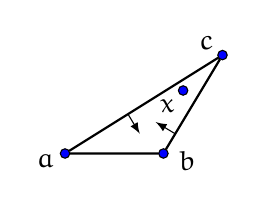
\begin{tikzpicture}
\node at (-0.25,-0.1) {$a$};
\node at (1.55,-0.1) {$b$};
\node at (1.8,1.4) {$c$};
\node at (1.3,0.6) {$x$};
\node[draw, circle, fill=blue, scale=0.3] (a) at (0,0) {};
\node[draw, circle, fill=blue, scale=0.3] (b) at (1.25,0) {};
\node[draw, circle, fill=blue, scale=0.3] (c) at (2,1.25) {};
\node[draw, circle, fill=blue, scale=0.3] (i) at (1.5,0.8) {};
\draw[thick] (a) -- (b) -- (c) -- (a);
\draw[-latex] (0.8,0.5) -- (0.95,0.25);
\draw[-latex] (1.40,0.25) -- (1.15,0.4);
\end{tikzpicture}
\end{minipage}
\hfil
\begin{minipage}{.24\textwidth}
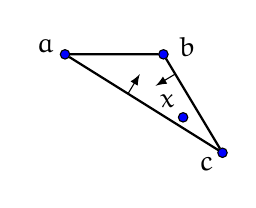
\begin{tikzpicture}
\node at (-0.25,0.1) {$a$};
\node at (1.55,0.1) {$b$};
\node at (1.8,-1.4) {$c$};
\node at (1.3,-0.6) {$x$};
\node[draw, circle, fill=blue, scale=0.3] (a) at (0,-0) {};
\node[draw, circle, fill=blue, scale=0.3] (b) at (1.25,-0) {};
\node[draw, circle, fill=blue, scale=0.3] (c) at (2,-1.25) {};
\node[draw, circle, fill=blue, scale=0.3] (i) at (1.5,-0.8) {};
\draw[thick] (a) -- (b) -- (c) -- (a);
\draw[-latex] (0.8,-0.5) -- (0.95,-0.25);
\draw[-latex] (1.40,-0.25) -- (1.15,-0.4);
\end{tikzpicture}
\end{minipage}
}

\pause
\bigskip
\medskip

The left two cases with $a < x < b$:\\[-20pt]
\begin{equation*}
\!\!\!\!\!\!\!\!\!\!\!\! I_{x;abc} \leftrightarrow \Big(\big(O_{abc} \rightarrow (\overline{O_{axb}} ~\land~ O_{axc})\big)~\land~ 
               \big(\overline{O_{abc}} \rightarrow (O_{axb} ~\land~ \overline{O_{axc}})\big)\Big)
\end{equation*}



The right two cases with $b < x < c$:\\[-20pt]
\begin{equation*}
\!\!\!\!\!\!\!\!\!\!\!\! I_{x;abc} \leftrightarrow \Big(\big(O_{abc} \rightarrow ({O_{axc}} ~\land~ \overline{O_{bxc}})\big)~\land~ 
               \big(\overline{O_{abc}} \rightarrow (\overline{O_{axc}} ~\land~ {O_{bxc}})\big)\Big)
%\insidep{i}{a}{b}{c} \leftrightarrow \Big(\big(\orientp{a}{b}{c} \rightarrow (\orientp{a}{i}{c} \land \orientn{b}{i}{c})\big) \land \big(\orientn{a}{b}{c} \rightarrow (\orientn{a}{i}{c} \land \orientp{b}{i}{c})\big)\Big)
\end{equation*}

%  printf ("%i %i %i 0\n", -d,  t, -abx);
%  printf ("%i %i %i 0\n", -d,  t, -bcx);
%  printf ("%i %i %i 0\n", -d,  t, -acx);
%
%  printf ("%i %i %i 0\n", -d, -t,  abx);
%  printf ("%i %i %i 0\n", -d, -t,  bcx);
%  printf ("%i %i %i 0\n", -d, -t,  acx);
%
%#ifdef BLOCKED
%  printf ("%i %i %i %i %i 0\n", d,  t,  abx,  bcx,  acx);
%  printf ("%i %i %i %i %i 0\n", d, -t, -abx, -bcx, -acx);
%#endif

}

\frame{
	\frametitle{Hole Variables}
	
\large

We introduce \structure{hole variables} $H_{abc}$ which are true
if and only if no points occur with the triangle $abc$ with $a < b < c$.

\medskip

\[
H_{abc} \lor \bigvee_{a < x < c} {I_{x;abc}}
\]

\[
\bigwedge_{a < x < c} \overline{H_{abc}} \lor \overline{I_{x;abc}}~~~~~~~\mathrm{(redundant)}
\]

\bigskip
\pause

Simple $6$-hole encoding:

\begin{center}
$\bigvee_{a,b,c \in X} \overline{H_{abc}}$~~~~$\forall~X \subset S$ with $|X| = 6$
\end{center}

}

\iffalse
\frame{
	\frametitle{$k$-Hole Encoding}

\large

\bigskip

\begin{minipage}{.52\textwidth}
%\centering
$O_{a,b,c} \lor O_{b,c,d} \lor O_{c,d,e} \lor O_{d,e,f}~\lor$\\[3pt]
$\overline{H_{a,b,c}} \lor \overline{H_{a,c,d}} \lor \overline{H_{a,d,e}} \lor \overline{H_{a,e,f}}$\\
\end{minipage}
\hfill
\begin{minipage}{.45\textwidth}
\centering
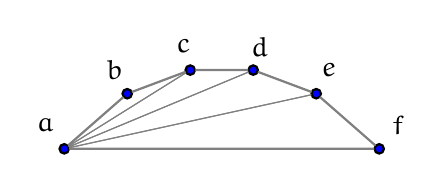
\begin{tikzpicture}[xscale=0.8]
\node at (-0.3,0.3) {$a$};
\node at (0.8,1) {$b$};
\node at (1.9,1.3) {$c$};
\node at (3.1,1.3) {$d$};
\node at (4.2,1) {$e$};
\node at (5.3,0.3) {$f$};
\node[draw,circle, thick, fill=blue, scale=0.3] (a) at (0,0) {};
\node[draw,circle, thick, fill=blue, scale=0.3] (b) at (1,0.7) {};
\node[draw,circle, thick, fill=blue, scale=0.3] (c) at (2,1) {};
\node[draw,circle, thick, fill=blue, scale=0.3] (d) at (3,1) {};
\node[draw,circle, thick, fill=blue, scale=0.3] (e) at (4,0.7) {};
\node[draw,circle, thick, fill=blue, scale=0.3] (f) at (5,0) {};
\draw[gray, thick] (a) -- (b) -- (c) -- (d) -- (e) -- (f) -- (a);
\draw[gray] (a) -- (b) -- (c) -- (a);
\draw[gray] (a) -- (c) -- (d) -- (a);
\draw[gray] (a) -- (d) -- (e) -- (a);
\draw[gray] (a) -- (e) -- (f) -- (a);
\end{tikzpicture}
\end{minipage}

\begin{minipage}{.45\textwidth}
\centering
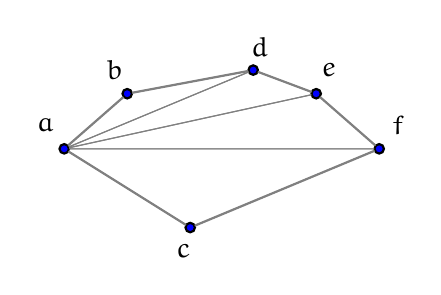
\begin{tikzpicture}[xscale=0.8]
\node at (-0.3,0.3) {$a$};
\node at (0.8,1) {$b$};
\node at (1.9,-1.3) {$c$};
\node at (3.1,1.3) {$d$};
\node at (4.2,1) {$e$};
\node at (5.3,0.3) {$f$};
\node[draw,circle, thick, fill=blue, scale=0.3] (a) at (0,0) {};
\node[draw,circle, thick, fill=blue, scale=0.3] (b) at (1,0.7) {};
\node[draw,circle, thick, fill=blue, scale=0.3] (c) at (2,-1) {};
\node[draw,circle, thick, fill=blue, scale=0.3] (d) at (3,1) {};
\node[draw,circle, thick, fill=blue, scale=0.3] (e) at (4,0.7) {};
\node[draw,circle, thick, fill=blue, scale=0.3] (f) at (5,0) {};
\draw[gray, thick] (a) -- (b) -- (d) -- (e) -- (f) -- (c) -- (a);
\draw[gray] (a) -- (b) -- (d) -- (a);
\draw[gray] (a) -- (c) -- (f) -- (a);
\draw[gray] (a) -- (d) -- (e) -- (a);
\draw[gray] (a) -- (e) -- (f) -- (a);
\end{tikzpicture}
\end{minipage}
\hfill
\begin{minipage}{.52\textwidth}
$O_{a,b,d} \lor O_{b,d,e} \lor O_{d,e,f} \lor \overline{O_{a,c,f}}~\lor$\\[3pt]
$\overline{H_{a,b,d}} \lor \overline{H_{a,d,e}} \lor \overline{H_{a,e,f}} \lor \overline{H_{a,c,f}}$
\end{minipage}


\vspace{-10pt}

\begin{minipage}{.52\textwidth}
$O_{a,b,d} \lor O_{b,d,f} \lor \overline{O_{a,c,e}} \lor \overline{O_{c,e,f}}~\lor$
$\overline{H_{a,b,d}} \lor \overline{H_{a,d,f}} \lor \overline{H_{a,c,e}} \lor \overline{H_{a,e,f}}$

\end{minipage}
\hfill
\begin{minipage}{.45\textwidth}
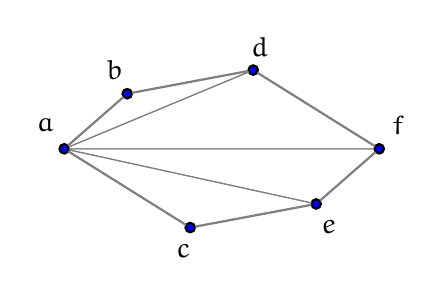
\begin{tikzpicture}[xscale=0.8]
\node at (-0.3,0.3) {$a$};
\node at (0.8,1) {$b$};
\node at (1.9,-1.3) {$c$};
\node at (3.1,1.3) {$d$};
\node at (4.2,-1) {$e$};
\node at (5.3,0.3) {$f$};
\node[draw,circle, thick, fill=blue, scale=0.3] (a) at (0,0) {};
\node[draw,circle, thick, fill=blue, scale=0.3] (b) at (1,0.7) {};
\node[draw,circle, thick, fill=blue, scale=0.3] (c) at (2,-1) {};
\node[draw,circle, thick, fill=blue, scale=0.3] (d) at (3,1) {};
\node[draw,circle, thick, fill=blue, scale=0.3] (e) at (4,-0.7) {};
\node[draw,circle, thick, fill=blue, scale=0.3] (f) at (5,0) {};
\draw[gray, thick] (a) -- (b) -- (d) -- (f) -- (e) -- (c) -- (a);
\draw[gray] (a) -- (b) -- (d) -- (a);
\draw[gray] (a) -- (c) -- (e) -- (a);
\draw[gray] (a) -- (e) -- (f) -- (a);
\draw[gray] (a) -- (d) -- (f) -- (a);
\end{tikzpicture}
\end{minipage}
}
\fi

\frame{
	\frametitle{$6$-Hole Encoding: One Triangle-is-Empty Check Required}

\large

Trusted $6$-hole encoding uses $O(n^6)$ clauses with \structure{20 literals}:
\begin{center}
$\bigvee_{a,b,c \in X} \overline{H_{abc}}$~~~~$\forall~X \subset S$ with $|X| = 6$
\end{center}

\begin{example}

\begin{minipage}{.6\textwidth}
\smallskip
Consider an assignment with
\begin{itemize}
\item $O_{abd} = 0$ and $O_{bdf} = 0$
\item $O_{ace} = 1$ and $O_{cef} = 1$
\only<1>{\vspace{35pt}}
\only<2->{
\item $H_{ade} = 1$}
\end{itemize}
\only<2->{
This implies the \structure{existence of a $6$-hole}!}
\end{minipage}
\begin{minipage}{.38\textwidth}
\begin{tikzpicture}[scale=1.2]
\node at (0,0.4) {$a$};
\node at (0.8,1) {$b$};
\node at (1.9,-1.3) {$c$};
\node at (3.1,1) {$d$};
\node at (3.1,-1) {$e$};
\node at (3.6,0.3) {$f$};

% only works with coordinates
\only<2->{
\filldraw[draw=structure, thick, fill=structure!30!white]
(0,0) -- (2.8,0.7) -- (3.1,-0.5) -- cycle;}

\node[draw,circle, fill=blue, scale=0.3] (a) at (0,0) {};
\node[draw,circle, fill=blue, scale=0.3] (b) at (1,0.8) {};
\node[draw,circle, fill=blue, scale=0.3] (c) at (2,-0.9) {};
\node[draw,circle, fill=blue, scale=0.3] (d) at (2.8,0.7) {};
\node[draw,circle, fill=blue, scale=0.3] (e) at (3.1,-0.5) {};
\node[draw,circle, fill=blue, scale=0.3] (f) at (3.5,0) {};
\draw[black, thick] (a) -- (b) -- (d) -- (f) -- (e) -- (c) -- (a);
\end{tikzpicture}
\end{minipage}

\pause
\pause
\bigskip

Clause to prevent this: $O_{abd} \lor O_{bdf} \lor \overline{O_{ace}} \lor \overline{O_{cef}} \lor \overline{H_{ade}}$\!\!\!\!\!\!\!\!


\end{example}

\pause 
\bigskip

\structure{This encoding is 16 times larger, but much easier to solve}


}
%\frame{
%	\frametitle{$k$-Hole Encoding (I)}
%
%\large
%
%Simple $6$-hole encoding with $O(n^6)$ clauses with \structure{20 literals}:
%\begin{center}
%$(\bigvee_{a,b,c \in X} \overline{H_{a,b,c}})$~~~~$\forall~X \subset S$ with $|X| = 6$
%\end{center}
%
%\medskip
%\pause
%
%Shorter clauses, thus \structure{more propagation}, but still $O(n^6)$
%
%\begin{minipage}{.52\textwidth}
%$O_{a,b,d} \lor O_{b,d,f} \lor \overline{O_{a,c,e}} \lor \overline{O_{c,e,f}}~\lor$
%$\overline{H_{a,b,d}} \lor \overline{H_{a,d,f}} \lor \overline{H_{a,c,e}} \lor \overline{H_{a,e,f}}$
%\end{minipage}
%\hfill
%\begin{minipage}{.45\textwidth}
%\begin{tikzpicture}[xscale=0.8]
%\node at (-0.3,0.3) {$a$};
%\node at (0.8,1) {$b$};
%\node at (1.9,-1.3) {$c$};
%\node at (3.1,1.3) {$d$};
%\node at (4.2,-1) {$e$};
%\node at (5.3,0.3) {$f$};
%\node[draw,circle, thick, fill=blue, scale=0.3] (a) at (0,0) {};
%\node[draw,circle, thick, fill=blue, scale=0.3] (b) at (1,0.7) {};
%\node[draw,circle, thick, fill=blue, scale=0.3] (c) at (2,-1) {};
%\node[draw,circle, thick, fill=blue, scale=0.3] (d) at (3,1) {};
%\node[draw,circle, thick, fill=blue, scale=0.3] (e) at (4,-0.7) {};
%\node[draw,circle, thick, fill=blue, scale=0.3] (f) at (5,0) {};
%\draw[gray, thick] (a) -- (b) -- (d) -- (f) -- (e) -- (c) -- (a);
%\draw[gray] (a) -- (b) -- (d) -- (a);
%\draw[gray] (a) -- (c) -- (e) -- (a);
%\draw[gray] (a) -- (e) -- (f) -- (a);
%\draw[gray] (a) -- (d) -- (f) -- (a);
%\end{tikzpicture}
%\end{minipage}
%
%\medskip
%\pause
%
%\structure{Auxiliary variables} make an $O(n^4)$ clauses encoding possible
%\begin{eqnarray*}
%&\!\!\!\!\!\!\!\!\!\!\!\!\!\! x_{a,f} \lor O_{a,b,d} \lor O_{b,d,f} \lor \overline{H_{a,b,d}} \lor \overline{H_{a,d,f}}&\mathrm{with~}a < b < d < f\\
%&\!\!\!\!\!\!\!\!\!\!\!\!\!\! \overline{x_{a,f}} \lor \overline{O_{a,c,e}} \lor \overline{O_{c,e,f}} \lor \overline{H_{a,c,e}} \lor \overline{H_{a,e,f}}&\mathrm{with~}a < c < e < f
%\end{eqnarray*}
%
%}


\frame{
	\frametitle{$k$-Hole Encoding Using $O(n^4)$ Clauses}

\large

Shorter clauses, thus \structure{more propagation}, but still $O(n^6)$

\bigskip

\begin{example}

\begin{minipage}{.6\textwidth}
\smallskip
Introduce $O(n^3)$ auxiliary variables: 
\begin{itemize}
\item $A_{acd}$: a $4$-gon \structure{above} the line $ad$\\[5pt]
        $\overline{O_{abc}} \land \overline{O_{bcd}} \rightarrow A_{acd}$
\item $B_{ac'd}$: a $4$-gon \structure{below} the line $ad$\\[5pt]
        ${O_{ab'c'}} \land {O_{b'c'd}} \rightarrow B_{ac'd}$
\item Combine them to \structure{block} $6$-holes\\[5pt]
         $\overline{A_{acd}} \lor \overline{B_{ac'd}} \lor \overline{H_{acc'}}$
\end{itemize}
\end{minipage}
\begin{minipage}{.38\textwidth}
\begin{tikzpicture}[scale=1.2]
\node at (0,0.4) {$a$};
\node at (0.8,1) {$b$};
\node at (1.9,-1.3) {$b'$};
\node at (3.1,1) {$c$};
\node at (3.1,-1) {$c'$};
\node at (3.6,0.3) {$d$};

% only works with coordinates
\filldraw[draw=structure, thick, fill=structure!30!white]
(0,0) -- (2.8,0.7) -- (3.1,-0.5) -- cycle;

\node[draw,circle, fill=blue, scale=0.3] (a) at (0,0) {};
\node[draw,circle, fill=blue, scale=0.3] (b) at (1,0.8) {};
\node[draw,circle, fill=blue, scale=0.3] (c) at (2,-0.9) {};
\node[draw,circle, fill=blue, scale=0.3] (d) at (2.8,0.7) {};
\node[draw,circle, fill=blue, scale=0.3] (e) at (3.1,-0.5) {};
\node[draw,circle, fill=blue, scale=0.3] (f) at (3.5,0) {};
\draw[black, thick] (a) -- (b) -- (d) -- (f) -- (e) -- (c) -- (a);

\draw[structure, very thick] (a) -- (f);
\end{tikzpicture}
\end{minipage}

\end{example}


\bigskip

This reduces the size of the encoding to $O(n^4)$ clauses

}

%\frame{
%	\frametitle{$k$-Hole Encoding (II)}
%
%\large
%
%Shorter clauses, thus \structure{more propagation}, but still $O(n^6)$
%
%\bigskip
%
%\begin{minipage}{.52\textwidth}
%%\centering
%\medskip
%$O_{a,b,c} \lor O_{b,c,d} \lor O_{c,d,e} \lor O_{d,e,f}~\lor$\\[3pt]
%$\overline{H_{a,b,c}} \lor \overline{H_{a,c,d}} \lor \overline{H_{a,d,e}} \lor \overline{H_{a,e,f}}$\\
%\end{minipage}
%\hfill
%\begin{minipage}{.45\textwidth}
%\centering
%\begin{tikzpicture}[xscale=0.8]
%\node at (-0.3,0.3) {$a$};
%\node at (0.8,1) {$b$};
%\node at (1.9,1.3) {$c$};
%\node at (3.1,1.3) {$d$};
%\node at (4.2,1) {$e$};
%\node at (5.3,0.3) {$f$};
%\node[draw,circle, thick, fill=blue, scale=0.3] (a) at (0,0) {};
%\node[draw,circle, thick, fill=blue, scale=0.3] (b) at (1,0.7) {};
%\node[draw,circle, thick, fill=blue, scale=0.3] (c) at (2,1) {};
%\node[draw,circle, thick, fill=blue, scale=0.3] (d) at (3,1) {};
%\node[draw,circle, thick, fill=blue, scale=0.3] (e) at (4,0.7) {};
%\node[draw,circle, thick, fill=blue, scale=0.3] (f) at (5,0) {};
%\draw[gray, thick] (a) -- (b) -- (c) -- (d) -- (e) -- (f) -- (a);
%\draw[gray] (a) -- (b) -- (c) -- (a);
%\draw[gray] (a) -- (c) -- (d) -- (a);
%\draw[gray] (a) -- (d) -- (e) -- (a);
%\draw[gray] (a) -- (e) -- (f) -- (a);
%\end{tikzpicture}
%\end{minipage}
%
%\bigskip
%\bigskip
%\pause
%
%\structure{Auxiliary variables} make an $O(n^4)$ clauses encoding possible
%\begin{eqnarray*}
%&\!\!\!\!\!\!\!\!\!\!\!\!\!\! y_{a,c,d} \lor O_{a,b,c} \lor O_{b,c,d} \lor \overline{H_{a,b,c}} \lor \overline{H_{a,c,d}}&\mathrm{with~}a < b < c < d\\
%&\!\!\!\!\! z_{a,d,e} \lor \overline{O_{c,d,e}} \lor \overline{H_{a,d,e}} \lor \overline{y_{a,c,d}}&\mathrm{with~}a < c < d < e\\
%&\!\!\!\!\!  \overline{O_{d,e,f}} \lor \overline{H_{a,e,f}} \lor \overline{z_{a,d,e}}&\mathrm{with~}a < d < e < f
%\end{eqnarray*}
%
%
%
%
%}


%\iffalse
\frame{
	\frametitle{Symmetry Breaking: Sorted \& Rotated Around Point 1}

   \newcommand{\xa}{0}  \newcommand{\ya}{0}
   \newcommand{\xb}{1.5}  \newcommand{\yb}{0.2}
   \newcommand{\xc}{2.5}  \newcommand{\yc}{1.8}
   \newcommand{\xd}{1.3}  \newcommand{\yd}{1.9}
   \newcommand{\xe}{0.5}  \newcommand{\ye}{1.7}
   
   \newcommand{\ep}{0.5}
      
    \newcommand{\x}{6}
	
    \begin{minipage}{.48\textwidth}
    \centering
    \resizebox{!}{80pt}{
    \begin{tikzpicture}
    
    \draw (-0.5,0) -- (3,0);
    \draw (0,-1.5) -- (0,1.5);
    
%    \begin{scope}
%    \vertex{0}{0}{\x}; \node at (0,0) {\textcolor{white}{1}};
%    \vertex{0.7}{0.8}{\x}; \node at (0.7,0.8) {\textcolor{white}{5}};
%    \vertex{0.9}{-1}{\x}; \node at (0.9,-1) {\textcolor{white}{2}};
%    \vertex{1.2}{0.7}{\x}; \node at (1.2,0.7) {\textcolor{white}{4}};
%    \vertex{1.5}{-0.9}{\x}; \node at (1.5,-0.9) {\textcolor{white}{3}};
%    \end{scope}
     \begin{scope}[xscale=0.5]
        \begin{scope}[rotate=-45]
      \vertex{\xa}{\ya}{\x}; \node at (\xa,\ya) {\textcolor{white}{1}};
      \vertex{\xb}{\yb}{\x}; \node at (\xb,\yb) {\textcolor{white}{2}};
      \vertex{\xc}{\yc}{\x}; \node at (\xc,\yc) {\textcolor{white}{3}};
      \vertex{\xd}{\yd}{\x}; \node at (\xd,\yd) {\textcolor{white}{4}};
      \vertex{\xe}{\ye}{\x}; \node at (\xe,\ye) {\textcolor{white}{5}};
      \end{scope}
    \end{scope}
  
    \vertex{0}{0}{\x}; \node at (0,0) {\textcolor{white}{1}};
    \vertex{0.61}{-0.92}{\x}; \node at (0.61,-0.92) {\textcolor{white}{2}};
    \vertex{1.51}{-0.495}{\x}; \node at (1.51,-0.495) {\textcolor{white}{3}};
    \vertex{1.13}{0.42}{\x}; \node at (1.13,0.42) {\textcolor{white}{4}};
    \vertex{0.79}{0.85}{\x}; \node at (0.79,0.85) {\textcolor{white}{5}};

    
    \end{tikzpicture}}
    
    
    \smallskip
    place leftmost point at origin
    \phantom{place leftmost point at origin}
    \end{minipage}
    \begin{minipage}{.48\textwidth}
    \centering
    \resizebox{!}{80pt}{
    \begin{tikzpicture}
    
    \draw (-0.5,0) -- (3,0);
    \draw (0,-1.5) -- (0,1.5);
    \draw (0,0) -- (1.5,-1.5);
    \draw (0,0) -- (1.5,1.5);
    
    \begin{scope}[rotate=-45]
    \vertex{\xa}{\ya}{\x}; \node at (\xa,\ya) {\textcolor{white}{1}};
    \vertex{\xb}{\yb}{\x}; \node at (\xb,\yb) {\textcolor{white}{2}};
    \vertex{\xc}{\yc}{\x}; \node at (\xc,\yc) {\textcolor{white}{3}};
    \vertex{\xd}{\yd}{\x}; \node at (\xd,\yd) {\textcolor{white}{4}};
    \vertex{\xe}{\ye}{\x}; \node at (\xe,\ye) {\textcolor{white}{5}};
%    \vertex{0}{0}{\x}; \node at (0,0) {\textcolor{white}{1}};
%    \vertex{1.4}{0.8}{\x}; \node at (1.4,0.8) {\textcolor{white}{5}};
%    \vertex{1.8}{-1}{\x}; \node at (1.8,-1) {\textcolor{white}{2}};
%    \vertex{2.4}{0.7}{\x}; \node at (2.4,0.7) {\textcolor{white}{4}};
%    \vertex{3}{-0.9}{\x}; \node at (3,-0.9) {\textcolor{white}{3}};
    \end{scope}
    
    \end{tikzpicture}}
    \smallskip
    
    stretch points to the right to be\\[-1pt] within $y=x$ and $y=-x$
    \end{minipage}
    
    \bigskip
    
        \begin{minipage}{.48\textwidth}
    \centering
    \resizebox{!}{80pt}{
    \begin{tikzpicture}
    
     \draw (-0.5,0) -- (3,0);
     \draw (0,-0.5) -- (0,2.5);
    
    \vertex{\xa}{\ya}{\x}; \node at (\xa,\ya) {\textcolor{white}{1}};
    \vertex{\xb}{\yb}{\x}; \node at (\xb,\yb) {\textcolor{white}{2}};
    \vertex{\xc}{\yc}{\x}; \node at (\xc,\yc) {\textcolor{white}{3}};
    \vertex{\xd}{\yd}{\x}; \node at (\xd,\yd) {\textcolor{white}{4}};
    \vertex{\xe}{\ye}{\x}; \node at (\xe,\ye) {\textcolor{white}{5}};

    
%    \begin{scope}[rotate=45]
%    \vertex{0}{0}{\x}; \node at (0,0) {\textcolor{white}{1}};
%    \vertex{1.4}{0.8}{\x}; \node at (1.4,0.8) {\textcolor{white}{5}};
%    \vertex{1.8}{-1}{\x}; \node at (1.8,-1) {\textcolor{white}{2}};
%    \vertex{2.4}{0.7}{\x}; \node at (2.4,0.7) {\textcolor{white}{4}};
%    \vertex{3}{-0.9}{\x}; \node at (3,-0.9) {\textcolor{white}{3}};
%    \end{scope}
    
    \end{tikzpicture}}
    
    rotate by 45 degrees
    
    \end{minipage}
    \begin{minipage}{.48\textwidth}
    \centering
    
    
    \resizebox{!}{80pt}{\begin{tikzpicture}
    
     \draw (-0.5,0) -- (3,0);
     \draw (0,-0.5) -- (0,2.5);
    
%    \vertex{0}{0}{\x}; \node at (0,0) {\textcolor{white}{1}};
%    \vertex{1.8}{0.4}{\x}; \node at (1.8,0.4) {\textcolor{white}{2}};
%    \vertex{2.5}{1.2}{\x}; \node at (2.5,1.2) {\textcolor{white}{3}};
%    \vertex{1}{2.1}{\x}; \node at (1,2.1) {\textcolor{white}{4}};
%    \vertex{0.3}{1.4}{\x}; \node at (0.3,1.4) {\textcolor{white}{5}};
    
      \vertex{{\ya/(\xa+\ep)}}{{1/(\xa+\ep)}}{\x}; \node at ({\ya/(\xa+\ep)},{1/(\xa+\ep)}) {\textcolor{white}{1}};
      \vertex{{\yb/(\xb+\ep)}}{{1/(\xb+\ep)}}{\x}; \node at ({\yb/(\xb+\ep)},{1/(\xb+\ep)}) {\textcolor{white}{2}};
      \vertex{{\yc/(\xc+\ep)}}{{1/(\xc+\ep)}}{\x}; \node at ({\yc/(\xc+\ep)},{1/(\xc+\ep)}) {\textcolor{white}{3}};
      \vertex{{\yd/(\xd+\ep)}}{{1/(\xd+\ep)}}{\x}; \node at ({\yd/(\xd+\ep)},{1/(\xd+\ep)}) {\textcolor{white}{4}};
      \vertex{{\ye/(\xe+\ep)}}{{1/(\xe+\ep)}}{\x}; \node at ({\ye/(\xe+\ep)},{1/(\xe+\ep)}) {\textcolor{white}{5}};
    
%    \vertex{0}{5}{\x}; \node at (0,5) {\textcolor{white}{1}};
%    \vertex{0.4/1.8}{1/1.8}{\x}; \node at (0.4/1.8,1/1.8) {\textcolor{white}{2}};
%    \vertex{1.2/2.5}{1/2.5}{\x}; \node at (1.2/2.5,1/2.5) {\textcolor{white}{3}};
%    \vertex{2.1/1}{1/1}{\x}; \node at (2.1/1,1/1) {\textcolor{white}{4}};
%    \vertex{1.4/0.3}{1/0.3}{\x}; \node at (1.4/0.3,1/0.3) {\textcolor{white}{5}};
%    \begin{scope}
%    \vertex{0}{0}{\x}; \node at (0,0) {\textcolor{white}{1}};
%    \vertex{1.4}{1.2}{\x}; \node at (1.4,1.2) {\textcolor{white}{5}};
%    \vertex{3}{-1}{\x}; \node at (3,-1) {\textcolor{white}{2}};
%    \vertex{4}{0.7}{\x}; \node at (4,0.7) {\textcolor{white}{3}};
%    \vertex{5}{1.3}{\x}; \node at (5,1.3) {\textcolor{white}{4}};
%    \end{scope}
    
    \end{tikzpicture}}
    
    projective transformation $(x,y) \mapsto (y/(x+\epsilon),1/(x+\epsilon))$
    \end{minipage}

}
%\fi

\frame{
	\frametitle{Realizability Constraints}

\large

Under the assumption that points are sorted from left to right
%$\forall a < b < c < d$: ``at most one sign change''


\begin{center}
\begin{minipage}{.5\textwidth}
\begin{tikzpicture}[scale=1.3]
\newcommand{\x}{1.5}
\vertex{.32}{6.56}{\x};
\vertex{1.12}{6.24}{\x};
\vertex{1.92}{6.72}{\x};
  \draw[shift={(.32, 6.56)}, scale=3.414]
    (0, 0)
     -- (.80, -.32);
  \draw[shift={(1.12, 6.24001)}, scale=2.5322]
    (0, 0)
     -- (.80, .48);
  \draw[shift={(3.5081, 6.8788)}, scale=1.9926]
    (0, 0)
     -- (-1.60, -.16);
\only<4->{
\vertexc{2.72}{5.12}{\x}{xorange};}
\only<3->{
\vertexc{2.72}{6.24}{\x}{cyan};}
\only<2->{
\vertexc{2.72}{7.04}{\x}{xgreen};}
\vertexc{2.72}{7.68}{\x}{structure};
  \node
     at (.16, 6.24) {$a$};
  \node
     at (.96, 5.92) {$b$};
  \node
     at (1.76, 6.88) {$c$};
  \node
     at (2.72, 8.5) {$d$};
  \node
     at (2.72, 5) {$~$};
\end{tikzpicture}

\end{minipage}
\begin{minipage}{.4\textwidth}


\begin{tabular}{cccc}
\toprule
$O_{abc}$ & $O_{abd}$ & $O_{acd}$ & $O_{bcd}$\\
\midrule
\textcolor{structure}{$+$} & \textcolor{structure}{$+$} & \textcolor{structure}{$+$} & \textcolor{structure}{$+$}\\
\pause
\textcolor{xgreen}{$+$} & \textcolor{xgreen}{$+$} & \textcolor{xgreen}{$+$} & \textcolor{xgreen}{$-$}\\
\pause
\textcolor{cyan}{$+$} & \textcolor{cyan}{$+$} & \textcolor{cyan}{$-$} & \textcolor{cyan}{$-$}\\
\pause
\textcolor{xorange}{$+$} & \textcolor{xorange}{$-$} & \textcolor{xorange}{$-$} & \textcolor{xorange}{$-$}\\
\pause
$-$ & $-$ & $-$ & $-$\\
$-$ & $-$ & $-$ & $+$\\
$-$ & $-$ & $+$ & $+$\\
$-$ & $+$ & $+$ & $+$\\
\bottomrule
\end{tabular}

\end{minipage}
\end{center}

Block multiple sign changes with $\Theta(n^4)$ (ternary) clauses \textcolor{xgreen}{[Felsner \& Weil ’01]}


}

\section{Results}
\frame{\Large \tableofcontents[currentsection]}


\frame{
	\frametitle{Impact of the Encoding}

\large

Four different encodings of a random subproblem
\begin{itemize}
\item $T$: the trusted encoding
\item $O_1$: the explicit encoding with a single empty triangle
\item $O_2$: reduce the size of $O_1$ with auxiliary variables to $O(n^4)$
\item $O_3$: $O_2$ without redundant clauses
% \item $O_4$:   
\end{itemize}

\bigskip
\bigskip

\begin{tabular}{c@{~~}r@{~~}r@{~~}r@{~~}r@{~~}r@{~~}r@{~~}c}
\toprule
$\Gamma$ & $\#$var~ & $\#$clause~ & $\#$conflict & $\#$propagation & time (s) \\
\midrule
$T$     & 62\,930 & 1\,171\,942 & 1\,082\,569 & 1\,338\,662\,627 & 243.07\\
$O_1$ & 62\,930 & 5\,823\,078 &    228\,838 &     282\,774\,472 & 136.20\\
$O_2$ & 75\,110 &     667\,005 &    211\,272 &      343\,388\,591 &  45.49\\
$O_3$ & 75\,110 &     436\,047 &    234\,755 &      340\,387\,692 &  39.46\\
% $O_4$ & 75\,110 &     444\,238 &    234\,587 &      342\,904\,580 &  39.41\\
\bottomrule
\end{tabular}

}


\frame{
	\frametitle{Comparison to Existing Work}

\large

Szekeres and Peters (2006) solved $g(6) =17$ in 63 CPU days\!\!\!\!\!
\begin{itemize}
\item Roughly 40 CPU hours on today's hardware
\item \url{https://www.cpubenchmark.net/year-on-year.html}
\end{itemize}

\bigskip

SAT solving, using the same abstraction, is much faster
\begin{itemize}
\item The independent SAT-approaches by Marić and Scheucher required a few CPU hours
\item Their encodings consist of $O(n^k)$ clauses
\end{itemize}

\bigskip

Our $O(n^4)$ encoding for $k$-gons and $k$-holes is even faster
\begin{itemize}
\item $g(6) =17$ can be solved in 10 CPU seconds
\item Roughly 4 orders of magnitude faster than to original proof
\end{itemize} 


}


\frame{
	\frametitle{Problem Partitioning}

\large

%The interesting problems are too hard for a single CPU
%
%\bigskip

Partitioning to split the problem into easier subproblems
\begin{itemize}
\item Original problem UNSAT iff all subproblems UNSAT
\item Split on variables $O_{a,a+1,a+2}$ starting from the middle
\item One parameter: the length $\ell$, roughly $1.83^\ell$ cubes
\item Tested on: 24 points contain $6$-hole \structure{or} $7$-gon
\end{itemize}

\medskip

\centering

\begin{tabular}{@{~~~}r@{~~~}r@{~~~}r@{~~~}r@{~~~}r@{~~~}r@{~~~}c}
\toprule
 $\ell$~ & $\#$cubes & avg time (s) & max time (s) & total (h)\\
\midrule
21 & 312\,418 & 6.99~~~  & 66.86~~~ & 606.55~~~\\
19 & 89\,384 & 13.61~~~ & 123.70~~~ & 337.96~~~\\
17 & 25\,663 & 34.29~~~ & 293.10~~~ & 244.50~~~\\
15 & 7393 & 112.61~~~ & 949.50~~~ & {\bf 231.27}~~~\\
13 & 2149 & 431.26~~~ & 3\,347.59~~~ & 257.44~~~\\
11 & 629 & 1\,847.46~~~ & 11\,844.05~~~ & 322.79~~~\\
9 & 188 & 7\,745.14~~~ & 32\,329.05~~~ & 404.47~~~\\
7 & 57 & 32\,905.90~~~ & 105\,937.76~~~ & 521.01~~~\\
\bottomrule
\end{tabular}

%\begin{tabular}{@{~~~}c@{~~~}r@{~~~}r@{~~~}r@{~~~}r@{~~~}r@{~~~}r@{~~~}c}
%\toprule
%$a$ & $\ell$~ & $\#$cubes & avg time (s) & max time (s) & total (h)\\
%\midrule
%2 & 21 & 312\,418 & 20.43~~  & 218.37~~~ & 1\,773.38~\\
%3 & 19 & 89\,384 & 43.25~~ & 410.09~~~ & 1\,073.91~\\
%4 & 17 & 25\,663 & 113.12~~ & 1\,080.84~~~ & 806.37~\\
%5 & 15 & 7393 & 355.46~~ & 2\,884.46~~~ & 729.98~\\
%6 & 13 & 2149 & 1\,223.58~~ & 8\,776.65~~~ & 730.41~\\
%7 & 11 & 629 & 4\,647.19~~ & 24\,232.12~~~ & 811.97~\\
%8 & 9 & 188 & 17\,414.70~~ & 55\,799.72~~~ & 909.44~\\
%\bottomrule
%\end{tabular}
	
}


\frame{
	\frametitle{Runtime distribution on $6$-hole or $7$-gon}


\parindent -15pt

\large

\bigskip

All sets of 24 points contain either a $6$-hole or a $7$-gon

\normalsize

\bigskip


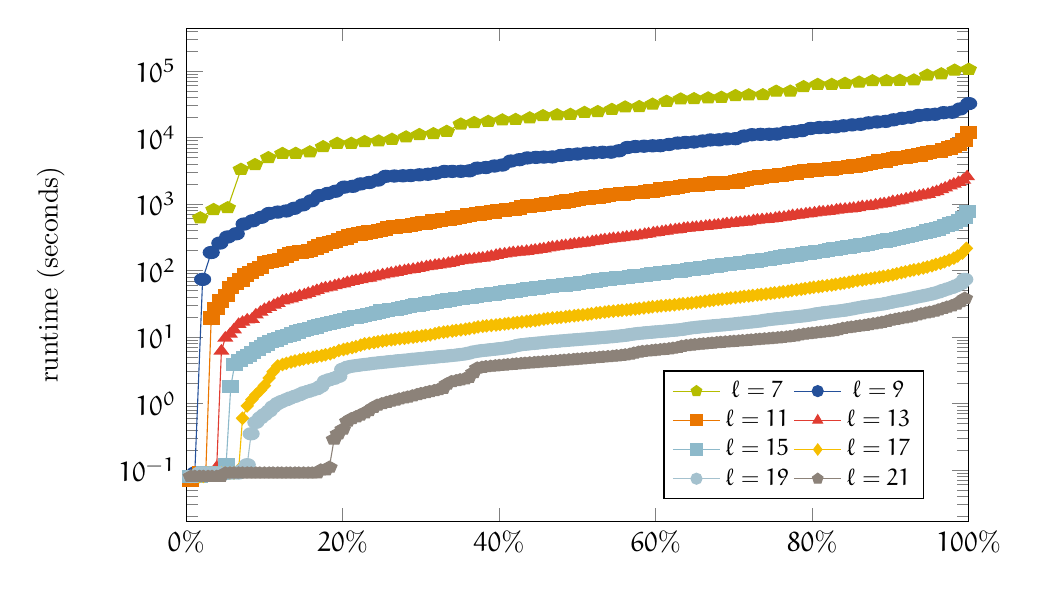
\begin{tikzpicture}
          \begin{axis}[xmin=0,xmax=1, scaled x ticks = false, xticklabel={$\pgfmathprintnumber{\fpeval{\tick*100}}\%$}, legend style={nodes={scale=0.85]}, legend columns=2, at={(0.65,0.3)}}, ymode=log, yscale=1.1, xscale=1.45,ylabel={runtime (seconds)}]


\addplot[color=colh, mark=pentagon*] coordinates
{(0.018, 619.120) (0.035, 825.050) (0.053, 877.390) (0.070, 3317.710) (0.088, 3909.070) (0.105, 4967.080) (0.123, 5743.760) (0.140, 5772.300) (0.158, 6069.700) (0.175, 7264.730) (0.193, 8152.980) (0.211, 8159.750) (0.228, 8673.570) (0.246, 8856.760) (0.263, 9390.630) (0.281, 10183.790) (0.298, 11065.140) (0.316, 11409.190) (0.333, 12353.480) (0.351, 15913.580) (0.368, 16753.970) (0.386, 17439.310) (0.404, 18372.660) (0.421, 18661.440) (0.439, 19718.630) (0.456, 21260.190) (0.474, 21934.550) (0.491, 22253.980) (0.509, 23798.810) (0.526, 24523.990) (0.544, 26414.600) (0.561, 28745.670) (0.579, 29132.260) (0.596, 31687.600) (0.614, 35015.450) (0.632, 37914.080) (0.649, 38318.420) (0.667, 39310.090) (0.684, 40228.570) (0.702, 42643.690) (0.719, 43725.060) (0.737, 43914.580) (0.754, 49597.070) (0.772, 49766.580) (0.789, 58088.050) (0.807, 62723.510) (0.825, 62766.380) (0.842, 65173.950) (0.860, 67982.210) (0.877, 71261.840) (0.895, 71473.600) (0.912, 72403.020) (0.930, 73227.620) (0.947, 86453.640) (0.965, 90611.100) (0.982, 102876.950) (1.000, 105937.760)}; 

\addplot[color=colg, mark=*] coordinates
{(0.011, 0.090) (0.021, 73.430) (0.032, 186.420) (0.043, 258.250) (0.053, 319.150) (0.064, 356.600) (0.074, 499.390) (0.085, 559.150) (0.096, 630.760) (0.106, 720.220) (0.117, 755.080) (0.128, 785.420) (0.138, 860.080) (0.149, 969.300) (0.160, 1116.420) (0.170, 1336.100) (0.181, 1441.650) (0.191, 1555.120) (0.202, 1792.610) (0.213, 1843.780) (0.223, 2004.690) (0.234, 2106.100) (0.245, 2287.180) (0.255, 2604.630) (0.266, 2632.480) (0.277, 2652.070) (0.287, 2679.180) (0.298, 2745.410) (0.309, 2797.420) (0.319, 2898.000) (0.330, 3083.150) (0.340, 3089.300) (0.351, 3100.040) (0.362, 3152.160) (0.372, 3459.860) (0.383, 3534.230) (0.394, 3724.050) (0.404, 3852.280) (0.415, 4425.130) (0.426, 4636.410) (0.436, 4926.570) (0.447, 5018.020) (0.457, 5073.040) (0.468, 5101.420) (0.479, 5373.490) (0.489, 5533.910) (0.500, 5637.890) (0.511, 5809.890) (0.521, 5890.380) (0.532, 5988.060) (0.543, 6014.750) (0.553, 6309.800) (0.564, 7074.490) (0.574, 7302.310) (0.585, 7395.580) (0.596, 7490.720) (0.606, 7532.980) (0.617, 7859.270) (0.628, 8241.560) (0.638, 8429.600) (0.649, 8558.950) (0.660, 8855.170) (0.670, 9186.710) (0.681, 9218.600) (0.691, 9525.930) (0.702, 9598.480) (0.713, 10509.510) (0.723, 11004.970) (0.734, 11139.680) (0.745, 11173.820) (0.755, 11265.450) (0.766, 11933.330) (0.777, 12217.460) (0.787, 12679.550) (0.798, 13672.030) (0.809, 14099.060) (0.819, 14192.870) (0.830, 14469.630) (0.840, 14982.760) (0.851, 15474.030) (0.862, 15799.880) (0.872, 16594.700) (0.883, 17144.330) (0.894, 17473.590) (0.904, 18434.090) (0.915, 19422.090) (0.926, 20143.310) (0.936, 21463.190) (0.947, 22036.630) (0.957, 22336.810) (0.968, 23617.780) (0.979, 23977.920) (0.989, 26857.940) (1.000, 32329.050)};

\addplot[color=colf, mark=square*] coordinates
          {(0.006, 0.070) (0.013, 0.080) (0.019, 0.090) (0.025, 0.090) (0.032, 19.230) (0.038, 26.560) (0.044, 34.860) (0.051, 42.270) (0.057, 55.380) (0.063, 63.960) (0.070, 71.680) (0.076, 85.870) (0.082, 92.740) (0.089, 104.670) (0.095, 110.290) (0.101, 131.000) (0.108, 136.430) (0.114, 140.980) (0.120, 146.800) (0.127, 164.290) (0.133, 176.660) (0.139, 184.390) (0.146, 188.750) (0.152, 191.840) (0.158, 199.480) (0.165, 218.150) (0.171, 233.790) (0.177, 250.400) (0.184, 266.480) (0.190, 272.160) (0.196, 295.880) (0.203, 308.900) (0.209, 329.560) (0.215, 344.760) (0.222, 352.230) (0.228, 365.980) (0.234, 378.710) (0.241, 386.100) (0.247, 395.780) (0.253, 413.430) (0.259, 445.870) (0.266, 451.900) (0.272, 458.310) (0.278, 467.710) (0.285, 476.310) (0.291, 488.920) (0.297, 507.420) (0.304, 515.550) (0.310, 528.530) (0.316, 555.100) (0.323, 565.220) (0.329, 578.210) (0.335, 590.860) (0.342, 616.550) (0.348, 637.600) (0.354, 648.720) (0.361, 683.810) (0.367, 697.710) (0.373, 709.720) (0.380, 728.730) (0.386, 749.140) (0.392, 760.290) (0.399, 794.150) (0.405, 805.180) (0.411, 818.440) (0.418, 824.810) (0.424, 849.200) (0.430, 906.200) (0.437, 928.690) (0.443, 949.190) (0.449, 958.270) (0.456, 981.270) (0.462, 1013.000) (0.468, 1023.630) (0.475, 1048.340) (0.481, 1067.270) (0.487, 1112.920) (0.494, 1127.180) (0.500, 1176.040) (0.506, 1194.780) (0.513, 1228.200) (0.519, 1251.650) (0.525, 1274.630) (0.532, 1286.310) (0.538, 1342.430) (0.544, 1371.620) (0.551, 1405.180) (0.557, 1415.390) (0.563, 1451.600) (0.570, 1472.850) (0.576, 1479.330) (0.582, 1491.490) (0.589, 1525.840) (0.595, 1573.050) (0.601, 1606.920) (0.608, 1679.920) (0.614, 1723.270) (0.620, 1738.110) (0.627, 1785.200) (0.633, 1818.660) (0.639, 1885.900) (0.646, 1909.530) (0.652, 1921.190) (0.658, 1945.820) (0.665, 1976.490) (0.671, 2025.640) (0.677, 2062.040) (0.684, 2073.200) (0.690, 2087.250) (0.696, 2124.670) (0.703, 2142.100) (0.709, 2260.750) (0.715, 2331.620) (0.722, 2442.020) (0.728, 2467.840) (0.734, 2549.780) (0.741, 2597.900) (0.747, 2634.110) (0.753, 2672.820) (0.759, 2723.050) (0.766, 2791.230) (0.772, 2856.470) (0.778, 2931.100) (0.785, 3043.270) (0.791, 3133.510) (0.797, 3213.070) (0.804, 3250.630) (0.810, 3311.980) (0.816, 3331.460) (0.823, 3355.840) (0.829, 3423.040) (0.835, 3496.220) (0.842, 3550.510) (0.848, 3631.280) (0.854, 3736.040) (0.861, 3816.090) (0.867, 3924.990) (0.873, 4026.930) (0.880, 4244.580) (0.886, 4415.720) (0.892, 4450.490) (0.899, 4654.480) (0.905, 4804.600) (0.911, 4957.280) (0.918, 5060.730) (0.924, 5138.860) (0.930, 5296.860) (0.937, 5454.170) (0.943, 5735.770) (0.949, 5949.900) (0.956, 6105.470) (0.962, 6219.490) (0.968, 6545.830) (0.975, 6940.710) (0.981, 7369.190) (0.987, 7887.620) (0.994, 9146.710) (1.000, 11844.050)};
          
                    \addplot[color=cola, mark=triangle*] coordinates {(0.006, 0.080) (0.011, 0.080) (0.017, 0.080) (0.022, 0.090) (0.028, 0.090) (0.033, 0.090) (0.039, 0.110) (0.045, 6.170) (0.050, 9.670) (0.056, 11.030) (0.061, 12.870) (0.067, 15.530) (0.072, 16.710) (0.078, 18.110) (0.084, 18.510) (0.089, 21.560) (0.095, 23.770) (0.100, 26.060) (0.106, 28.010) (0.112, 30.160) (0.117, 32.090) (0.123, 34.960) (0.128, 36.130) (0.134, 37.560) (0.139, 39.400) (0.145, 41.820) (0.151, 43.280) (0.156, 45.470) (0.162, 47.760) (0.167, 50.280) (0.173, 53.160) (0.178, 55.020) (0.184, 56.620) (0.190, 59.260) (0.195, 61.350) (0.201, 63.070) (0.206, 66.330) (0.212, 68.790) (0.217, 70.960) (0.223, 73.300) (0.229, 75.790) (0.234, 77.170) (0.240, 80.360) (0.245, 82.980) (0.251, 86.530) (0.257, 88.820) (0.262, 91.680) (0.268, 94.260) (0.273, 97.500) (0.279, 99.520) (0.284, 102.120) (0.290, 104.430) (0.296, 107.480) (0.301, 111.170) (0.307, 114.270) (0.312, 116.880) (0.318, 120.090) (0.323, 121.910) (0.329, 124.890) (0.335, 128.750) (0.340, 131.510) (0.346, 136.950) (0.351, 141.060) (0.357, 144.210) (0.362, 146.680) (0.368, 149.140) (0.374, 152.660) (0.379, 154.470) (0.385, 158.670) (0.390, 163.630) (0.396, 169.940) (0.401, 174.910) (0.407, 177.790) (0.413, 182.330) (0.418, 186.470) (0.424, 188.920) (0.429, 191.480) (0.435, 194.990) (0.441, 199.130) (0.446, 203.130) (0.452, 208.480) (0.457, 212.200) (0.463, 219.020) (0.468, 224.880) (0.474, 229.520) (0.480, 235.360) (0.485, 238.400) (0.491, 245.040) (0.496, 250.170) (0.502, 255.070) (0.507, 258.820) (0.513, 264.050) (0.519, 272.110) (0.524, 277.760) (0.530, 285.420) (0.535, 291.320) (0.541, 296.040) (0.546, 303.230) (0.552, 307.510) (0.558, 312.410) (0.563, 319.920) (0.569, 324.260) (0.574, 332.720) (0.580, 340.510) (0.586, 350.850) (0.591, 357.050) (0.597, 369.160) (0.602, 374.720) (0.608, 383.840) (0.613, 391.480) (0.619, 404.260) (0.625, 410.740) (0.630, 418.130) (0.636, 430.530) (0.641, 435.360) (0.647, 441.470) (0.652, 447.180) (0.658, 456.790) (0.664, 463.500) (0.669, 472.080) (0.675, 478.040) (0.680, 485.090) (0.686, 494.670) (0.691, 507.430) (0.697, 512.680) (0.703, 522.190) (0.708, 530.290) (0.714, 537.140) (0.719, 545.320) (0.725, 562.580) (0.730, 573.440) (0.736, 582.470) (0.742, 589.900) (0.747, 596.650) (0.753, 611.160) (0.758, 626.430) (0.764, 635.710) (0.770, 653.060) (0.775, 672.320) (0.781, 682.950) (0.786, 695.250) (0.792, 711.750) (0.797, 720.290) (0.803, 735.410) (0.809, 756.610) (0.814, 762.320) (0.820, 775.290) (0.825, 789.300) (0.831, 813.440) (0.836, 826.880) (0.842, 838.540) (0.848, 850.590) (0.853, 864.700) (0.859, 885.200) (0.864, 913.120) (0.870, 921.570) (0.875, 938.960) (0.881, 970.040) (0.887, 994.120) (0.892, 1014.060) (0.898, 1041.930) (0.903, 1091.910) (0.909, 1112.920) (0.914, 1148.580) (0.920, 1196.780) (0.926, 1237.560) (0.931, 1277.160) (0.937, 1324.070) (0.942, 1365.430) (0.948, 1405.300) (0.954, 1486.810) (0.959, 1542.070) (0.965, 1651.450) (0.970, 1746.740) (0.976, 1877.550) (0.981, 1993.450) (0.987, 2120.810) (0.993, 2293.800) (0.998, 2578.610)};


          \addplot[color=colb, mark=square*] coordinates {(0.006, 0.080) (0.011, 0.080) (0.017, 0.080) (0.023, 0.090) (0.028, 0.090) (0.034, 0.090) (0.040, 0.090) (0.045, 0.090) (0.051, 0.120) (0.057, 1.810) (0.062, 3.840) (0.068, 4.450) (0.074, 4.860) (0.080, 5.280) (0.085, 5.780) (0.091, 6.570) (0.097, 7.180) (0.102, 7.860) (0.108, 8.520) (0.114, 9.030) (0.119, 9.470) (0.125, 10.070) (0.131, 10.540) (0.136, 11.060) (0.142, 11.930) (0.148, 12.460) (0.153, 13.030) (0.159, 13.460) (0.165, 14.090) (0.170, 14.820) (0.176, 15.430) (0.182, 15.990) (0.187, 16.530) (0.193, 17.190) (0.199, 17.850) (0.204, 18.500) (0.210, 19.420) (0.216, 20.010) (0.221, 20.530) (0.227, 21.160) (0.233, 21.810) (0.239, 22.590) (0.244, 23.540) (0.250, 24.600) (0.256, 25.140) (0.261, 25.660) (0.267, 26.190) (0.273, 26.840) (0.278, 27.700) (0.284, 28.610) (0.290, 29.440) (0.295, 30.260) (0.301, 30.920) (0.307, 31.810) (0.312, 32.380) (0.318, 33.140) (0.324, 33.960) (0.329, 34.830) (0.335, 35.940) (0.341, 36.760) (0.346, 37.490) (0.352, 38.300) (0.358, 38.930) (0.363, 39.930) (0.369, 40.880) (0.375, 41.570) (0.380, 42.660) (0.386, 43.370) (0.392, 44.410) (0.398, 45.460) (0.403, 46.470) (0.409, 47.330) (0.415, 48.090) (0.420, 48.980) (0.426, 50.430) (0.432, 51.770) (0.437, 52.540) (0.443, 53.300) (0.449, 54.540) (0.454, 56.060) (0.460, 56.870) (0.466, 57.920) (0.471, 58.770) (0.477, 59.670) (0.483, 60.600) (0.488, 61.780) (0.494, 62.920) (0.500, 63.990) (0.505, 65.190) (0.511, 66.580) (0.517, 68.020) (0.522, 69.700) (0.528, 71.600) (0.534, 73.090) (0.539, 74.180) (0.545, 75.880) (0.551, 76.900) (0.557, 78.190) (0.562, 79.360) (0.568, 80.440) (0.574, 82.290) (0.579, 83.800) (0.585, 85.000) (0.591, 86.540) (0.596, 88.140) (0.602, 89.880) (0.608, 91.940) (0.613, 93.750) (0.619, 95.340) (0.625, 96.990) (0.630, 98.530) (0.636, 100.620) (0.642, 102.800) (0.647, 105.140) (0.653, 107.220) (0.659, 109.260) (0.664, 111.380) (0.670, 113.910) (0.676, 116.630) (0.681, 119.090) (0.687, 121.600) (0.693, 123.820) (0.698, 126.010) (0.704, 128.440) (0.710, 131.080) (0.716, 133.200) (0.721, 135.930) (0.727, 139.240) (0.733, 142.140) (0.738, 144.940) (0.744, 147.950) (0.750, 151.940) (0.755, 156.070) (0.761, 159.880) (0.767, 164.360) (0.772, 167.460) (0.778, 170.900) (0.784, 175.000) (0.789, 179.270) (0.795, 183.080) (0.801, 186.540) (0.806, 190.630) (0.812, 195.320) (0.818, 198.900) (0.823, 204.810) (0.829, 210.550) (0.835, 215.060) (0.840, 219.220) (0.846, 224.470) (0.852, 229.510) (0.857, 235.140) (0.863, 241.940) (0.869, 247.660) (0.875, 254.780) (0.880, 261.720) (0.886, 271.480) (0.892, 278.060) (0.897, 286.250) (0.903, 294.710) (0.909, 305.670) (0.914, 313.860) (0.920, 324.860) (0.926, 335.480) (0.931, 348.180) (0.937, 361.670) (0.943, 376.800) (0.948, 393.290) (0.954, 406.130) (0.960, 422.120) (0.965, 444.460) (0.971, 471.710) (0.977, 498.060) (0.982, 528.860) (0.988, 571.220) (0.994, 625.030) (0.999, 772.190)};
          
                  
          \addplot[color=colc, mark=diamond*] coordinates {(0.006, 0.080) (0.011, 0.080) (0.017, 0.080) (0.022, 0.080) (0.028, 0.090) (0.033, 0.090) (0.039, 0.090) (0.045, 0.090) (0.050, 0.090) (0.056, 0.090) (0.061, 0.090) (0.067, 0.100) (0.072, 0.600) (0.078, 0.920) (0.084, 1.150) (0.089, 1.350) (0.095, 1.590) (0.100, 1.860) (0.106, 2.420) (0.111, 3.000) (0.117, 3.660) (0.123, 3.860) (0.128, 4.020) (0.134, 4.200) (0.139, 4.350) (0.145, 4.510) (0.150, 4.660) (0.156, 4.800) (0.162, 4.950) (0.167, 5.100) (0.173, 5.240) (0.178, 5.400) (0.184, 5.590) (0.189, 5.850) (0.195, 6.240) (0.201, 6.490) (0.206, 6.680) (0.212, 6.920) (0.217, 7.160) (0.223, 7.530) (0.228, 7.870) (0.234, 8.060) (0.240, 8.260) (0.245, 8.480) (0.251, 8.700) (0.256, 8.890) (0.262, 9.060) (0.267, 9.240) (0.273, 9.420) (0.279, 9.590) (0.284, 9.790) (0.290, 9.970) (0.295, 10.160) (0.301, 10.340) (0.306, 10.560) (0.312, 10.780) (0.318, 11.180) (0.323, 11.570) (0.329, 11.840) (0.334, 12.050) (0.340, 12.310) (0.345, 12.540) (0.351, 12.800) (0.357, 13.070) (0.362, 13.370) (0.368, 13.750) (0.373, 14.160) (0.379, 14.440) (0.384, 14.720) (0.390, 14.930) (0.396, 15.170) (0.401, 15.420) (0.407, 15.690) (0.412, 15.950) (0.418, 16.210) (0.423, 16.500) (0.429, 16.850) (0.435, 17.130) (0.440, 17.430) (0.446, 17.710) (0.451, 18.090) (0.457, 18.570) (0.462, 18.990) (0.468, 19.290) (0.474, 19.580) (0.479, 19.870) (0.485, 20.160) (0.490, 20.510) (0.496, 20.850) (0.501, 21.170) (0.507, 21.520) (0.513, 21.910) (0.518, 22.400) (0.524, 22.920) (0.529, 23.300) (0.535, 23.700) (0.540, 24.110) (0.546, 24.470) (0.552, 24.830) (0.557, 25.180) (0.563, 25.550) (0.568, 25.900) (0.574, 26.360) (0.579, 26.830) (0.585, 27.340) (0.591, 27.930) (0.596, 28.420) (0.602, 28.850) (0.607, 29.300) (0.613, 29.720) (0.618, 30.110) (0.624, 30.570) (0.630, 31.090) (0.635, 31.560) (0.641, 32.000) (0.646, 32.490) (0.652, 33.080) (0.657, 33.710) (0.663, 34.560) (0.669, 35.260) (0.674, 35.860) (0.680, 36.540) (0.685, 37.140) (0.691, 37.770) (0.696, 38.550) (0.702, 39.350) (0.708, 40.000) (0.713, 40.690) (0.719, 41.400) (0.724, 42.120) (0.730, 42.830) (0.735, 43.590) (0.741, 44.360) (0.747, 45.240) (0.752, 46.090) (0.758, 46.940) (0.763, 47.760) (0.769, 48.780) (0.774, 50.050) (0.780, 51.100) (0.786, 52.230) (0.791, 53.360) (0.797, 54.660) (0.802, 55.740) (0.808, 56.930) (0.813, 58.080) (0.819, 59.270) (0.825, 60.480) (0.830, 61.860) (0.836, 63.270) (0.841, 64.790) (0.847, 66.400) (0.852, 68.630) (0.858, 70.550) (0.864, 72.100) (0.869, 73.820) (0.875, 75.580) (0.880, 77.460) (0.886, 79.470) (0.891, 81.370) (0.897, 83.690) (0.903, 86.390) (0.908, 89.380) (0.914, 92.700) (0.919, 95.410) (0.925, 98.920) (0.930, 101.920) (0.936, 104.700) (0.942, 108.810) (0.947, 113.000) (0.953, 117.760) (0.958, 123.720) (0.964, 128.660) (0.969, 135.210) (0.975, 143.440) (0.981, 153.050) (0.986, 165.580) (0.992, 182.640) (0.997, 214.970)};
          




  \addplot[color=cold, mark=*] coordinates {(0.006, 0.080) (0.011, 0.080) (0.017, 0.090) (0.022, 0.090) (0.028, 0.090) (0.033, 0.090) (0.039, 0.090) (0.044, 0.090) (0.050, 0.090) (0.056, 0.090) (0.061, 0.090) (0.067, 0.090) (0.072, 0.100) (0.078, 0.120) (0.083, 0.350) (0.089, 0.520) (0.095, 0.610) (0.100, 0.680) (0.106, 0.770) (0.111, 0.890) (0.117, 1.000) (0.122, 1.070) (0.128, 1.140) (0.133, 1.210) (0.139, 1.280) (0.145, 1.360) (0.150, 1.450) (0.156, 1.520) (0.161, 1.590) (0.167, 1.670) (0.172, 1.810) (0.178, 2.170) (0.183, 2.280) (0.189, 2.390) (0.195, 2.560) (0.200, 3.270) (0.206, 3.510) (0.211, 3.620) (0.217, 3.710) (0.222, 3.780) (0.228, 3.860) (0.234, 3.930) (0.239, 4.010) (0.245, 4.080) (0.250, 4.140) (0.256, 4.210) (0.261, 4.270) (0.267, 4.340) (0.272, 4.410) (0.278, 4.470) (0.284, 4.540) (0.289, 4.620) (0.295, 4.680) (0.300, 4.750) (0.306, 4.820) (0.311, 4.890) (0.317, 4.960) (0.322, 5.030) (0.328, 5.100) (0.334, 5.180) (0.339, 5.260) (0.345, 5.340) (0.350, 5.440) (0.356, 5.550) (0.361, 5.710) (0.367, 5.960) (0.373, 6.120) (0.378, 6.240) (0.384, 6.340) (0.389, 6.450) (0.395, 6.550) (0.400, 6.670) (0.406, 6.790) (0.411, 6.940) (0.417, 7.140) (0.423, 7.450) (0.428, 7.640) (0.434, 7.770) (0.439, 7.890) (0.445, 8.000) (0.450, 8.120) (0.456, 8.240) (0.461, 8.370) (0.467, 8.490) (0.473, 8.600) (0.478, 8.710) (0.484, 8.820) (0.489, 8.930) (0.495, 9.040) (0.500, 9.140) (0.506, 9.260) (0.512, 9.370) (0.517, 9.490) (0.523, 9.610) (0.528, 9.720) (0.534, 9.840) (0.539, 9.960) (0.545, 10.100) (0.550, 10.240) (0.556, 10.410) (0.562, 10.600) (0.567, 10.860) (0.573, 11.110) (0.578, 11.300) (0.584, 11.470) (0.589, 11.630) (0.595, 11.790) (0.600, 11.940) (0.606, 12.090) (0.612, 12.250) (0.617, 12.420) (0.623, 12.590) (0.628, 12.770) (0.634, 12.990) (0.639, 13.310) (0.645, 13.650) (0.651, 13.900) (0.656, 14.120) (0.662, 14.320) (0.667, 14.530) (0.673, 14.720) (0.678, 14.890) (0.684, 15.100) (0.689, 15.310) (0.695, 15.520) (0.701, 15.770) (0.706, 16.040) (0.712, 16.290) (0.717, 16.540) (0.723, 16.810) (0.728, 17.070) (0.734, 17.380) (0.739, 17.810) (0.745, 18.250) (0.751, 18.570) (0.756, 18.870) (0.762, 19.160) (0.767, 19.470) (0.773, 19.760) (0.778, 20.090) (0.784, 20.410) (0.790, 20.770) (0.795, 21.170) (0.801, 21.720) (0.806, 22.380) (0.812, 22.870) (0.817, 23.330) (0.823, 23.760) (0.828, 24.190) (0.834, 24.620) (0.840, 25.110) (0.845, 25.700) (0.851, 26.390) (0.856, 27.170) (0.862, 27.950) (0.867, 28.640) (0.873, 29.230) (0.878, 29.880) (0.884, 30.580) (0.890, 31.240) (0.895, 32.070) (0.901, 33.220) (0.906, 34.270) (0.912, 35.150) (0.917, 36.150) (0.923, 37.300) (0.929, 38.690) (0.934, 39.920) (0.940, 41.160) (0.945, 42.350) (0.951, 43.830) (0.956, 45.410) (0.962, 47.540) (0.967, 50.040) (0.973, 52.770) (0.979, 55.630) (0.984, 58.810) (0.990, 63.550) (0.995, 73.420)};

          \addplot[color=cole, mark=pentagon*] coordinates {(0.006, 0.080) (0.011, 0.080) (0.017, 0.080) (0.022, 0.080) (0.028, 0.080) (0.033, 0.080) (0.039, 0.080) (0.044, 0.080) (0.050, 0.090) (0.056, 0.090) (0.061, 0.090) (0.067, 0.090) (0.072, 0.090) (0.078, 0.090) (0.083, 0.090) (0.089, 0.090) (0.094, 0.090) (0.100, 0.090) (0.106, 0.090) (0.111, 0.090) (0.117, 0.090) (0.122, 0.090) (0.128, 0.090) (0.133, 0.090) (0.139, 0.090) (0.144, 0.090) (0.150, 0.090) (0.156, 0.090) (0.161, 0.090) (0.167, 0.090) (0.172, 0.100) (0.178, 0.100) (0.183, 0.110) (0.189, 0.290) (0.194, 0.350) (0.200, 0.410) (0.206, 0.540) (0.211, 0.590) (0.217, 0.630) (0.222, 0.670) (0.228, 0.720) (0.233, 0.780) (0.239, 0.870) (0.244, 0.940) (0.250, 0.990) (0.256, 1.040) (0.261, 1.080) (0.267, 1.120) (0.272, 1.170) (0.278, 1.210) (0.283, 1.250) (0.289, 1.300) (0.295, 1.360) (0.300, 1.410) (0.306, 1.460) (0.311, 1.510) (0.317, 1.560) (0.322, 1.610) (0.328, 1.680) (0.333, 1.960) (0.339, 2.130) (0.345, 2.200) (0.350, 2.270) (0.356, 2.350) (0.361, 2.470) (0.367, 2.920) (0.372, 3.410) (0.378, 3.500) (0.383, 3.570) (0.389, 3.630) (0.395, 3.680) (0.400, 3.730) (0.406, 3.780) (0.411, 3.830) (0.417, 3.880) (0.422, 3.930) (0.428, 3.980) (0.433, 4.030) (0.439, 4.080) (0.445, 4.120) (0.450, 4.170) (0.456, 4.220) (0.461, 4.260) (0.467, 4.310) (0.472, 4.360) (0.478, 4.420) (0.483, 4.470) (0.489, 4.530) (0.495, 4.580) (0.500, 4.640) (0.506, 4.690) (0.511, 4.750) (0.517, 4.810) (0.522, 4.870) (0.528, 4.930) (0.533, 5.000) (0.539, 5.060) (0.545, 5.130) (0.550, 5.210) (0.556, 5.290) (0.561, 5.380) (0.567, 5.510) (0.572, 5.720) (0.578, 5.920) (0.583, 6.050) (0.589, 6.150) (0.595, 6.240) (0.600, 6.340) (0.606, 6.430) (0.611, 6.530) (0.617, 6.640) (0.622, 6.770) (0.628, 6.950) (0.633, 7.240) (0.639, 7.420) (0.645, 7.550) (0.650, 7.660) (0.656, 7.770) (0.661, 7.870) (0.667, 7.980) (0.672, 8.090) (0.678, 8.210) (0.683, 8.310) (0.689, 8.410) (0.695, 8.510) (0.700, 8.600) (0.706, 8.700) (0.711, 8.800) (0.717, 8.900) (0.722, 9.010) (0.728, 9.130) (0.733, 9.240) (0.739, 9.360) (0.745, 9.470) (0.750, 9.590) (0.756, 9.720) (0.761, 9.850) (0.767, 9.990) (0.772, 10.160) (0.778, 10.400) (0.783, 10.720) (0.789, 10.990) (0.795, 11.200) (0.800, 11.400) (0.806, 11.590) (0.811, 11.790) (0.817, 12.000) (0.822, 12.240) (0.828, 12.500) (0.833, 12.920) (0.839, 13.450) (0.845, 13.780) (0.850, 14.080) (0.856, 14.370) (0.861, 14.680) (0.867, 14.990) (0.872, 15.340) (0.878, 15.770) (0.884, 16.170) (0.889, 16.600) (0.895, 17.210) (0.900, 17.900) (0.906, 18.400) (0.911, 18.880) (0.917, 19.380) (0.922, 19.950) (0.928, 20.580) (0.934, 21.550) (0.939, 22.280) (0.945, 22.930) (0.950, 23.620) (0.956, 24.390) (0.961, 25.480) (0.967, 26.840) (0.972, 28.080) (0.978, 29.410) (0.984, 31.150) (0.989, 33.970) (0.995, 38.170)};

          
\legend{{$\ell=7$},{$\ell=9$},{$\ell=11$},{$\ell=13$},{$\ell=15$},{$\ell=17$},{$\ell=19$},{$\ell=21$}}
          
          \end{axis}
\end{tikzpicture}



	
}

\newtheorem{conjecture}[theorem]{\translate{Conjecture}}

\frame{
	\frametitle{Empty Hexagon Theorem Summary}
	
\large

\bigskip


\structure{Theorem}:  $h(6) = 30$
%Solving the only remaining hole problem is within reach
\begin{itemize}
\item Partitioned problem using 312\,418 cubes $(\ell = 21)$
%\item Hardest subproblem: 5\,457 seconds
\item Total runtime: 17\,000 CPU hours on AWS
\item Linear speedups using 1\,000 machines
\item Proof: 180 terabytes in unprocessed LRAT format
\item Validated with formally-verified checker
%\item Strong evidence that the conjecture holds
%\item An initial run without proof construction finished
%\item The heuristics for smaller problems are also effective
%\item Rough estimation: 100,000 CPU hours solving + checking
%\item Linear-time scaling with thousands of cores
\end{itemize}

\bigskip

\parindent -15pt


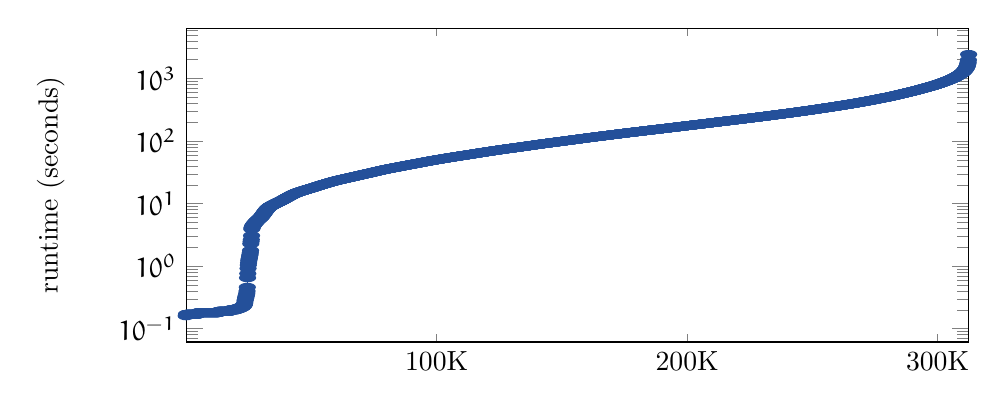
\begin{tikzpicture}
          \begin{axis}[xmin=1,xmax=312418, xtick={100000,200000,300000}, xticklabels={100K, 200K,300K}, scaled x ticks = false,ymode=log, yscale=0.7, xscale=1.45,ylabel={runtime (seconds)}]
          \addplot[color=colg, mark=*] coordinates {(1, 0.160) (101, 0.170) (201, 0.170) (301, 0.170) (401, 0.170) (501, 0.170) (601, 0.170) (701, 0.170) (801, 0.170) (901, 0.170) (1001, 0.170) (1101, 0.170) (1201, 0.170) (1301, 0.170) (1401, 0.170) (1501, 0.170) (1601, 0.170) (1701, 0.170) (1801, 0.170) (1901, 0.170) (2001, 0.170) (2101, 0.170) (2201, 0.170) (2301, 0.170) (2401, 0.170) (2501, 0.170) (2601, 0.170) (2701, 0.170) (2801, 0.170) (2901, 0.170) (3001, 0.170) (3101, 0.170) (3201, 0.170) (3301, 0.170) (3401, 0.170) (3501, 0.170) (3601, 0.170) (3701, 0.170) (3801, 0.170) (3901, 0.170) (4001, 0.170) (4101, 0.170) (4201, 0.170) (4301, 0.170) (4401, 0.170) (4501, 0.170) (4601, 0.170) (4701, 0.180) (4801, 0.180) (4901, 0.180) (5001, 0.180) (5101, 0.180) (5201, 0.180) (5301, 0.180) (5401, 0.180) (5501, 0.180) (5601, 0.180) (5701, 0.180) (5801, 0.180) (5901, 0.180) (6001, 0.180) (6101, 0.180) (6201, 0.180) (6301, 0.180) (6401, 0.180) (6501, 0.180) (6601, 0.180) (6701, 0.180) (6801, 0.180) (6901, 0.180) (7001, 0.180) (7101, 0.180) (7201, 0.180) (7301, 0.180) (7401, 0.180) (7501, 0.180) (7601, 0.180) (7701, 0.180) (7801, 0.180) (7901, 0.180) (8001, 0.180) (8101, 0.180) (8201, 0.180) (8301, 0.180) (8401, 0.180) (8501, 0.180) (8601, 0.180) (8701, 0.180) (8801, 0.180) (8901, 0.180) (9001, 0.180) (9101, 0.180) (9201, 0.180) (9301, 0.180) (9401, 0.180) (9501, 0.180) (9601, 0.180) (9701, 0.180) (9801, 0.180) (9901, 0.180) (10001, 0.180) (10101, 0.180) (10201, 0.180) (10301, 0.180) (10401, 0.180) (10501, 0.180) (10601, 0.180) (10701, 0.180) (10801, 0.180) (10901, 0.180) (11001, 0.180) (11101, 0.180) (11201, 0.180) (11301, 0.180) (11401, 0.180) (11501, 0.180) (11601, 0.180) (11701, 0.180) (11801, 0.180) (11901, 0.180) (12001, 0.180) (12101, 0.180) (12201, 0.180) (12301, 0.180) (12401, 0.180) (12501, 0.180) (12601, 0.180) (12701, 0.180) (12801, 0.180) (12901, 0.180) (13001, 0.190) (13101, 0.190) (13201, 0.190) (13301, 0.190) (13401, 0.190) (13501, 0.190) (13601, 0.190) (13701, 0.190) (13801, 0.190) (13901, 0.190) (14001, 0.190) (14101, 0.190) (14201, 0.190) (14301, 0.190) (14401, 0.190) (14501, 0.190) (14601, 0.190) (14701, 0.190) (14801, 0.190) (14901, 0.190) (15001, 0.190) (15101, 0.190) (15201, 0.190) (15301, 0.190) (15401, 0.190) (15501, 0.190) (15601, 0.190) (15701, 0.190) (15801, 0.190) (15901, 0.190) (16001, 0.190) (16101, 0.190) (16201, 0.190) (16301, 0.190) (16401, 0.190) (16501, 0.190) (16601, 0.190) (16701, 0.190) (16801, 0.190) (16901, 0.190) (17001, 0.190) (17101, 0.190) (17201, 0.190) (17301, 0.190) (17401, 0.190) (17501, 0.190) (17601, 0.200) (17701, 0.200) (17801, 0.200) (17901, 0.200) (18001, 0.200) (18101, 0.200) (18201, 0.200) (18301, 0.200) (18401, 0.200) (18501, 0.200) (18601, 0.200) (18701, 0.200) (18801, 0.200) (18901, 0.200) (19001, 0.200) (19101, 0.200) (19201, 0.200) (19301, 0.200) (19401, 0.200) (19501, 0.200) (19601, 0.200) (19701, 0.200) (19801, 0.200) (19901, 0.200) (20001, 0.200) (20101, 0.210) (20201, 0.210) (20301, 0.210) (20401, 0.210) (20501, 0.210) (20601, 0.210) (20701, 0.210) (20801, 0.210) (20901, 0.210) (21001, 0.210) (21101, 0.210) (21201, 0.210) (21301, 0.210) (21401, 0.210) (21501, 0.210) (21601, 0.220) (21701, 0.220) (21801, 0.220) (21901, 0.220) (22001, 0.220) (22101, 0.220) (22201, 0.220) (22301, 0.220) (22401, 0.220) (22501, 0.230) (22601, 0.230) (22701, 0.230) (22801, 0.230) (22901, 0.230) (23001, 0.240) (23101, 0.240) (23201, 0.240) (23301, 0.250) (23401, 0.260) (23501, 0.280) (23601, 0.290) (23701, 0.310) (23801, 0.310) (23901, 0.330) (24001, 0.340) (24101, 0.350) (24201, 0.370) (24301, 0.400) (24401, 0.460) (24501, 0.650) (24601, 0.760) (24701, 0.920) (24801, 1.040) (24901, 1.130) (25001, 1.220) (25101, 1.290) (25201, 1.340) (25301, 1.400) (25401, 1.480) (25501, 1.550) (25601, 1.640) (25701, 1.780) (25801, 2.280) (25901, 2.470) (26001, 2.650) (26101, 3.070) (26201, 3.920) (26301, 4.090) (26401, 4.220) (26501, 4.300) (26601, 4.380) (26701, 4.450) (26801, 4.520) (26901, 4.570) (27001, 4.630) (27101, 4.690) (27201, 4.740) (27301, 4.800) (27401, 4.850) (27501, 4.900) (27601, 4.950) (27701, 5.000) (27801, 5.050) (27901, 5.110) (28001, 5.160) (28101, 5.210) (28201, 5.260) (28301, 5.310) (28401, 5.360) (28501, 5.410) (28601, 5.450) (28701, 5.500) (28801, 5.540) (28901, 5.590) (29001, 5.630) (29101, 5.690) (29201, 5.740) (29301, 5.780) (29401, 5.830) (29501, 5.880) (29601, 5.930) (29701, 5.980) (29801, 6.050) (29901, 6.100) (30001, 6.160) (30101, 6.230) (30201, 6.320) (30301, 6.390) (30401, 6.450) (30501, 6.540) (30601, 6.630) (30701, 6.710) (30801, 6.800) (30901, 6.880) (31001, 6.970) (31101, 7.050) (31201, 7.150) (31301, 7.240) (31401, 7.350) (31501, 7.430) (31601, 7.530) (31701, 7.620) (31801, 7.710) (31901, 7.800) (32001, 7.900) (32101, 7.990) (32201, 8.080) (32301, 8.160) (32401, 8.250) (32501, 8.320) (32601, 8.410) (32701, 8.480) (32801, 8.540) (32901, 8.600) (33001, 8.670) (33101, 8.730) (33201, 8.790) (33301, 8.860) (33401, 8.920) (33501, 8.970) (33601, 9.030) (33701, 9.090) (33801, 9.140) (33901, 9.180) (34001, 9.230) (34101, 9.280) (34201, 9.330) (34301, 9.380) (34401, 9.420) (34501, 9.470) (34601, 9.510) (34701, 9.560) (34801, 9.600) (34901, 9.650) (35001, 9.690) (35101, 9.730) (35201, 9.780) (35301, 9.820) (35401, 9.870) (35501, 9.930) (35601, 9.980) (35701, 10.020) (35801, 10.070) (35901, 10.120) (36001, 10.170) (36101, 10.220) (36201, 10.270) (36301, 10.310) (36401, 10.360) (36501, 10.400) (36601, 10.430) (36701, 10.490) (36801, 10.530) (36901, 10.580) (37001, 10.620) (37101, 10.670) (37201, 10.710) (37301, 10.760) (37401, 10.800) (37501, 10.850) (37601, 10.910) (37701, 10.960) (37801, 11.010) (37901, 11.070) (38001, 11.120) (38101, 11.170) (38201, 11.220) (38301, 11.270) (38401, 11.330) (38501, 11.380) (38601, 11.440) (38701, 11.500) (38801, 11.560) (38901, 11.620) (39001, 11.680) (39101, 11.730) (39201, 11.790) (39301, 11.860) (39401, 11.930) (39501, 11.990) (39601, 12.060) (39701, 12.130) (39801, 12.190) (39901, 12.250) (40001, 12.310) (40101, 12.370) (40201, 12.430) (40301, 12.490) (40401, 12.560) (40501, 12.620) (40601, 12.680) (40701, 12.750) (40801, 12.820) (40901, 12.880) (41001, 12.940) (41101, 13.000) (41201, 13.060) (41301, 13.120) (41401, 13.200) (41501, 13.270) (41601, 13.340) (41701, 13.420) (41801, 13.480) (41901, 13.550) (42001, 13.620) (42101, 13.680) (42201, 13.740) (42301, 13.810) (42401, 13.860) (42501, 13.920) (42601, 13.990) (42701, 14.050) (42801, 14.120) (42901, 14.190) (43001, 14.240) (43101, 14.310) (43201, 14.350) (43301, 14.410) (43401, 14.470) (43501, 14.520) (43601, 14.580) (43701, 14.640) (43801, 14.700) (43901, 14.760) (44001, 14.810) (44101, 14.860) (44201, 14.910) (44301, 14.960) (44401, 15.010) (44501, 15.070) (44601, 15.120) (44701, 15.170) (44801, 15.220) (44901, 15.270) (45001, 15.330) (45101, 15.380) (45201, 15.410) (45301, 15.470) (45401, 15.520) (45501, 15.560) (45601, 15.610) (45701, 15.660) (45801, 15.710) (45901, 15.750) (46001, 15.800) (46101, 15.850) (46201, 15.900) (46301, 15.950) (46401, 15.980) (46501, 16.030) (46601, 16.080) (46701, 16.120) (46801, 16.170) (46901, 16.220) (47001, 16.270) (47101, 16.310) (47201, 16.350) (47301, 16.400) (47401, 16.440) (47501, 16.490) (47601, 16.540) (47701, 16.590) (47801, 16.640) (47901, 16.690) (48001, 16.740) (48101, 16.790) (48201, 16.830) (48301, 16.880) (48401, 16.920) (48501, 16.980) (48601, 17.010) (48701, 17.060) (48801, 17.110) (48901, 17.160) (49001, 17.210) (49101, 17.250) (49201, 17.300) (49301, 17.350) (49401, 17.420) (49501, 17.460) (49601, 17.500) (49701, 17.550) (49801, 17.600) (49901, 17.640) (50001, 17.700) (50101, 17.740) (50201, 17.790) (50301, 17.850) (50401, 17.890) (50501, 17.940) (50601, 17.990) (50701, 18.050) (50801, 18.100) (50901, 18.150) (51001, 18.200) (51101, 18.260) (51201, 18.320) (51301, 18.370) (51401, 18.430) (51501, 18.480) (51601, 18.530) (51701, 18.600) (51801, 18.650) (51901, 18.710) (52001, 18.770) (52101, 18.830) (52201, 18.880) (52301, 18.950) (52401, 19.000) (52501, 19.040) (52601, 19.110) (52701, 19.170) (52801, 19.220) (52901, 19.280) (53001, 19.330) (53101, 19.380) (53201, 19.450) (53301, 19.500) (53401, 19.560) (53501, 19.610) (53601, 19.670) (53701, 19.730) (53801, 19.800) (53901, 19.850) (54001, 19.910) (54101, 19.970) (54201, 20.030) (54301, 20.080) (54401, 20.140) (54501, 20.190) (54601, 20.250) (54701, 20.300) (54801, 20.360) (54901, 20.410) (55001, 20.450) (55101, 20.510) (55201, 20.560) (55301, 20.620) (55401, 20.670) (55501, 20.750) (55601, 20.810) (55701, 20.870) (55801, 20.920) (55901, 20.990) (56001, 21.040) (56101, 21.090) (56201, 21.160) (56301, 21.200) (56401, 21.260) (56501, 21.320) (56601, 21.390) (56701, 21.450) (56801, 21.510) (56901, 21.560) (57001, 21.630) (57101, 21.690) (57201, 21.750) (57301, 21.810) (57401, 21.870) (57501, 21.930) (57601, 21.980) (57701, 22.030) (57801, 22.080) (57901, 22.140) (58001, 22.200) (58101, 22.270) (58201, 22.330) (58301, 22.400) (58401, 22.460) (58501, 22.510) (58601, 22.560) (58701, 22.620) (58801, 22.680) (58901, 22.730) (59001, 22.790) (59101, 22.830) (59201, 22.890) (59301, 22.940) (59401, 23.000) (59501, 23.050) (59601, 23.100) (59701, 23.160) (59801, 23.210) (59901, 23.260) (60001, 23.320) (60101, 23.370) (60201, 23.440) (60301, 23.490) (60401, 23.530) (60501, 23.590) (60601, 23.650) (60701, 23.700) (60801, 23.760) (60901, 23.820) (61001, 23.880) (61101, 23.930) (61201, 23.980) (61301, 24.020) (61401, 24.070) (61501, 24.130) (61601, 24.180) (61701, 24.230) (61801, 24.280) (61901, 24.330) (62001, 24.380) (62101, 24.430) (62201, 24.480) (62301, 24.530) (62401, 24.590) (62501, 24.630) (62601, 24.680) (62701, 24.740) (62801, 24.790) (62901, 24.840) (63001, 24.890) (63101, 24.950) (63201, 25.000) (63301, 25.060) (63401, 25.110) (63501, 25.160) (63601, 25.210) (63701, 25.260) (63801, 25.300) (63901, 25.360) (64001, 25.420) (64101, 25.480) (64201, 25.530) (64301, 25.590) (64401, 25.640) (64501, 25.700) (64601, 25.740) (64701, 25.800) (64801, 25.850) (64901, 25.910) (65001, 25.970) (65101, 26.020) (65201, 26.060) (65301, 26.110) (65401, 26.170) (65501, 26.220) (65601, 26.280) (65701, 26.330) (65801, 26.380) (65901, 26.440) (66001, 26.500) (66101, 26.560) (66201, 26.620) (66301, 26.680) (66401, 26.730) (66501, 26.790) (66601, 26.850) (66701, 26.900) (66801, 26.950) (66901, 27.010) (67001, 27.060) (67101, 27.120) (67201, 27.180) (67301, 27.230) (67401, 27.280) (67501, 27.340) (67601, 27.400) (67701, 27.450) (67801, 27.510) (67901, 27.580) (68001, 27.630) (68101, 27.700) (68201, 27.760) (68301, 27.820) (68401, 27.880) (68501, 27.940) (68601, 27.980) (68701, 28.040) (68801, 28.090) (68901, 28.150) (69001, 28.200) (69101, 28.270) (69201, 28.340) (69301, 28.400) (69401, 28.460) (69501, 28.530) (69601, 28.590) (69701, 28.650) (69801, 28.710) (69901, 28.780) (70001, 28.840) (70101, 28.910) (70201, 28.970) (70301, 29.020) (70401, 29.080) (70501, 29.140) (70601, 29.210) (70701, 29.280) (70801, 29.340) (70901, 29.400) (71001, 29.460) (71101, 29.530) (71201, 29.580) (71301, 29.640) (71401, 29.700) (71501, 29.770) (71601, 29.830) (71701, 29.880) (71801, 29.950) (71901, 30.010) (72001, 30.060) (72101, 30.120) (72201, 30.190) (72301, 30.250) (72401, 30.310) (72501, 30.370) (72601, 30.430) (72701, 30.490) (72801, 30.550) (72901, 30.610) (73001, 30.670) (73101, 30.740) (73201, 30.800) (73301, 30.870) (73401, 30.930) (73501, 31.000) (73601, 31.060) (73701, 31.130) (73801, 31.190) (73901, 31.270) (74001, 31.330) (74101, 31.390) (74201, 31.450) (74301, 31.530) (74401, 31.610) (74501, 31.680) (74601, 31.750) (74701, 31.820) (74801, 31.900) (74901, 31.970) (75001, 32.040) (75101, 32.120) (75201, 32.180) (75301, 32.250) (75401, 32.320) (75501, 32.390) (75601, 32.450) (75701, 32.520) (75801, 32.600) (75901, 32.680) (76001, 32.760) (76101, 32.820) (76201, 32.880) (76301, 32.950) (76401, 33.020) (76501, 33.080) (76601, 33.160) (76701, 33.230) (76801, 33.300) (76901, 33.370) (77001, 33.450) (77101, 33.510) (77201, 33.590) (77301, 33.670) (77401, 33.730) (77501, 33.810) (77601, 33.890) (77701, 33.960) (77801, 34.030) (77901, 34.100) (78001, 34.170) (78101, 34.230) (78201, 34.300) (78301, 34.360) (78401, 34.440) (78501, 34.510) (78601, 34.580) (78701, 34.650) (78801, 34.710) (78901, 34.790) (79001, 34.860) (79101, 34.920) (79201, 35.000) (79301, 35.080) (79401, 35.140) (79501, 35.210) (79601, 35.280) (79701, 35.350) (79801, 35.420) (79901, 35.480) (80001, 35.540) (80101, 35.610) (80201, 35.690) (80301, 35.760) (80401, 35.820) (80501, 35.870) (80601, 35.930) (80701, 35.990) (80801, 36.060) (80901, 36.130) (81001, 36.200) (81101, 36.260) (81201, 36.320) (81301, 36.390) (81401, 36.450) (81501, 36.530) (81601, 36.590) (81701, 36.650) (81801, 36.710) (81901, 36.790) (82001, 36.850) (82101, 36.920) (82201, 36.990) (82301, 37.040) (82401, 37.120) (82501, 37.190) (82601, 37.250) (82701, 37.320) (82801, 37.390) (82901, 37.450) (83001, 37.520) (83101, 37.600) (83201, 37.660) (83301, 37.720) (83401, 37.770) (83501, 37.830) (83601, 37.900) (83701, 37.980) (83801, 38.030) (83901, 38.100) (84001, 38.180) (84101, 38.250) (84201, 38.330) (84301, 38.400) (84401, 38.450) (84501, 38.510) (84601, 38.570) (84701, 38.630) (84801, 38.690) (84901, 38.760) (85001, 38.850) (85101, 38.910) (85201, 38.980) (85301, 39.060) (85401, 39.120) (85501, 39.200) (85601, 39.280) (85701, 39.350) (85801, 39.410) (85901, 39.480) (86001, 39.550) (86101, 39.620) (86201, 39.690) (86301, 39.750) (86401, 39.830) (86501, 39.900) (86601, 39.970) (86701, 40.040) (86801, 40.100) (86901, 40.170) (87001, 40.240) (87101, 40.300) (87201, 40.380) (87301, 40.450) (87401, 40.520) (87501, 40.600) (87601, 40.670) (87701, 40.750) (87801, 40.820) (87901, 40.880) (88001, 40.950) (88101, 41.010) (88201, 41.090) (88301, 41.150) (88401, 41.220) (88501, 41.290) (88601, 41.360) (88701, 41.440) (88801, 41.510) (88901, 41.580) (89001, 41.650) (89101, 41.740) (89201, 41.820) (89301, 41.900) (89401, 41.960) (89501, 42.030) (89601, 42.100) (89701, 42.180) (89801, 42.250) (89901, 42.320) (90001, 42.400) (90101, 42.470) (90201, 42.540) (90301, 42.620) (90401, 42.690) (90501, 42.760) (90601, 42.820) (90701, 42.890) (90801, 42.970) (90901, 43.040) (91001, 43.110) (91101, 43.190) (91201, 43.260) (91301, 43.330) (91401, 43.410) (91501, 43.490) (91601, 43.560) (91701, 43.640) (91801, 43.700) (91901, 43.780) (92001, 43.860) (92101, 43.930) (92201, 44.000) (92301, 44.090) (92401, 44.170) (92501, 44.240) (92601, 44.310) (92701, 44.390) (92801, 44.470) (92901, 44.550) (93001, 44.630) (93101, 44.700) (93201, 44.780) (93301, 44.870) (93401, 44.950) (93501, 45.020) (93601, 45.100) (93701, 45.200) (93801, 45.270) (93901, 45.340) (94001, 45.420) (94101, 45.530) (94201, 45.610) (94301, 45.690) (94401, 45.770) (94501, 45.850) (94601, 45.940) (94701, 46.020) (94801, 46.100) (94901, 46.180) (95001, 46.240) (95101, 46.330) (95201, 46.400) (95301, 46.480) (95401, 46.570) (95501, 46.650) (95601, 46.720) (95701, 46.800) (95801, 46.880) (95901, 46.960) (96001, 47.030) (96101, 47.100) (96201, 47.170) (96301, 47.260) (96401, 47.340) (96501, 47.430) (96601, 47.500) (96701, 47.590) (96801, 47.670) (96901, 47.760) (97001, 47.840) (97101, 47.920) (97201, 48.000) (97301, 48.100) (97401, 48.180) (97501, 48.270) (97601, 48.340) (97701, 48.430) (97801, 48.520) (97901, 48.590) (98001, 48.660) (98101, 48.740) (98201, 48.800) (98301, 48.890) (98401, 48.980) (98501, 49.060) (98601, 49.150) (98701, 49.230) (98801, 49.310) (98901, 49.390) (99001, 49.480) (99101, 49.540) (99201, 49.610) (99301, 49.700) (99401, 49.780) (99501, 49.860) (99601, 49.930) (99701, 50.010) (99801, 50.100) (99901, 50.180) (100001, 50.250) (100101, 50.320) (100201, 50.410) (100301, 50.490) (100401, 50.570) (100501, 50.650) (100601, 50.710) (100701, 50.790) (100801, 50.870) (100901, 50.940) (101001, 51.020) (101101, 51.100) (101201, 51.190) (101301, 51.260) (101401, 51.350) (101501, 51.430) (101601, 51.500) (101701, 51.590) (101801, 51.670) (101901, 51.750) (102001, 51.830) (102101, 51.920) (102201, 51.990) (102301, 52.080) (102401, 52.170) (102501, 52.260) (102601, 52.340) (102701, 52.420) (102801, 52.500) (102901, 52.580) (103001, 52.660) (103101, 52.750) (103201, 52.830) (103301, 52.920) (103401, 53.000) (103501, 53.080) (103601, 53.160) (103701, 53.240) (103801, 53.320) (103901, 53.410) (104001, 53.490) (104101, 53.570) (104201, 53.640) (104301, 53.730) (104401, 53.820) (104501, 53.900) (104601, 53.970) (104701, 54.040) (104801, 54.120) (104901, 54.210) (105001, 54.280) (105101, 54.350) (105201, 54.440) (105301, 54.510) (105401, 54.610) (105501, 54.700) (105601, 54.770) (105701, 54.850) (105801, 54.930) (105901, 55.010) (106001, 55.100) (106101, 55.180) (106201, 55.270) (106301, 55.350) (106401, 55.430) (106501, 55.500) (106601, 55.580) (106701, 55.670) (106801, 55.750) (106901, 55.820) (107001, 55.890) (107101, 55.960) (107201, 56.070) (107301, 56.160) (107401, 56.240) (107501, 56.320) (107601, 56.400) (107701, 56.480) (107801, 56.570) (107901, 56.660) (108001, 56.730) (108101, 56.820) (108201, 56.910) (108301, 56.980) (108401, 57.070) (108501, 57.160) (108601, 57.240) (108701, 57.320) (108801, 57.410) (108901, 57.500) (109001, 57.590) (109101, 57.670) (109201, 57.770) (109301, 57.840) (109401, 57.920) (109501, 58.000) (109601, 58.080) (109701, 58.170) (109801, 58.250) (109901, 58.340) (110001, 58.410) (110101, 58.490) (110201, 58.560) (110301, 58.640) (110401, 58.710) (110501, 58.790) (110601, 58.860) (110701, 58.950) (110801, 59.050) (110901, 59.130) (111001, 59.210) (111101, 59.280) (111201, 59.380) (111301, 59.470) (111401, 59.570) (111501, 59.650) (111601, 59.740) (111701, 59.820) (111801, 59.900) (111901, 59.990) (112001, 60.060) (112101, 60.140) (112201, 60.220) (112301, 60.300) (112401, 60.400) (112501, 60.470) (112601, 60.550) (112701, 60.640) (112801, 60.720) (112901, 60.820) (113001, 60.910) (113101, 60.980) (113201, 61.070) (113301, 61.170) (113401, 61.250) (113501, 61.350) (113601, 61.450) (113701, 61.550) (113801, 61.620) (113901, 61.720) (114001, 61.800) (114101, 61.900) (114201, 61.990) (114301, 62.070) (114401, 62.160) (114501, 62.270) (114601, 62.360) (114701, 62.440) (114801, 62.540) (114901, 62.640) (115001, 62.740) (115101, 62.830) (115201, 62.920) (115301, 63.010) (115401, 63.100) (115501, 63.210) (115601, 63.320) (115701, 63.420) (115801, 63.510) (115901, 63.610) (116001, 63.710) (116101, 63.800) (116201, 63.880) (116301, 63.980) (116401, 64.070) (116501, 64.140) (116601, 64.230) (116701, 64.310) (116801, 64.400) (116901, 64.490) (117001, 64.590) (117101, 64.690) (117201, 64.790) (117301, 64.870) (117401, 64.960) (117501, 65.050) (117601, 65.150) (117701, 65.230) (117801, 65.320) (117901, 65.410) (118001, 65.500) (118101, 65.590) (118201, 65.680) (118301, 65.790) (118401, 65.890) (118501, 65.990) (118601, 66.090) (118701, 66.200) (118801, 66.290) (118901, 66.390) (119001, 66.490) (119101, 66.580) (119201, 66.680) (119301, 66.760) (119401, 66.850) (119501, 66.950) (119601, 67.050) (119701, 67.150) (119801, 67.250) (119901, 67.360) (120001, 67.440) (120101, 67.540) (120201, 67.630) (120301, 67.740) (120401, 67.840) (120501, 67.940) (120601, 68.030) (120701, 68.120) (120801, 68.220) (120901, 68.330) (121001, 68.420) (121101, 68.510) (121201, 68.610) (121301, 68.710) (121401, 68.790) (121501, 68.880) (121601, 68.970) (121701, 69.080) (121801, 69.170) (121901, 69.250) (122001, 69.340) (122101, 69.430) (122201, 69.510) (122301, 69.600) (122401, 69.700) (122501, 69.790) (122601, 69.890) (122701, 70.010) (122801, 70.120) (122901, 70.230) (123001, 70.310) (123101, 70.410) (123201, 70.510) (123301, 70.610) (123401, 70.700) (123501, 70.790) (123601, 70.890) (123701, 70.980) (123801, 71.060) (123901, 71.180) (124001, 71.290) (124101, 71.390) (124201, 71.470) (124301, 71.560) (124401, 71.640) (124501, 71.730) (124601, 71.830) (124701, 71.940) (124801, 72.030) (124901, 72.150) (125001, 72.230) (125101, 72.350) (125201, 72.460) (125301, 72.550) (125401, 72.650) (125501, 72.740) (125601, 72.830) (125701, 72.930) (125801, 73.030) (125901, 73.110) (126001, 73.220) (126101, 73.320) (126201, 73.440) (126301, 73.530) (126401, 73.640) (126501, 73.740) (126601, 73.850) (126701, 73.930) (126801, 74.030) (126901, 74.120) (127001, 74.220) (127101, 74.320) (127201, 74.420) (127301, 74.500) (127401, 74.600) (127501, 74.700) (127601, 74.800) (127701, 74.890) (127801, 75.000) (127901, 75.090) (128001, 75.190) (128101, 75.300) (128201, 75.400) (128301, 75.490) (128401, 75.590) (128501, 75.680) (128601, 75.770) (128701, 75.860) (128801, 75.950) (128901, 76.050) (129001, 76.130) (129101, 76.230) (129201, 76.310) (129301, 76.420) (129401, 76.520) (129501, 76.620) (129601, 76.720) (129701, 76.800) (129801, 76.900) (129901, 76.990) (130001, 77.090) (130101, 77.170) (130201, 77.270) (130301, 77.360) (130401, 77.460) (130501, 77.550) (130601, 77.650) (130701, 77.750) (130801, 77.850) (130901, 77.950) (131001, 78.050) (131101, 78.130) (131201, 78.220) (131301, 78.330) (131401, 78.430) (131501, 78.530) (131601, 78.640) (131701, 78.750) (131801, 78.850) (131901, 78.960) (132001, 79.070) (132101, 79.150) (132201, 79.250) (132301, 79.350) (132401, 79.450) (132501, 79.550) (132601, 79.650) (132701, 79.740) (132801, 79.860) (132901, 79.960) (133001, 80.060) (133101, 80.160) (133201, 80.270) (133301, 80.380) (133401, 80.490) (133501, 80.600) (133601, 80.690) (133701, 80.800) (133801, 80.910) (133901, 81.030) (134001, 81.120) (134101, 81.240) (134201, 81.340) (134301, 81.440) (134401, 81.530) (134501, 81.630) (134601, 81.740) (134701, 81.850) (134801, 81.970) (134901, 82.080) (135001, 82.210) (135101, 82.320) (135201, 82.430) (135301, 82.520) (135401, 82.620) (135501, 82.730) (135601, 82.850) (135701, 82.950) (135801, 83.080) (135901, 83.180) (136001, 83.280) (136101, 83.380) (136201, 83.500) (136301, 83.610) (136401, 83.720) (136501, 83.840) (136601, 83.950) (136701, 84.050) (136801, 84.150) (136901, 84.250) (137001, 84.350) (137101, 84.470) (137201, 84.570) (137301, 84.690) (137401, 84.790) (137501, 84.890) (137601, 85.020) (137701, 85.110) (137801, 85.220) (137901, 85.320) (138001, 85.440) (138101, 85.550) (138201, 85.660) (138301, 85.770) (138401, 85.900) (138501, 86.010) (138601, 86.110) (138701, 86.220) (138801, 86.350) (138901, 86.480) (139001, 86.610) (139101, 86.710) (139201, 86.830) (139301, 86.940) (139401, 87.070) (139501, 87.170) (139601, 87.280) (139701, 87.410) (139801, 87.530) (139901, 87.650) (140001, 87.740) (140101, 87.880) (140201, 88.000) (140301, 88.100) (140401, 88.210) (140501, 88.340) (140601, 88.460) (140701, 88.590) (140801, 88.700) (140901, 88.820) (141001, 88.910) (141101, 89.040) (141201, 89.160) (141301, 89.270) (141401, 89.400) (141501, 89.520) (141601, 89.610) (141701, 89.710) (141801, 89.820) (141901, 89.940) (142001, 90.050) (142101, 90.150) (142201, 90.270) (142301, 90.390) (142401, 90.490) (142501, 90.590) (142601, 90.700) (142701, 90.810) (142801, 90.950) (142901, 91.060) (143001, 91.170) (143101, 91.290) (143201, 91.400) (143301, 91.510) (143401, 91.630) (143501, 91.740) (143601, 91.860) (143701, 91.980) (143801, 92.100) (143901, 92.210) (144001, 92.310) (144101, 92.410) (144201, 92.520) (144301, 92.630) (144401, 92.730) (144501, 92.850) (144601, 92.960) (144701, 93.080) (144801, 93.200) (144901, 93.300) (145001, 93.440) (145101, 93.520) (145201, 93.630) (145301, 93.750) (145401, 93.870) (145501, 93.990) (145601, 94.120) (145701, 94.230) (145801, 94.340) (145901, 94.470) (146001, 94.590) (146101, 94.700) (146201, 94.820) (146301, 94.910) (146401, 95.030) (146501, 95.130) (146601, 95.250) (146701, 95.350) (146801, 95.470) (146901, 95.590) (147001, 95.730) (147101, 95.830) (147201, 95.950) (147301, 96.060) (147401, 96.200) (147501, 96.290) (147601, 96.400) (147701, 96.550) (147801, 96.670) (147901, 96.800) (148001, 96.920) (148101, 97.020) (148201, 97.130) (148301, 97.250) (148401, 97.340) (148501, 97.460) (148601, 97.580) (148701, 97.700) (148801, 97.830) (148901, 97.950) (149001, 98.070) (149101, 98.190) (149201, 98.310) (149301, 98.430) (149401, 98.530) (149501, 98.630) (149601, 98.770) (149701, 98.880) (149801, 99.000) (149901, 99.130) (150001, 99.240) (150101, 99.360) (150201, 99.480) (150301, 99.580) (150401, 99.700) (150501, 99.820) (150601, 99.940) (150701, 100.070) (150801, 100.210) (150901, 100.340) (151001, 100.480) (151101, 100.600) (151201, 100.720) (151301, 100.840) (151401, 100.980) (151501, 101.130) (151601, 101.240) (151701, 101.360) (151801, 101.500) (151901, 101.620) (152001, 101.740) (152101, 101.860) (152201, 101.980) (152301, 102.100) (152401, 102.230) (152501, 102.360) (152601, 102.490) (152701, 102.620) (152801, 102.750) (152901, 102.870) (153001, 103.000) (153101, 103.120) (153201, 103.230) (153301, 103.350) (153401, 103.490) (153501, 103.610) (153601, 103.750) (153701, 103.880) (153801, 104.000) (153901, 104.130) (154001, 104.260) (154101, 104.360) (154201, 104.470) (154301, 104.590) (154401, 104.720) (154501, 104.840) (154601, 104.980) (154701, 105.100) (154801, 105.230) (154901, 105.380) (155001, 105.490) (155101, 105.620) (155201, 105.720) (155301, 105.860) (155401, 106.000) (155501, 106.140) (155601, 106.270) (155701, 106.420) (155801, 106.550) (155901, 106.710) (156001, 106.830) (156101, 106.970) (156201, 107.100) (156301, 107.230) (156401, 107.360) (156501, 107.490) (156601, 107.620) (156701, 107.770) (156801, 107.890) (156901, 108.040) (157001, 108.180) (157101, 108.320) (157201, 108.450) (157301, 108.590) (157401, 108.700) (157501, 108.830) (157601, 108.970) (157701, 109.080) (157801, 109.220) (157901, 109.360) (158001, 109.490) (158101, 109.630) (158201, 109.770) (158301, 109.900) (158401, 110.030) (158501, 110.170) (158601, 110.290) (158701, 110.430) (158801, 110.550) (158901, 110.700) (159001, 110.850) (159101, 111.000) (159201, 111.130) (159301, 111.260) (159401, 111.410) (159501, 111.570) (159601, 111.720) (159701, 111.850) (159801, 111.990) (159901, 112.140) (160001, 112.290) (160101, 112.390) (160201, 112.530) (160301, 112.670) (160401, 112.800) (160501, 112.920) (160601, 113.070) (160701, 113.240) (160801, 113.360) (160901, 113.490) (161001, 113.630) (161101, 113.770) (161201, 113.890) (161301, 114.020) (161401, 114.170) (161501, 114.300) (161601, 114.450) (161701, 114.570) (161801, 114.700) (161901, 114.840) (162001, 114.960) (162101, 115.080) (162201, 115.210) (162301, 115.360) (162401, 115.520) (162501, 115.660) (162601, 115.800) (162701, 115.970) (162801, 116.090) (162901, 116.220) (163001, 116.370) (163101, 116.500) (163201, 116.630) (163301, 116.770) (163401, 116.900) (163501, 117.050) (163601, 117.200) (163701, 117.350) (163801, 117.500) (163901, 117.600) (164001, 117.740) (164101, 117.860) (164201, 118.000) (164301, 118.150) (164401, 118.270) (164501, 118.420) (164601, 118.550) (164701, 118.680) (164801, 118.840) (164901, 118.980) (165001, 119.140) (165101, 119.280) (165201, 119.420) (165301, 119.550) (165401, 119.720) (165501, 119.840) (165601, 119.960) (165701, 120.110) (165801, 120.240) (165901, 120.370) (166001, 120.500) (166101, 120.620) (166201, 120.740) (166301, 120.880) (166401, 121.020) (166501, 121.160) (166601, 121.290) (166701, 121.450) (166801, 121.580) (166901, 121.730) (167001, 121.880) (167101, 122.000) (167201, 122.140) (167301, 122.300) (167401, 122.440) (167501, 122.590) (167601, 122.690) (167701, 122.830) (167801, 122.970) (167901, 123.140) (168001, 123.310) (168101, 123.460) (168201, 123.610) (168301, 123.730) (168401, 123.880) (168501, 124.010) (168601, 124.170) (168701, 124.330) (168801, 124.470) (168901, 124.640) (169001, 124.800) (169101, 124.910) (169201, 125.040) (169301, 125.200) (169401, 125.360) (169501, 125.510) (169601, 125.660) (169701, 125.780) (169801, 125.930) (169901, 126.060) (170001, 126.200) (170101, 126.370) (170201, 126.530) (170301, 126.670) (170401, 126.840) (170501, 127.010) (170601, 127.140) (170701, 127.280) (170801, 127.420) (170901, 127.580) (171001, 127.690) (171101, 127.840) (171201, 128.010) (171301, 128.170) (171401, 128.290) (171501, 128.430) (171601, 128.590) (171701, 128.750) (171801, 128.900) (171901, 129.070) (172001, 129.210) (172101, 129.350) (172201, 129.500) (172301, 129.660) (172401, 129.820) (172501, 129.960) (172601, 130.090) (172701, 130.220) (172801, 130.350) (172901, 130.510) (173001, 130.620) (173101, 130.760) (173201, 130.930) (173301, 131.100) (173401, 131.230) (173501, 131.410) (173601, 131.570) (173701, 131.700) (173801, 131.890) (173901, 132.050) (174001, 132.190) (174101, 132.350) (174201, 132.520) (174301, 132.680) (174401, 132.810) (174501, 132.960) (174601, 133.140) (174701, 133.300) (174801, 133.440) (174901, 133.600) (175001, 133.750) (175101, 133.900) (175201, 134.050) (175301, 134.180) (175401, 134.320) (175501, 134.490) (175601, 134.620) (175701, 134.780) (175801, 134.930) (175901, 135.060) (176001, 135.210) (176101, 135.350) (176201, 135.490) (176301, 135.650) (176401, 135.830) (176501, 135.980) (176601, 136.150) (176701, 136.320) (176801, 136.460) (176901, 136.610) (177001, 136.790) (177101, 136.950) (177201, 137.090) (177301, 137.230) (177401, 137.380) (177501, 137.540) (177601, 137.690) (177701, 137.820) (177801, 137.960) (177901, 138.090) (178001, 138.230) (178101, 138.380) (178201, 138.520) (178301, 138.680) (178401, 138.820) (178501, 138.970) (178601, 139.150) (178701, 139.320) (178801, 139.480) (178901, 139.640) (179001, 139.790) (179101, 139.940) (179201, 140.110) (179301, 140.270) (179401, 140.400) (179501, 140.550) (179601, 140.710) (179701, 140.880) (179801, 141.010) (179901, 141.200) (180001, 141.360) (180101, 141.530) (180201, 141.670) (180301, 141.830) (180401, 142.000) (180501, 142.150) (180601, 142.310) (180701, 142.490) (180801, 142.650) (180901, 142.790) (181001, 142.940) (181101, 143.080) (181201, 143.220) (181301, 143.370) (181401, 143.530) (181501, 143.680) (181601, 143.830) (181701, 144.010) (181801, 144.160) (181901, 144.310) (182001, 144.460) (182101, 144.630) (182201, 144.760) (182301, 144.920) (182401, 145.070) (182501, 145.210) (182601, 145.350) (182701, 145.530) (182801, 145.700) (182901, 145.850) (183001, 146.040) (183101, 146.190) (183201, 146.370) (183301, 146.550) (183401, 146.710) (183501, 146.860) (183601, 147.030) (183701, 147.190) (183801, 147.330) (183901, 147.490) (184001, 147.630) (184101, 147.810) (184201, 147.980) (184301, 148.120) (184401, 148.300) (184501, 148.470) (184601, 148.620) (184701, 148.790) (184801, 149.000) (184901, 149.150) (185001, 149.300) (185101, 149.500) (185201, 149.700) (185301, 149.870) (185401, 150.010) (185501, 150.160) (185601, 150.330) (185701, 150.460) (185801, 150.620) (185901, 150.790) (186001, 150.940) (186101, 151.090) (186201, 151.240) (186301, 151.390) (186401, 151.560) (186501, 151.720) (186601, 151.860) (186701, 152.040) (186801, 152.210) (186901, 152.370) (187001, 152.510) (187101, 152.690) (187201, 152.850) (187301, 153.030) (187401, 153.180) (187501, 153.360) (187601, 153.540) (187701, 153.720) (187801, 153.910) (187901, 154.090) (188001, 154.250) (188101, 154.440) (188201, 154.600) (188301, 154.790) (188401, 154.970) (188501, 155.140) (188601, 155.340) (188701, 155.500) (188801, 155.650) (188901, 155.820) (189001, 155.950) (189101, 156.130) (189201, 156.300) (189301, 156.470) (189401, 156.640) (189501, 156.800) (189601, 156.960) (189701, 157.130) (189801, 157.260) (189901, 157.430) (190001, 157.600) (190101, 157.750) (190201, 157.920) (190301, 158.080) (190401, 158.250) (190501, 158.440) (190601, 158.600) (190701, 158.790) (190801, 158.950) (190901, 159.120) (191001, 159.300) (191101, 159.450) (191201, 159.620) (191301, 159.770) (191401, 159.980) (191501, 160.170) (191601, 160.370) (191701, 160.590) (191801, 160.760) (191901, 160.940) (192001, 161.140) (192101, 161.320) (192201, 161.510) (192301, 161.720) (192401, 161.880) (192501, 162.080) (192601, 162.270) (192701, 162.440) (192801, 162.620) (192901, 162.860) (193001, 163.050) (193101, 163.220) (193201, 163.370) (193301, 163.580) (193401, 163.750) (193501, 163.900) (193601, 164.070) (193701, 164.220) (193801, 164.380) (193901, 164.570) (194001, 164.730) (194101, 164.930) (194201, 165.100) (194301, 165.260) (194401, 165.450) (194501, 165.640) (194601, 165.850) (194701, 166.040) (194801, 166.260) (194901, 166.420) (195001, 166.590) (195101, 166.760) (195201, 166.950) (195301, 167.110) (195401, 167.270) (195501, 167.440) (195601, 167.640) (195701, 167.800) (195801, 168.020) (195901, 168.180) (196001, 168.390) (196101, 168.570) (196201, 168.740) (196301, 168.940) (196401, 169.140) (196501, 169.340) (196601, 169.550) (196701, 169.750) (196801, 169.990) (196901, 170.200) (197001, 170.390) (197101, 170.570) (197201, 170.800) (197301, 170.990) (197401, 171.160) (197501, 171.370) (197601, 171.550) (197701, 171.760) (197801, 171.980) (197901, 172.170) (198001, 172.380) (198101, 172.560) (198201, 172.750) (198301, 172.940) (198401, 173.140) (198501, 173.320) (198601, 173.520) (198701, 173.690) (198801, 173.890) (198901, 174.100) (199001, 174.290) (199101, 174.470) (199201, 174.670) (199301, 174.880) (199401, 175.080) (199501, 175.270) (199601, 175.460) (199701, 175.630) (199801, 175.840) (199901, 176.020) (200001, 176.190) (200101, 176.380) (200201, 176.590) (200301, 176.770) (200401, 176.940) (200501, 177.150) (200601, 177.380) (200701, 177.550) (200801, 177.740) (200901, 177.950) (201001, 178.140) (201101, 178.330) (201201, 178.510) (201301, 178.720) (201401, 178.900) (201501, 179.090) (201601, 179.240) (201701, 179.440) (201801, 179.630) (201901, 179.820) (202001, 180.020) (202101, 180.210) (202201, 180.390) (202301, 180.590) (202401, 180.790) (202501, 181.000) (202601, 181.200) (202701, 181.420) (202801, 181.630) (202901, 181.800) (203001, 182.010) (203101, 182.240) (203201, 182.440) (203301, 182.650) (203401, 182.820) (203501, 182.990) (203601, 183.190) (203701, 183.360) (203801, 183.570) (203901, 183.730) (204001, 183.930) (204101, 184.130) (204201, 184.320) (204301, 184.530) (204401, 184.750) (204501, 184.980) (204601, 185.230) (204701, 185.430) (204801, 185.620) (204901, 185.870) (205001, 186.110) (205101, 186.290) (205201, 186.480) (205301, 186.720) (205401, 186.930) (205501, 187.160) (205601, 187.370) (205701, 187.590) (205801, 187.810) (205901, 188.010) (206001, 188.200) (206101, 188.430) (206201, 188.610) (206301, 188.820) (206401, 189.070) (206501, 189.300) (206601, 189.480) (206701, 189.700) (206801, 189.880) (206901, 190.070) (207001, 190.300) (207101, 190.550) (207201, 190.700) (207301, 190.920) (207401, 191.120) (207501, 191.310) (207601, 191.540) (207701, 191.770) (207801, 191.970) (207901, 192.150) (208001, 192.390) (208101, 192.610) (208201, 192.880) (208301, 193.070) (208401, 193.300) (208501, 193.520) (208601, 193.730) (208701, 193.950) (208801, 194.190) (208901, 194.420) (209001, 194.640) (209101, 194.840) (209201, 195.100) (209301, 195.320) (209401, 195.490) (209501, 195.670) (209601, 195.900) (209701, 196.100) (209801, 196.350) (209901, 196.580) (210001, 196.800) (210101, 197.050) (210201, 197.290) (210301, 197.540) (210401, 197.740) (210501, 197.950) (210601, 198.150) (210701, 198.380) (210801, 198.600) (210901, 198.830) (211001, 199.060) (211101, 199.280) (211201, 199.500) (211301, 199.720) (211401, 199.980) (211501, 200.210) (211601, 200.470) (211701, 200.710) (211801, 200.940) (211901, 201.150) (212001, 201.380) (212101, 201.610) (212201, 201.830) (212301, 202.060) (212401, 202.300) (212501, 202.520) (212601, 202.710) (212701, 202.940) (212801, 203.160) (212901, 203.400) (213001, 203.590) (213101, 203.840) (213201, 204.120) (213301, 204.310) (213401, 204.510) (213501, 204.730) (213601, 204.980) (213701, 205.190) (213801, 205.390) (213901, 205.630) (214001, 205.890) (214101, 206.090) (214201, 206.320) (214301, 206.540) (214401, 206.760) (214501, 206.970) (214601, 207.190) (214701, 207.450) (214801, 207.640) (214901, 207.850) (215001, 208.070) (215101, 208.330) (215201, 208.620) (215301, 208.880) (215401, 209.100) (215501, 209.330) (215601, 209.550) (215701, 209.730) (215801, 210.000) (215901, 210.240) (216001, 210.470) (216101, 210.660) (216201, 210.880) (216301, 211.110) (216401, 211.370) (216501, 211.620) (216601, 211.840) (216701, 212.070) (216801, 212.320) (216901, 212.530) (217001, 212.740) (217101, 212.960) (217201, 213.230) (217301, 213.460) (217401, 213.680) (217501, 213.900) (217601, 214.140) (217701, 214.380) (217801, 214.630) (217901, 214.890) (218001, 215.110) (218101, 215.320) (218201, 215.570) (218301, 215.830) (218401, 216.050) (218501, 216.350) (218601, 216.620) (218701, 216.860) (218801, 217.140) (218901, 217.410) (219001, 217.630) (219101, 217.860) (219201, 218.130) (219301, 218.360) (219401, 218.600) (219501, 218.850) (219601, 219.080) (219701, 219.320) (219801, 219.530) (219901, 219.760) (220001, 219.980) (220101, 220.230) (220201, 220.470) (220301, 220.700) (220401, 220.940) (220501, 221.150) (220601, 221.380) (220701, 221.590) (220801, 221.820) (220901, 222.080) (221001, 222.350) (221101, 222.610) (221201, 222.820) (221301, 223.040) (221401, 223.300) (221501, 223.550) (221601, 223.850) (221701, 224.110) (221801, 224.350) (221901, 224.620) (222001, 224.930) (222101, 225.190) (222201, 225.450) (222301, 225.720) (222401, 226.000) (222501, 226.280) (222601, 226.530) (222701, 226.820) (222801, 227.070) (222901, 227.370) (223001, 227.610) (223101, 227.870) (223201, 228.110) (223301, 228.370) (223401, 228.560) (223501, 228.820) (223601, 229.060) (223701, 229.310) (223801, 229.570) (223901, 229.830) (224001, 230.140) (224101, 230.410) (224201, 230.680) (224301, 230.930) (224401, 231.210) (224501, 231.460) (224601, 231.680) (224701, 231.960) (224801, 232.250) (224901, 232.480) (225001, 232.760) (225101, 233.010) (225201, 233.270) (225301, 233.550) (225401, 233.820) (225501, 234.060) (225601, 234.350) (225701, 234.610) (225801, 234.930) (225901, 235.160) (226001, 235.420) (226101, 235.720) (226201, 236.000) (226301, 236.320) (226401, 236.640) (226501, 236.890) (226601, 237.130) (226701, 237.400) (226801, 237.720) (226901, 238.010) (227001, 238.260) (227101, 238.550) (227201, 238.870) (227301, 239.140) (227401, 239.420) (227501, 239.700) (227601, 239.990) (227701, 240.280) (227801, 240.520) (227901, 240.770) (228001, 241.050) (228101, 241.310) (228201, 241.590) (228301, 241.830) (228401, 242.130) (228501, 242.410) (228601, 242.650) (228701, 242.950) (228801, 243.240) (228901, 243.580) (229001, 243.820) (229101, 244.100) (229201, 244.360) (229301, 244.640) (229401, 244.900) (229501, 245.190) (229601, 245.480) (229701, 245.760) (229801, 246.020) (229901, 246.320) (230001, 246.590) (230101, 246.920) (230201, 247.180) (230301, 247.470) (230401, 247.780) (230501, 248.070) (230601, 248.350) (230701, 248.660) (230801, 248.980) (230901, 249.270) (231001, 249.540) (231101, 249.860) (231201, 250.170) (231301, 250.460) (231401, 250.770) (231501, 251.050) (231601, 251.300) (231701, 251.570) (231801, 251.840) (231901, 252.140) (232001, 252.460) (232101, 252.760) (232201, 253.100) (232301, 253.360) (232401, 253.680) (232501, 253.950) (232601, 254.240) (232701, 254.560) (232801, 254.850) (232901, 255.160) (233001, 255.500) (233101, 255.770) (233201, 256.100) (233301, 256.420) (233401, 256.820) (233501, 257.220) (233601, 257.510) (233701, 257.790) (233801, 258.080) (233901, 258.400) (234001, 258.700) (234101, 258.990) (234201, 259.270) (234301, 259.610) (234401, 260.000) (234501, 260.280) (234601, 260.580) (234701, 260.910) (234801, 261.260) (234901, 261.610) (235001, 261.850) (235101, 262.130) (235201, 262.520) (235301, 262.780) (235401, 263.110) (235501, 263.460) (235601, 263.740) (235701, 264.090) (235801, 264.450) (235901, 264.730) (236001, 265.030) (236101, 265.330) (236201, 265.630) (236301, 265.970) (236401, 266.270) (236501, 266.600) (236601, 266.930) (236701, 267.220) (236801, 267.570) (236901, 267.860) (237001, 268.210) (237101, 268.480) (237201, 268.820) (237301, 269.170) (237401, 269.490) (237501, 269.830) (237601, 270.120) (237701, 270.460) (237801, 270.780) (237901, 271.180) (238001, 271.480) (238101, 271.780) (238201, 272.160) (238301, 272.500) (238401, 272.880) (238501, 273.180) (238601, 273.470) (238701, 273.790) (238801, 274.130) (238901, 274.410) (239001, 274.730) (239101, 275.070) (239201, 275.380) (239301, 275.710) (239401, 276.050) (239501, 276.390) (239601, 276.750) (239701, 277.050) (239801, 277.400) (239901, 277.780) (240001, 278.110) (240101, 278.460) (240201, 278.820) (240301, 279.120) (240401, 279.470) (240501, 279.780) (240601, 280.090) (240701, 280.380) (240801, 280.700) (240901, 281.050) (241001, 281.350) (241101, 281.700) (241201, 282.030) (241301, 282.420) (241401, 282.720) (241501, 283.030) (241601, 283.370) (241701, 283.780) (241801, 284.150) (241901, 284.530) (242001, 284.820) (242101, 285.210) (242201, 285.540) (242301, 285.870) (242401, 286.260) (242501, 286.590) (242601, 286.960) (242701, 287.390) (242801, 287.770) (242901, 288.120) (243001, 288.490) (243101, 288.850) (243201, 289.190) (243301, 289.580) (243401, 289.980) (243501, 290.360) (243601, 290.740) (243701, 291.080) (243801, 291.440) (243901, 291.810) (244001, 292.220) (244101, 292.660) (244201, 293.110) (244301, 293.440) (244401, 293.860) (244501, 294.250) (244601, 294.630) (244701, 295.080) (244801, 295.450) (244901, 295.850) (245001, 296.240) (245101, 296.630) (245201, 296.930) (245301, 297.260) (245401, 297.630) (245501, 298.020) (245601, 298.380) (245701, 298.670) (245801, 299.070) (245901, 299.540) (246001, 299.920) (246101, 300.280) (246201, 300.650) (246301, 301.060) (246401, 301.440) (246501, 301.850) (246601, 302.230) (246701, 302.600) (246801, 303.030) (246901, 303.420) (247001, 303.800) (247101, 304.210) (247201, 304.570) (247301, 304.960) (247401, 305.330) (247501, 305.780) (247601, 306.180) (247701, 306.500) (247801, 306.940) (247901, 307.330) (248001, 307.720) (248101, 308.130) (248201, 308.410) (248301, 308.890) (248401, 309.320) (248501, 309.780) (248601, 310.110) (248701, 310.490) (248801, 310.830) (248901, 311.230) (249001, 311.670) (249101, 312.110) (249201, 312.510) (249301, 312.890) (249401, 313.280) (249501, 313.670) (249601, 314.140) (249701, 314.580) (249801, 315.090) (249901, 315.520) (250001, 315.970) (250101, 316.310) (250201, 316.780) (250301, 317.160) (250401, 317.570) (250501, 317.910) (250601, 318.330) (250701, 318.780) (250801, 319.170) (250901, 319.570) (251001, 319.950) (251101, 320.340) (251201, 320.730) (251301, 321.220) (251401, 321.670) (251501, 322.120) (251601, 322.650) (251701, 323.120) (251801, 323.510) (251901, 324.030) (252001, 324.530) (252101, 325.010) (252201, 325.520) (252301, 325.980) (252401, 326.500) (252501, 327.010) (252601, 327.510) (252701, 328.000) (252801, 328.490) (252901, 328.920) (253001, 329.500) (253101, 330.020) (253201, 330.490) (253301, 330.870) (253401, 331.380) (253501, 331.780) (253601, 332.230) (253701, 332.630) (253801, 333.220) (253901, 333.680) (254001, 334.160) (254101, 334.610) (254201, 335.050) (254301, 335.490) (254401, 335.870) (254501, 336.270) (254601, 336.750) (254701, 337.140) (254801, 337.530) (254901, 337.950) (255001, 338.340) (255101, 338.780) (255201, 339.310) (255301, 339.800) (255401, 340.330) (255501, 340.710) (255601, 341.150) (255701, 341.560) (255801, 342.000) (255901, 342.560) (256001, 343.150) (256101, 343.630) (256201, 344.130) (256301, 344.590) (256401, 345.010) (256501, 345.510) (256601, 345.910) (256701, 346.400) (256801, 346.850) (256901, 347.240) (257001, 347.660) (257101, 348.190) (257201, 348.770) (257301, 349.250) (257401, 349.780) (257501, 350.300) (257601, 350.810) (257701, 351.350) (257801, 351.760) (257901, 352.270) (258001, 352.850) (258101, 353.330) (258201, 353.780) (258301, 354.300) (258401, 354.730) (258501, 355.280) (258601, 355.900) (258701, 356.380) (258801, 356.820) (258901, 357.300) (259001, 357.800) (259101, 358.290) (259201, 358.950) (259301, 359.430) (259401, 359.950) (259501, 360.500) (259601, 361.090) (259701, 361.580) (259801, 362.120) (259901, 362.470) (260001, 363.040) (260101, 363.520) (260201, 364.090) (260301, 364.610) (260401, 365.230) (260501, 365.730) (260601, 366.290) (260701, 366.800) (260801, 367.390) (260901, 367.870) (261001, 368.390) (261101, 368.840) (261201, 369.320) (261301, 369.870) (261401, 370.400) (261501, 370.990) (261601, 371.550) (261701, 372.080) (261801, 372.610) (261901, 373.160) (262001, 373.750) (262101, 374.330) (262201, 374.920) (262301, 375.510) (262401, 376.000) (262501, 376.570) (262601, 377.080) (262701, 377.640) (262801, 378.210) (262901, 378.760) (263001, 379.350) (263101, 379.910) (263201, 380.500) (263301, 381.120) (263401, 381.630) (263501, 382.230) (263601, 382.810) (263701, 383.400) (263801, 384.040) (263901, 384.680) (264001, 385.260) (264101, 385.760) (264201, 386.320) (264301, 386.870) (264401, 387.430) (264501, 388.040) (264601, 388.690) (264701, 389.250) (264801, 389.830) (264901, 390.410) (265001, 391.030) (265101, 391.650) (265201, 392.190) (265301, 392.770) (265401, 393.340) (265501, 393.930) (265601, 394.600) (265701, 395.190) (265801, 395.800) (265901, 396.350) (266001, 396.910) (266101, 397.510) (266201, 398.140) (266301, 398.580) (266401, 399.210) (266501, 399.810) (266601, 400.450) (266701, 401.230) (266801, 401.790) (266901, 402.480) (267001, 403.150) (267101, 403.850) (267201, 404.520) (267301, 405.100) (267401, 405.810) (267501, 406.480) (267601, 407.090) (267701, 407.680) (267801, 408.250) (267901, 408.960) (268001, 409.660) (268101, 410.310) (268201, 410.990) (268301, 411.610) (268401, 412.380) (268501, 413.020) (268601, 413.570) (268701, 414.180) (268801, 414.800) (268901, 415.560) (269001, 416.300) (269101, 416.970) (269201, 417.660) (269301, 418.550) (269401, 419.230) (269501, 419.820) (269601, 420.420) (269701, 421.200) (269801, 421.950) (269901, 422.590) (270001, 423.260) (270101, 423.910) (270201, 424.720) (270301, 425.500) (270401, 426.120) (270501, 426.840) (270601, 427.520) (270701, 428.120) (270801, 428.760) (270901, 429.540) (271001, 430.390) (271101, 431.120) (271201, 431.990) (271301, 432.710) (271401, 433.370) (271501, 434.030) (271601, 434.790) (271701, 435.580) (271801, 436.320) (271901, 436.980) (272001, 437.740) (272101, 438.600) (272201, 439.190) (272301, 439.920) (272401, 440.760) (272501, 441.460) (272601, 442.350) (272701, 443.030) (272801, 443.740) (272901, 444.440) (273001, 445.260) (273101, 446.040) (273201, 446.800) (273301, 447.570) (273401, 448.430) (273501, 449.260) (273601, 450.020) (273701, 450.710) (273801, 451.610) (273901, 452.410) (274001, 453.190) (274101, 453.880) (274201, 454.640) (274301, 455.500) (274401, 456.370) (274501, 457.110) (274601, 457.830) (274701, 458.700) (274801, 459.650) (274901, 460.480) (275001, 461.370) (275101, 462.430) (275201, 463.330) (275301, 464.200) (275401, 465.120) (275501, 465.750) (275601, 466.570) (275701, 467.430) (275801, 468.390) (275901, 469.160) (276001, 469.970) (276101, 470.760) (276201, 471.660) (276301, 472.480) (276401, 473.300) (276501, 474.150) (276601, 475.010) (276701, 475.780) (276801, 476.690) (276901, 477.670) (277001, 478.470) (277101, 479.470) (277201, 480.540) (277301, 481.340) (277401, 482.180) (277501, 483.150) (277601, 484.030) (277701, 484.800) (277801, 485.770) (277901, 486.690) (278001, 487.730) (278101, 488.510) (278201, 489.340) (278301, 490.050) (278401, 490.960) (278501, 491.890) (278601, 492.660) (278701, 493.590) (278801, 494.330) (278901, 495.230) (279001, 496.140) (279101, 497.000) (279201, 497.830) (279301, 498.850) (279401, 499.810) (279501, 500.590) (279601, 501.290) (279701, 502.190) (279801, 502.950) (279901, 503.890) (280001, 504.740) (280101, 505.750) (280201, 506.740) (280301, 507.880) (280401, 509.080) (280501, 510.120) (280601, 511.100) (280701, 512.060) (280801, 513.110) (280901, 514.090) (281001, 515.230) (281101, 516.280) (281201, 517.150) (281301, 518.160) (281401, 519.240) (281501, 520.350) (281601, 521.490) (281701, 522.790) (281801, 523.840) (281901, 525.010) (282001, 525.920) (282101, 526.890) (282201, 527.880) (282301, 528.900) (282401, 530.010) (282501, 531.000) (282601, 532.110) (282701, 533.250) (282801, 534.300) (282901, 535.500) (283001, 536.700) (283101, 537.870) (283201, 539.090) (283301, 540.240) (283401, 541.240) (283501, 542.480) (283601, 543.630) (283701, 544.900) (283801, 546.120) (283901, 547.290) (284001, 548.510) (284101, 549.630) (284201, 551.000) (284301, 552.350) (284401, 553.560) (284501, 554.750) (284601, 555.840) (284701, 557.010) (284801, 558.410) (284901, 559.390) (285001, 560.590) (285101, 561.730) (285201, 562.960) (285301, 564.140) (285401, 565.380) (285501, 566.730) (285601, 568.010) (285701, 569.320) (285801, 570.480) (285901, 571.600) (286001, 572.830) (286101, 574.050) (286201, 575.270) (286301, 576.700) (286401, 577.800) (286501, 579.030) (286601, 580.380) (286701, 581.700) (286801, 583.020) (286901, 584.150) (287001, 585.490) (287101, 586.950) (287201, 588.360) (287301, 589.740) (287401, 590.830) (287501, 592.120) (287601, 593.400) (287701, 594.820) (287801, 596.350) (287901, 597.680) (288001, 599.000) (288101, 600.280) (288201, 601.440) (288301, 602.990) (288401, 604.230) (288501, 605.590) (288601, 607.040) (288701, 608.470) (288801, 609.870) (288901, 611.200) (289001, 612.550) (289101, 613.890) (289201, 615.040) (289301, 616.240) (289401, 617.810) (289501, 619.310) (289601, 620.650) (289701, 622.020) (289801, 623.160) (289901, 624.910) (290001, 626.250) (290101, 627.510) (290201, 628.960) (290301, 630.600) (290401, 631.860) (290501, 633.560) (290601, 634.960) (290701, 636.470) (290801, 638.250) (290901, 639.750) (291001, 641.220) (291101, 642.690) (291201, 644.100) (291301, 645.600) (291401, 647.030) (291501, 648.620) (291601, 650.280) (291701, 651.770) (291801, 653.350) (291901, 654.740) (292001, 656.550) (292101, 658.200) (292201, 659.810) (292301, 661.340) (292401, 662.980) (292501, 664.730) (292601, 666.390) (292701, 668.050) (292801, 670.010) (292901, 671.960) (293001, 673.480) (293101, 675.440) (293201, 677.060) (293301, 678.990) (293401, 680.840) (293501, 682.520) (293601, 684.190) (293701, 685.540) (293801, 687.270) (293901, 689.370) (294001, 690.990) (294101, 692.720) (294201, 694.370) (294301, 696.310) (294401, 698.120) (294501, 699.710) (294601, 701.260) (294701, 703.210) (294801, 704.810) (294901, 706.620) (295001, 708.410) (295101, 710.570) (295201, 712.420) (295301, 714.230) (295401, 716.230) (295501, 717.780) (295601, 719.390) (295701, 721.660) (295801, 723.690) (295901, 725.650) (296001, 727.710) (296101, 729.570) (296201, 731.350) (296301, 732.970) (296401, 734.920) (296501, 736.530) (296601, 738.400) (296701, 740.590) (296801, 742.550) (296901, 744.280) (297001, 746.380) (297101, 747.990) (297201, 749.780) (297301, 752.160) (297401, 754.150) (297501, 756.320) (297601, 758.240) (297701, 760.040) (297801, 761.910) (297901, 763.910) (298001, 766.140) (298101, 767.900) (298201, 769.880) (298301, 772.350) (298401, 774.590) (298501, 776.920) (298601, 778.920) (298701, 781.280) (298801, 783.510) (298901, 785.730) (299001, 788.210) (299101, 790.310) (299201, 792.340) (299301, 794.960) (299401, 796.930) (299501, 799.720) (299601, 802.360) (299701, 804.450) (299801, 806.640) (299901, 809.650) (300001, 812.130) (300101, 814.640) (300201, 817.170) (300301, 819.360) (300401, 821.700) (300501, 824.150) (300601, 826.440) (300701, 829.020) (300801, 831.600) (300901, 833.970) (301001, 837.040) (301101, 839.840) (301201, 842.580) (301301, 845.490) (301401, 848.220) (301501, 851.230) (301601, 854.530) (301701, 857.390) (301801, 860.300) (301901, 863.050) (302001, 866.010) (302101, 868.490) (302201, 871.590) (302301, 874.650) (302401, 878.610) (302501, 881.380) (302601, 884.850) (302701, 887.560) (302801, 890.430) (302901, 893.340) (303001, 896.210) (303101, 898.660) (303201, 902.090) (303301, 905.290) (303401, 908.140) (303501, 910.710) (303601, 914.200) (303701, 917.060) (303801, 920.940) (303901, 924.710) (304001, 928.590) (304101, 931.320) (304201, 934.420) (304301, 937.960) (304401, 941.070) (304501, 945.150) (304601, 948.520) (304701, 951.550) (304801, 956.430) (304901, 959.910) (305001, 963.800) (305101, 967.380) (305201, 970.890) (305301, 974.760) (305401, 978.510) (305501, 982.140) (305601, 986.980) (305701, 991.260) (305801, 996.220) (305901, 1000.030) (306001, 1004.540) (306101, 1009.190) (306201, 1013.420) (306301, 1017.540) (306401, 1021.640) (306501, 1026.040) (306601, 1030.470) (306701, 1036.080) (306801, 1040.750) (306901, 1046.110) (307001, 1050.890) (307101, 1055.860) (307201, 1060.510) (307301, 1065.360) (307401, 1070.460) (307501, 1075.030) (307601, 1080.940) (307701, 1087.150) (307801, 1093.340) (307901, 1099.380) (308001, 1105.110) (308101, 1111.580) (308201, 1117.340) (308301, 1123.960) (308401, 1131.110) (308501, 1138.020) (308601, 1144.380) (308701, 1150.790) (308801, 1157.050) (308901, 1164.110) (309001, 1172.900) (309101, 1180.780) (309201, 1187.580) (309301, 1193.520) (309401, 1203.210) (309501, 1211.360) (309601, 1219.310) (309701, 1227.410) (309801, 1236.740) (309901, 1245.500) (310001, 1254.600) (310101, 1264.160) (310201, 1274.460) (310301, 1287.510) (310401, 1300.100) (310501, 1312.850) (310601, 1328.190) (310701, 1341.380) (310801, 1356.520) (310901, 1371.690) (311001, 1386.960) (311101, 1404.370) (311201, 1421.660) (311301, 1438.720) (311401, 1464.090) (311501, 1489.010) (311601, 1517.800) (311701, 1546.540) (311801, 1583.580) (311901, 1626.340) (312001, 1677.780) (312101, 1743.200) (312201, 1827.490) (312301, 1986.190) (312401, 2438.940)};
          
          \end{axis}
\end{tikzpicture}
	
}

\frame{
	\frametitle{Verification}
	
	\large
	
	The optimization steps are validated or part of the proof
	
	\bigskip
	
	\structure{Concurrent} solving and proof checking for the first time
	\begin{itemize}
	\item The solver pipes the proof to a verified checker
	\item This avoids storing/writing/reading huge files
	\item Verified checker can easily catch up with the solver
	\end{itemize}
	
	\bigskip
	
	CMU students have formalized and verified all parts 
	in Lean
}

\section{Conclusions}
\frame{\Large \tableofcontents[currentsection]}

\frame{
	\frametitle{Conclusions}
	
\large

\begin{theorem}
$h(6) = 30$
\end{theorem}

\bigskip

SAT appears to be the most effective technology to 
solve a range of problems in computational geometry 

\bigskip
\bigskip

Many interesting open problems:
\begin{itemize}
\item Minimum number of $4$-gons / $5$-gons / $6$-gons
\item Determine whether $g(7) = 33$
\item Unbalanced configurations (points can be collinear)
\end{itemize}
	
}


\end{document}
